\documentclass[a4paper,UKenglish]{book}  
\newcommand\hmmax{0}
\newcommand\bmmax{0}

\counterwithout{footnote}{chapter}
\usepackage{Setup/style}
\DeclareMathAlphabet{\mathcal}{OMS}{cmsy}{m}{n}
\raggedbottom %%reduces the gaps between the paragraphs
\usepackage{jheppub}




\bibliographystyle{JHEP}
%\addbibresource{bibliography.bib}         
%\DeclareUnicodeCharacter{2212}{-}
%\DeclareUnicodeCharacter{03B1}{-}

\DeclareAcronym{MC}{
  short = MC ,
  long  = Monte Carlo
}
\DeclareAcronym{SM}{
  short = SM ,
  long  = Standard Model
}
\DeclareAcronym{BSM}{
  short = BSM ,
  long  = Beyond Standard Model
}
\DeclareAcronym{ML}{
  short = ML ,
  long  = Machine Learning
}
\DeclareAcronym{OSSF}{
  short = OSSF ,
  long  = Opposite Sign Same Flavour
}
\DeclareAcronym{SS}{
  short = SS ,
  long  = Same Sign
}
\DeclareAcronym{QED}{
  short = QED ,
  long  = Quantum Electro Dynamics
}
\DeclareAcronym{QCD}{
  short = QCD ,
  long  = Quantum Chromo Dynamics
}
\DeclareAcronym{QFT}{
  short = QFT ,
  long  = Quantum Field Theory
}
\DeclareAcronym{SR}{
  short = SR ,
  long  = Signal region
}
\DeclareAcronym{DNN}{
  short = DNN ,
  long  = Deep Neural Networks
}
\DeclareAcronym{LHC}{
  short = LHC ,
  long  = Large Hadron Collider
}
\DeclareAcronym{CP}{
  short = CP ,
  long  = Charge-Parity
}
\DeclareAcronym{NN}{
  short = NN ,
  long  = Neural Network
}
\DeclareAcronym{CNN}{
  short = CNN ,
  long  = Convolutional Neural Network
}
\DeclareAcronym{RNN}{
  short = RNN ,
  long  = Recursive Neural Network
}
\DeclareAcronym{FFNN}{
  short = FFNN ,
  long  = Feed-Forward Neural Network
}
\DeclareAcronym{HPC}{
  short = HPC ,
  long  = High Performance Computing 
}
\DeclareAcronym{API}{
  short = API ,
  long  = Application Programming Interface 
}
\DeclareAcronym{DT}{
  short = DT ,
  long  = Decision Trees 
}
\DeclareAcronym{BDT}{
  short = BDT ,
  long  = Boosted Decision Trees 
}
\DeclareAcronym{ROC}{
  short = ROC ,
  long  = Receiver Operating Characteristic 
}
\DeclareAcronym{AUC}{
  short = AUC ,
  long  = Area Under the Curve 
}
\DeclareAcronym{MSE}{
  short = MSE ,
  long  = Mean Squared Error 
}
\DeclareAcronym{LWTA}{
  short = LWTA ,
  long  = Local-Winner-Takes-All 
}
\DeclareAcronym{PNN}{
  short = PNN ,
  long  = Parametrized Neural Network
}
\DeclareAcronym{SUSY}{
  short = SUSY ,
  long  = Supersymmetry
}
\DeclareAcronym{SP}{
  short = SP,
  long  = Superpartner
}
\DeclareAcronym{PCA}{
  short = PCA,
  long  = Principal Component Analysis
}
\DeclareAcronym{BEH}{
  short = BEH,
  long  = Brout-Englert-Higgs
}
\DeclareAcronym{ATLAS}{
  short = ATLAS,
  long  = A Toroidal LHC Apparatus
}
\DeclareAcronym{EM}{
  short = EM,
  long  = Electromagnetic
}

\begin{document}

\uiomasterfp[author=William Hirst,
                 colour=blue,
                 compact,
                 date=\today,
                 dept=Department of Physics,
                 fac=Faculty of Mathematics and Natural Sciences,
                 long,
                 subtitle=A study of supervised machine learning models,
                 supervisors={Farid Ould‑Saada \and Eirik Gramstad },
                 title=Search for BSM-physics in a 3-Lepton Final-State]
                 
                                     
%%%%%%%%%%%%%%%%%%%%%%%%%%%%%%%%%%%%%%%%%%%

\frontmatter{}
\chapter*{Abstract} 
This thesis explores a diverse array of \acf{ML} models as they search for chargino-neutralino pair production in 
three-lepton final states with missing transverse momentum. The study is based on a data set of $\sqrt{s} = 13$TeV proton-proton
collisions recorded with the \acs{ATLAS} detector at the \acs{LHC}, corresponding to an integrated luminosity of $139 fb^{-1}$. The \acs{ML} 
models applied in the study were three variants of \acf{DNN}, and \acf{BDT}. The \acs{DNN} variants included an ordinary 
dense \acf{NN}, \acf{PNN} and ensemble models utilizing pattern-specific pathways created by competing neurons. In the latter variant I 
included a novel layer introduced in this thesis, the \acf{SCO}. The study included an analysis of how each model attained sensitivity 
when training on a diverse data set including several orthogonal \acf{BSM} variants, i.e. different masses for the chargino and neutralino. 
Furthermore, a study was made on individual attributes of each model, for example the sparse pathways of the ensemble methods or the effect 
of the choice of parameters in the \acs{PNN}. In my studies I found that the inclusion of multiple signal variants can be beneficial during 
training of an \ac{ML} model in the case that the variants exhibit overlapping feature distributions. This is specifically true in 
the case that the model displays a strong long-term memory, as it was found that models utilizing sparse pathways do. When comparing each 
model in their ability to attain sensitivity, I found that the \acs{PNN} exhibited a bias towards high statistic signal which allowed it 
to attain impressive sensitivity in low mass regions. On the contrary, the ensemble methods which did not attain the same level of sensitivity 
on low mass signal, was able to achieve a far more balanced sensitivity for signal in both high and low mass regions. By performing 
a \acf{PCA} on the data set, I found it to improve the sensitivity of the ensemble methods and the \ac{PNN} for a majority of the mass combinations.
When comparing the models expected sensitivity to that achieved by \acs{ATLAS} I found that none of the models were able to extend the previously set 
exclusion limit on the masses of the chargino or neutralino. Via a more extensive study of the output from each model, specifically the ensemble networks which showed great sensitivity in non-excluded 
regions, I believe that more definite results could be achieved. 

\chapter*{Acknowledgments}
First and foremost, I would like to thank my supervisors, \emph{Farid Ould-Saada}, \emph{Eirik Gramstad} and \emph{James Catmore}. 
Without the guidance of all three of you, I would surely never have been able to finish this thesis. I have been incredibly
privileged that you have taken time out of your lives to meet with me every single week and discuss my work. 
I am particularly thankful that you have the patience to teach me the definition of jets every week as well as
why neutrinos are not considered leptons.
\\\newline
To my family, who has never pushed education upon me, but have allowed me to follow what ever I desired, be it DJing or 
particle physics. A special thank you to my grandmother, \emph{Brenda Rose Hirst}, for never allowing me to leave the breakfast table 
without finishing my math-puzzles.
\\\newline
To my friends, both those I made before and during my studies. In the opening speech of my bachelors I was told by the speaker that 
the majority of students who do not finish their degree, do so as a result of lack of friends, not due to the difficulty of the degree.
Without my friends, I would have no doubt joined that statistic. To the friends I made during my bachelor; thank you for all the espressos in \emph{RF-kjelleren}
and stupid, loud conversations in \emph{VB}. To the friends I made during my masters; thank you for all the delicious toast we have shared and 
incredible ping-pong wars we have fought. And to \emph{Sakarias}, for being with me through both my bachelors and my masters. Finally, thank you to 
\emph{Carl Martin} for being a co-creator of the codebase used to visualize the pathways of \acs{LWTA} layers displayed in this thesis. 
\\\newline
And finally, to my dear \emph{Martine}. Without you, I would not only have struggled to finish my thesis, but finishing it would be utterly 
meaningless.
\tableofcontents{}
% \addtocontents{toc}{\protect\setcounter{tocdepth}{}}


%%%%%%%%%%%%%%%%%%%%%%%%%%%%%%%%%%%%%%%%%%%
\mainmatter{}
\chapter*{Introduction}
\addcontentsline{toc}{chapter}{Introduction} 
The \ac{SM} is one of the most successful scientific theories ever
created. It accurately explains the interactions of leptons and quarks as well as the force
carrying particles which mediate said interactions. The model is a result of over a century of work
demanding the contributions of great minds like Paul Dirac(\emph{1902-1984}), Erwin Schrodinger(\emph{1887-1961}) and Richard Feynman(\emph{1918-1988}).
In 2012 the \ac{SM} achieved one of its crowning successes when we discovered the Higgs boson \cite{Aad_2012}. 
Much of the accolade was rightfully given to the theoretical work on the \ac{SM}, but another aspect of the discovery 
was equally important. Data analysis was and is a crucial part of any new discovery in physics. \newline
\\
In spite of the success of the \ac{SM}, there are still questions we are unable to answer.
The \ac{SM} is yet to include gravity or even explain the energy-matter density in the universe. Theoretical physicists 
are constantly at work trying to accommodate these aspects of the universe,
introducing extensions of the \ac{SM} like \ac{SUSY} \cite{SUSY} or String Theory \cite{cole_probing_2021}. To precisely test these theories
we require larger and larger amounts of data. During the period of Run 3 the \ac{LHC} is projected to reach an integrated luminosity of approximately  
$500fb^{-1}$ with Run 4 reaching over $1000fb^{-1}$\footnote{The projections were taken from the graph created by CERN
\href{https://lhc-commissioning.web.cern.ch/schedule/images/LHC-nominal-lumi-projection.png}{https://lhc-commissioning.web.cern.ch/schedule/images/LHC-nominal-lumi-projection.png}
(Accessed: 21.04.2023).}. This is compared to the current $139fb^{-1}$ accumulated from Run 2. With the data sets in particle physics progressively growing, 
so does the demand for numerical algorithms and frameworks to analyze them. One of the most exiting tools which is playing and will play an important role in upholding 
this demand, is \ac{ML}.\newline
\\
\acf{ML} is rapidly becoming an indispensable tool in many scientific fields.
In areas ranging from cancer research to predicting supernova events, machine learning is being applied to problems
once thought as impossible to solve. Particle physics is no exception. Jet flavor classification \cite{Guest_2016}, 
separating jets from gluons \cite{PhysRevD.44.2025} or using \ac{ML} to create efficient signal regions \cite{baldi_searching_2014} are 
just some examples where \ac{ML} is a vital tool. The traditional approach for \ac{ML} in \ac{HEP} is the use of \ac{BDT} and shallow \ac{NN}. 
Especially with the release of \verb!XGBoost! \cite{XGB} in 2014, the \ac{BDT} has shown to be both stable and able of reaching incredible 
precision. In later years supervised \ac{DNN} have become more and more popular, partly due to their versatility and diversity in architecture.
\newline
\\
This thesis will study \ac{ML} as it is applied to the search for new physics in proton-proton collisions produced by the \ac{LHC} and collected by 
the \acs{ATLAS} detector. Specifically, I have studied different \ac{ML} models as they search for chargino-neutralino pair production in final states 
with three leptons and missing transverse momentum. I explored a range of \ac{ML} models, such as ordinary dense \acl{NN}, \acl{PNN} \cite{PNN},
ensemble models including layers introduced in the paper by Wang et al. \cite{wang_maxout_2013} and \acl{BDT}. Additionally, I introduced a new layer, \acl{SCO}, which 
resembles the channel-out layer described in the aforementioned paper. Each model was studied and tested in their ability to achieve sensitivity in a diverse 
data set, including events representing different variations of new physics, particularly variations in choice of mass for the chargino and neutralino.
\newpage
\subsubsection*{Outline of the Thesis}
This thesis is divided into 4 chapters: the first two introducing relevant theory and background for the analysis; the third presenting 
details on the implementation and preliminary work of the thesis; and the fourth presenting and discussing the results. At the end of the analysis I summarize 
the findings in my analysis in the \emph{Conclusion $\&$ Outlook} section, as well as include some additional figures and tables 
in the appendix. 
\\
The \emph{first} chapter will give an introduction of the \ac{SM} as well as discuss the new physics I will be searching for. This chapter will 
introduce relevant phenomenology surrounding particle physics, give a brief description of proton-proton collisions at the \ac{LHC} and discuss 
the physics behind the data set utilized in the analysis. 
\\
The \emph{second} chapter covers the necessary background in regard to \ac{ML} and data analysis in general. This chapter will introduce relevant topics
surrounding data analysis topics such as optimization, regularization and hyperparameters. It will explain the algorithms underlying the \ac{NN} and 
\ac{BDT}'s, as well as introduce methods to improve the aforementioned methods. In the final parts of the chapter, I will discuss how \ac{ML} relates to 
a \ac{BSM} search and how one assess the results.
\\
The \emph{third} chapter describes the implementations of the analysis. This will include discussing the relevant frameworks, data formats and 
other tools, as well as diving a little further into the data set. Additionally, this chapter will present the preselection cuts and other preprocessing steps
used to generate the final data sets, both simulated and measured collision data and present the comparison between the two. Finally, this chapter will present the 
models I studied in the analysis, displaying the architectures, and explaining the general strategy utilized for training and validating the models.
\\
In the \emph{fourth} and final chapter, I present and discuss the results from the analysis. In the first four sections, I study four different categorize of \ac{ML} models in how they 
perform on a subset of the data, as well as different attributes of each model. The fifth section compares the performance of the 4 aforementioned models, then compare 
their results with and without a \acs{PCA} in the sixth section. Finally, I compare the three best models I found when testing on a subset of the data on how well they perform 
on the complete signal grid, then compare all three to a previous analysis made by \acs{ATLAS}.




%%%%%%%%%%%%% SM %%%%%%%%%%%%%%%%%%%%%%%%
\chapter{Introduction to supervised and unsuperised machine learning}\label{chap:Intro ML}
Machine learning is rapidly becomming an overwhelming presens in many different scientific fields.
In areas ranging from cancer research to stock-trading, machine learning is being applied to probelms
once thought as impossible to solve. Particle physics, like many other fields is no exeption. Jet flavor classification \cite{Guest_2016}, 
separating jets from gluons \cite{PhysRevD.44.2025} or using \ac{ML} to create efficent \ac{SR} are just some examples
where \ac{ML} is a vital tool. The traditional approach for ML in high-energy physics is through the use 
of supperivsed learning. \ac{DNN}


\section{The Bulding Blocks}
As early as ancient Greece, humans pondered the nature of the most elementary building blocks of
the universe. The Greeks imagined a rope of a given length and a pair of scissors with adjustable size.
Then one could ask, how many times can you cut the rope in half? If the answer is less than infinite,
what are you left with?
\\
In 1897, Joseph John Thomson (\emph{1856-1940}) discovered the first elementary particle using the Cathode Ray Tube \cite{JJ}. 
The particle that Thomson discovered was named the \emph{electron}. Prior to the time of discovery, we believed atoms to 
be the smallest building blocks. After the discovery of the electron, the discovery of the 
proton and neutron quickly followed. It was not until more than 50 years after the discovery of 
the proton (by Ernest Rutherford \emph{1871-1937} \cite{Rutherfoord}) that we discovered that also protons and neutrons could be further
dissected to smaller particles. We call these particles quarks. The "final-piece"\footnote{Given the
nature of this thesis, the existence of further pieces is implied.} of the puzzle came
in 1956 \cite{Reines} when we discovered the (at that time thought of as massless) neutrino. Together, the 
electron and the neutrino form the leptons. We refer to both the leptons and the quarks as fermions.
\\
Upon the evolution of quantum mechanics and physics as a whole, we started to divert
our focus from the what and over to the how. How can we explain all the complex interactions
that emerge between these relatively simple particles? Through the creation of \ac{SM} and countless 
experiments, we discovered that forces are nothing but interactions between particles and fields.
The \ac{SM} describes all forces as a field which are mediated through a particle, we call gauge bosons. 
\\
The four forces responsible for all the forces in the universe are electromagnetism (\ac{QED}), the weak-force, 
the strong-force(\ac{QCD}) and gravity. The boson most familiar to most is the photon. The photon is responsible 
for the mediation of \ac{QED} and is responsible for all electromagnetic effects, such as the ones allowing
us to see objects using our eyes. Similarly, the $W^{\pm}$ and $Z$ bosons are responsible for the weak-force which
allows for radioactive decay. And the gluon is responsible for \ac{QCD} which holds protons and 
neutrons together. Gravity is the only force not included in the SM, but would (if one day included)
have its own force carrying particle, graviton. 
\\
The final building block in the universe introduced and described by \ac{SM} is the Higgs boson.
The Higgs boson was proposed by Robert Brout, Francois Englert and Peter Higgs in 1964 and discovered at CERN in 2012. The Higgs boson,
sometimes called the God particle is responsible for giving particles mass in a process called
spontaneous symmetry breaking of the electroweak theory \cite{SSB}. Together the fermions and the bosons make up all the 
particles in the \ac{SM}.
\subsection{The Leptons} 
The leptons are all elementary particles with half-integer spin\footnote{Spin is a quantum number
which predicts the effect of an applied electromagnetic field.}, $\pm 1/2$. A lepton can be 
either charged or neutral. For reasons that are yet to be known, the leptons come in 3 generations.
Each generation contains a pair of charged and neutral lepton. The first generation contains the
electron, $e^-$ and the electron-neutrino, $\nu_e$. The second contains the muon, $\mu$ and the
muon-neutrino, $\nu_\mu$. And the third generation contain the tau, $\tau^-$ and $\nu_\tau$. The generations
are numbered by the mass of the charged lepton, where the first generation is the lightest. As is often the case
in particle physics, the heavier a particle, the rarer. This is due to the heavier particles (higher generations) quickly
decaying into lighter particles (lower generation), in a process we call particle decay. This explains why particle physicists
often neglect the $\tau$ when speaking about leptons, given that this is by far the heaviest and also the rarest.
\\
The charged leptons are all massive particles ranging from a fraction of 1eV to more than a $10^9$eV.
The neutrinos were up until the turn of the millennia presumed to be massless. This was not only backed by experiments
but also by the SM which seldom seemed to be wrong. In 1998 \cite{NeutrinoMass}, it was discovered that neutrinos in fact do have mass
although being extremely light. Given the size of the masses we are yet to accurately measure the mass of the neutrinos,
but we have found them all to be less than 20 MeV.\footnote{The lightest neutrino $\mu_e$, is found to have an upper bound
of 1eV.} The fact that the neutrinos in fact do have mass is a problem 
which will be discussed further in later section. In table \ref{table:Leps}, a summary of all leptons is found,
along with the respective mass and electric charge.  
\begin{table}
    \centering
    $
    \begin{array}{cccc}
        \hline \text{Generation} & Flavour  &\text{ Mass [MeV]} & \text{Charge [Elementary charge]} \\
        \hline 1st & \text{e}  &\text{0.511}  & -1 \\
        1st & \text{$ \nu_e$}   &\text{$<0.001$}  & 0 \\
        \hline
        2nd & \text{$\mu$}  &\text{105.66}  & -1 \\
        2nd & \text{$ \nu_\mu$}   &\text{$<0.17$} & 0 \\
        \hline
        3rd & \text{$\tau$}  &\text{1776.8} & -1 \\
        3rd & \text{$ \nu_\tau$}   &\text{$<18.2$} & 0 \\
        \hline
    \end{array}
    $
    \caption{A list of all leptons along with their generation, flavor, mass and charge.}
    \label{table:Leps}
\end{table}
\subsection{The Quarks}
\begin{center}
    \hyphenblockcquote{UKenglish}{joyce1999finnegans}{
        'Three quarks for Muster Mark! \\
        Sure he hasn't got much of a bark.\\
        And sure any he has it's all beside the mark.'
        }
\end{center}
The poem above was written by James Joyce (\emph{1882-1941}) in 1939, and was the motivation for Gell-Mann (\emph{1929-2019}) 
when naming the inner particles of hadrons, quarks. Quarks were introduced to explain some strong-force
properties of hadrons. We can categorize quarks as being either positively charged or negatively charged. All down-type quarks have a 
negative charge equal to 1/3 that of the electron (e) and all positive quarks have a positive charge equal to 2/3 that of the electron (+e).
Similarly to leptons, all quarks have a spin equal to 1/2 and are divided in 3 generations. Each generation
of quarks are made of a pair of one positive and one negative quark. The first generation contains the up, $u$ and the down, $d$ quark,
the second the charm, $c$ and the strange, $s$ quark and third the top, $t$ and the bottom, $b$ quark. Also similarly to leptons,
the higher the generation and mass the more energy is need to create them. \\  
\begin{table}
    \centering
    $
    \begin{array}{cccc}
        \hline \text{Generation} & Flavour  &\text{ Mass [MeV]} & \text{Charge [Elementary charge]} \\
        \hline 1st & \text{u}  &\text{2.2}  & -2/3 \\
        1st & \text{$d$}   &\text{4.7}  & +1/3 \\
        \hline
        2nd & \text{$c$}  &\text{1280}  & -2/3 \\
        2nd & \text{$s$}   &\text{96} & +1/3 \\
        \hline
        3rd & \text{$t$}  &\text{173100} & -2/3 \\
        3rd & \text{$d$}   &\text{4180} & +1/3 \\
        \hline
    \end{array}
    $
    \caption{A list of all quarks along with their generation, flavor, mass and charge.}
    \label{table:Quarks}
\end{table}
Similarly to how difference in spin allows leptons to stay in an otherwise similar quantum state, the quarks have color.
The colors of quarks are what connects them to the strong-force. \ac{QCD} is what allows quarks to change color. 
It predicts asymptotic freedom when quarks are free at short distances, also known as
color confinement. Briefly explained, color confinement results in quarks never existing
in isolation but always in a quark-antiquark pair, mesons or in three quark state, baryons (like protons and neutrons). Given color confinement,
quarks are never directly observed in experiments, instead we detect the signature of quarks forming hadrons in a process
called hadronisation. We call these signature jets of hadrons. 

\section{The Forces}
\subsection{Quantum electro dynamics}
\subsection{The Weak Force}
\subsection{The Strong Force}
\section{Beyond the Standard Model}
\subsection{Why look beyond?}
\begin{center}
    \hyphenblockcquote{UKenglish}{Kelvin}{
        'There is nothing new to be discovered in physics now.\\
        All that remains is more and more precise measurement.'
        }
\end{center}
The quote above is rumored to have been spoken by William Thompson(\emph{1824–1907}), better
known as Lord Kelvin when addressing the British Association for the Advancement
of Science in 1900. The statement was followed by a long period of advancements in the
field of physics by the likes of Max Planck (\emph{1858–1947}) and 
Albert Einstein (\emph{1879–1955}). It would take less than half a decade
before he would understand the magnitude of his miscalculation, when Einstein and 
Planck began the development of Quantum Mechanics. Just as Kelvin was wrong back then, 
would he be wrong today. For although \ac{SM} explains a large range of phenomena,
there are yet many mysteries to explain in the universe and even problems rooted in \ac{SM}.
In this section I will explain some of the problems we hope to tackle in the future. 
\\ \newline
As mentioned in previous section, \ac{SM} is yet to explain \emph{gravity}. The hope has been
to integrate gravity into \ac{SM} through the discovery of a gravity-carrying particle, 
the gravtion. So far, no-such particle is found. \emph{Dark matter} and \emph{dark energy} are 
also not described by \ac{SM}, even though the two makeup more than $90\%$ of the mass in the 
observable universe. Inflation is today the leading explanation to what happened in the early-stages
(the first fraction of a second) of the universe. It explains a universe in which all space
undergoes a rapid increase in rate of expansion. None of the fields explained by \ac{SM} are 
capable of causing any such expansion. Finally, and the one most relevant for this analysis is the
neutrino-mass and \ac{CP}-violation problems, but this will be discussed in the next section.
\subsection{Neutrino-Mass problem}
Neutrinos have a special place in physics. For one, they are the only particles that
only interact by the weak force. This means that neutrinos rarely interact at all. It is often used
as a (granted for many not incredibly exiting) conversation piece that a colossal amount ($ca.10^{14}$) of 
neutrinos pass through your body every second. This is harmless to us exactly because of the rarity
of neutrinos interaction with anything. For this reason we call neutrinos ghostly. 
\\
Another reason neutrinos are special is that they exhibit flavor mixing. In 2015 Arthur McDonald (\emph{1943-}) and 
Takaaki Kajita (\emph{1959-}) were awarded the Nobel Prize for their contributions in the discovery. In simple terms,
flavor mixing is a process where a particle oscillates between different flavors. For neutrinos this 
means oscillating between $\nu_e,\ \nu_\mu$ and $\nu_\tau$. Flavor mixing is in it of itself not special.
Quarks have been observed to exhibit the same behavior. The reason this is interesting in the case of 
neutrinos, is that it implies that neutrinos are massive. Before this discovery, we believed neutrinos to be
massless. But why are massive neutrinos a problem?
\\
All (previously) known massive particles gain mass through interactions with the Higgs boson. For particles
to gain mass they need to have a right- and left-handed\footnote{The handedness of a particle is defined
as a relation between the direction of spin and momentum for a particle. Right means the two are directed
in the same direction and left corresponds to opposite direction.} particle. So far, no right-handed neutrinos
have been observed. Generally there are two schools of thought for why a right-handed neutrino has not been 
observed. Either, it is very heavy, and we are yet to generate energies large enough to recreate it, or 
it is indistinguishable to the left-handed neutrino. In the first scenario we would call the right-handed 
neutrino a \emph{Dirac} fermion. This means that it is no different from any other right-handed lepton. In the second
the right-handed neutrino is a \emph{Majorana} fermion. A Majorana fermion is simply a lepton where the particle
and the antiparticle are the same. In this thesis I have searched for a right-handed neutrino and considered
both Majorana and Dirac neutrinos.

\section{Proton-Proton collisions at the LHC}
\subsection{An Introduction to Particle Accelerators and Detectors}\label{subsec:Detector}
With a circumference of 27 km, the \ac{LHC} \emph{particle accelerator} is the largest piece of scientific 
equipment ever built. It consists of two separate large tubes aligned with powerful magnets. An electromagnetic field is
applied to accelerate bunches\footnote{Pockets of around $10^{11}$ protons.} of hadrons (specifically protons) and lead,
and the magnets are used to bend and focus the bunches. One set of bunches are accelerated in one of the tubes, 
and another set is accelerated in the other direction inside the other tube. The bunches are accelerated up to close 
(v=0.99999991c) the speed of light before they collide at a rate of once every 25 nanosecond. The released energy from 
the collisions enable the creations of new particles.
\\
To measure the collisions, we use \emph{particle detectors}. In this thesis I will be using data collected by the 
\acs{ATLAS} (\acl{ATLAS}) detector. The \ac{ATLAS}-detector is the largest general-purpose detector at the \ac{LHC}
and took first data from particle collisions in 2009. The detector consists of several ever-increasing cylindrical layers 
around the point of collision. In figure \ref{fig:detector}, taken from the \ac{ATLAS} collaboration \cite{PDetector} the cross-section 
of the detector along with the paths of different particles is visualized. The inside of a detector can be summarized 
in the following points, listed from innermost to outermost layer:
\begin{itemize}
    \item \emph{Inner Detector}: The inner detector consists of three layers, Pixel detector, Semi-Conductor Tracker 
          and Transition Radiation Tracker. Its purpose is to measure \ac{EM} interactions between the particles 
          produced in the collision and the material in the layers. The measurements are made at discrete points and can be 
          used to infer the momentum of the particles. A magnetic field is applied to the inner detector
          to curve the paths of the particles, so to infer properties of the particles like spin and charge.  
    \item \emph{Calorimeters}: The \ac{ATLAS} detector has two calorimeters, the \emph{Electromagnetic calorimeter} and the 
           \emph{Hadronic calorimeter}. The \ac{EM} calorimeter is the first layer of the two and measures the energy of 
           particles interacting through the \ac{EM} field. The hadronic calorimeter is designed to measure the energy of 
           hadrons (i.e. protons, neutrons, mesons etc.).
    \item \emph{Muon Spectrometer}: Contrary to electrons, photons and quarks, the muons do not stop in the calorimeters.
            Therefore, the muon spectrometer measures them at the end of the detector as to allow us to extrapolate
            the path from the inner detector to muon spectrometer. Similarly to the inner detector, the muon spectrometer 
            applies a magnetic field to curve the path of the particles which allows it to measure momentum and charge. 
\end{itemize}
\begin{figure}
    \centering
    \makebox[0.75\linewidth][c]{%
    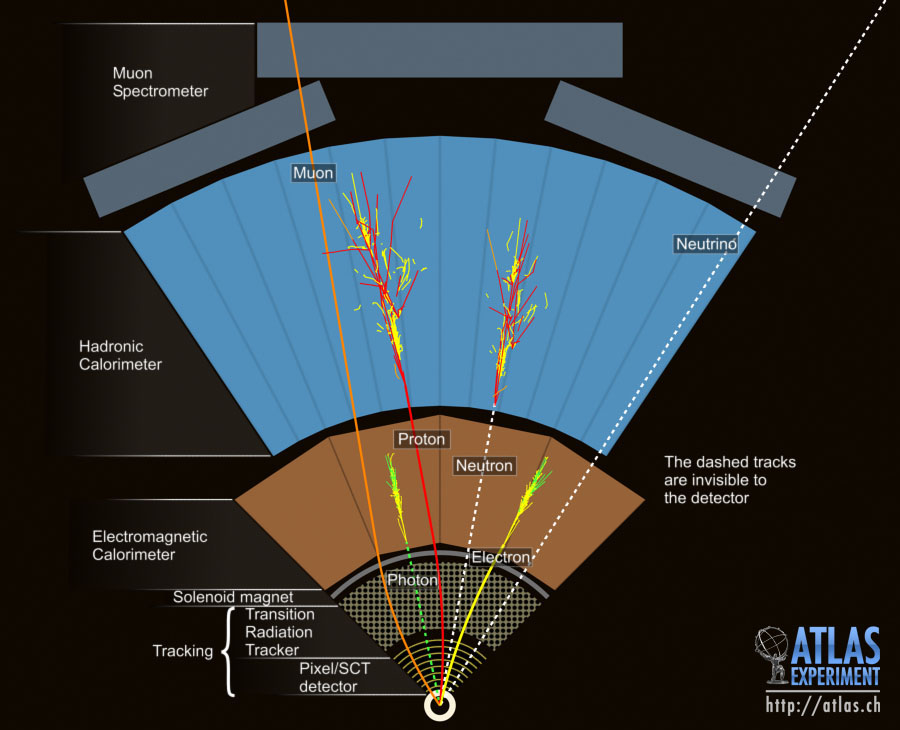
\includegraphics[width=0.75\textwidth]{Figures/Illustrations/detector.jpeg}
    }
    \caption[Event Cross Section in a computer generated image of the
    \acs{ATLAS} detector.]{Event Cross-Section in a computer generated image of the
    ATLAS detector \cite{PDetector}.}
    \label{fig:detector}
\end{figure}

\subsection{The Kinematics}
The kinematic variables of a particle collision are crucial in any \ac{HEP} analysis and are explained using simple 
geometry. In figure \ref{fig:Kinematics} I have drawn a simple axis to illustrate the kinematics of a particle in both the 
longitudinal (left) and transverse (right) plane. In a three-dimensional axis where the particles colliding travel along the 
z-axis, the zy-axis defines the longitudinal plane.  The angle between the z-axis and the direction of the momentum of
one of the particles, define the polar angle of said particle, $\theta$. The xy-axis define the transverse plane and the 
angle between the x-axis and the direction of the transverse momentum define the azimuthal angle, $\phi$.
\begin{figure}
    \centering
    \makebox[0.75\linewidth][c]{%
    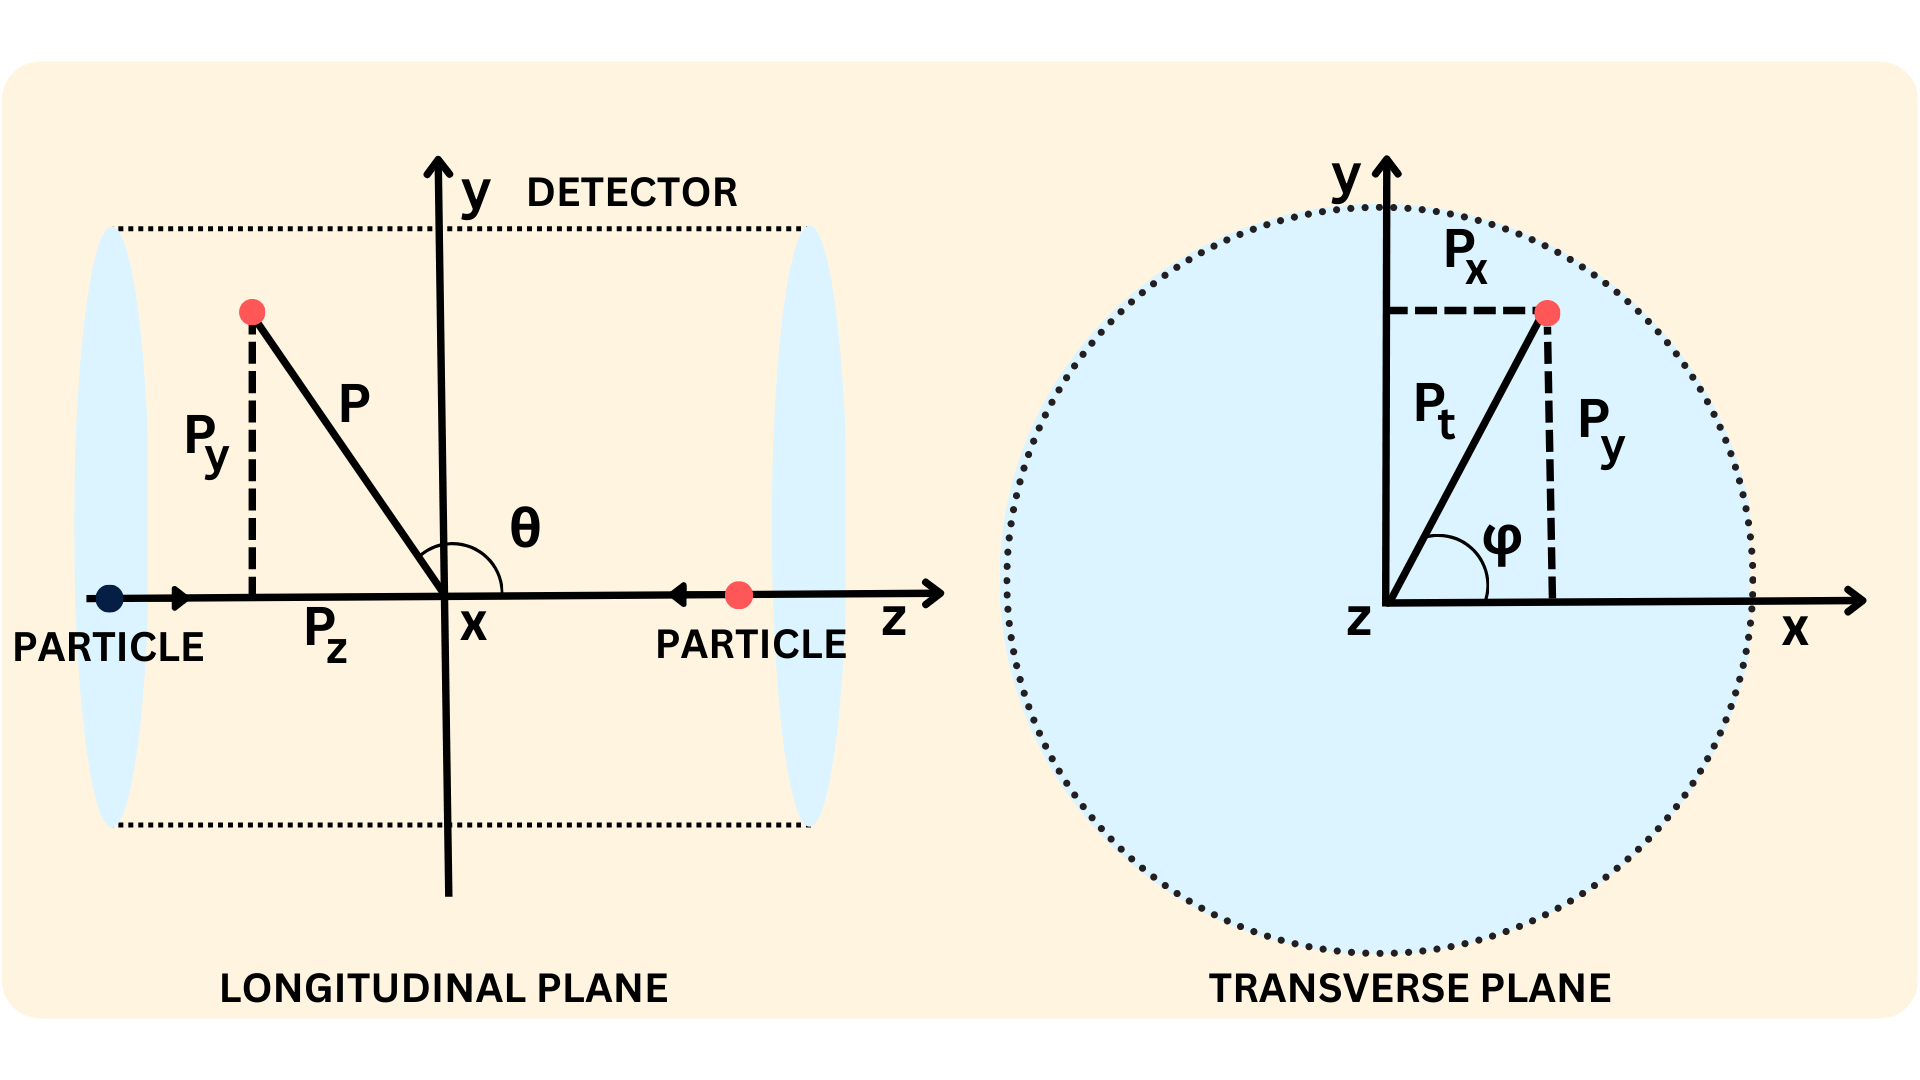
\includegraphics[width=0.65\textwidth]{Figures/Illustrations/Kinematics.png}
    }
    \caption[An illustration of the general kinematics in a particle-collision.]{An illustration of the general kinematics in a particle-collision, inspired by the 
    figure in the paper by Gramstad \cite{gramstad_searches_nodate}. The illustration shows both the 
    longitudial and transverse plane. }
    \label{fig:Kinematics}
\end{figure}
The transverse momentum and the azimuthal angel are both used in this analysis and are used to create further features. 
Instead of the polar angle, a preferred feature is the pseudorapidity, $\eta$. The pseudorapidity is defined as 
\begin{align}\label{eq:eta}
    \eta = -ln\left[tan\left(\frac{\theta}{2}\right)\right]
\end{align}
The pseudorapidity is a preferred feature to the polar angle because differences in $\eta$ are Lorentz invariant under boosts 
along the longitudinal axis. A large range of features are created using the variables described above. In the appendix I have 
added a summary of all the features used in this analysis (see table \ref{table:Features}). One of said features is the distance 
between the particle in the $\eta\phi-axis$, $\Delta R$. We define $\Delta R$ as 
\begin{align}
    \Delta R = \sqrt{(\Delta \eta)^2 + (\Delta \phi)^2}.
\end{align}

\section{The background channels}
The dominant SM backgrounds can be divided into two categories: (i) from leptonic $\tau$ decays and (ii) from fake leptons. In the first category, the dominant process is the pair production of $W Z$ with $W$ decaying leptonically and $Z \rightarrow \tau \tau$. The trilepton final states with no-OSSF pairs can arise from the subsequent leptonic decay of $\tau$ 's. We estimate this background process via Monte Carlo simulations.
\\
The dominant processes of the second category are $\gamma^{*} / Z+$ jets and $t \bar{t}$, where two leptons come from $\gamma^{*} / Z \rightarrow \tau \tau$ or the prompt decay of $t$ and $\bar{t}$, and a third lepton is faked from jets containing heavy-flavor mesons.
\begin{figure}
    \makebox[0.75\linewidth][c]{%
    \centering
    \begin{subfigure}{.2\textwidth}
        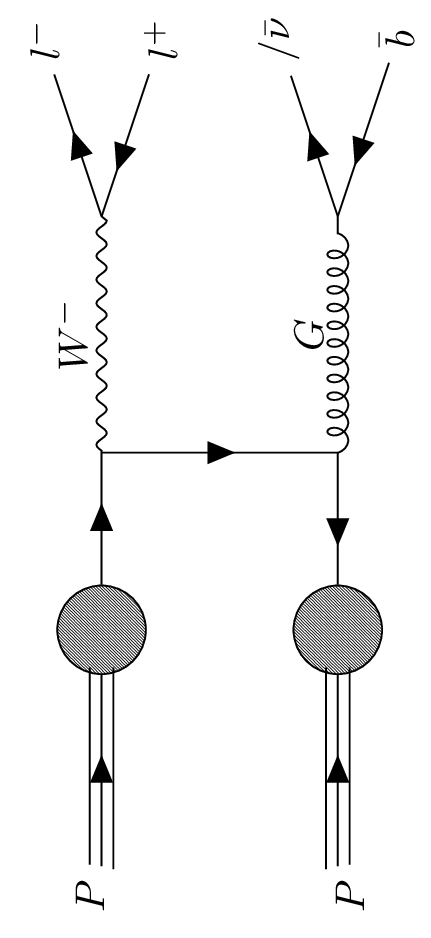
\includegraphics[width=\textwidth, angle = -90]{Figures/w_pjets.png}
        \caption{}
        \label{fig:w_pjets}
    \end{subfigure}
    \hfill
    \begin{subfigure}{.2\textwidth}
        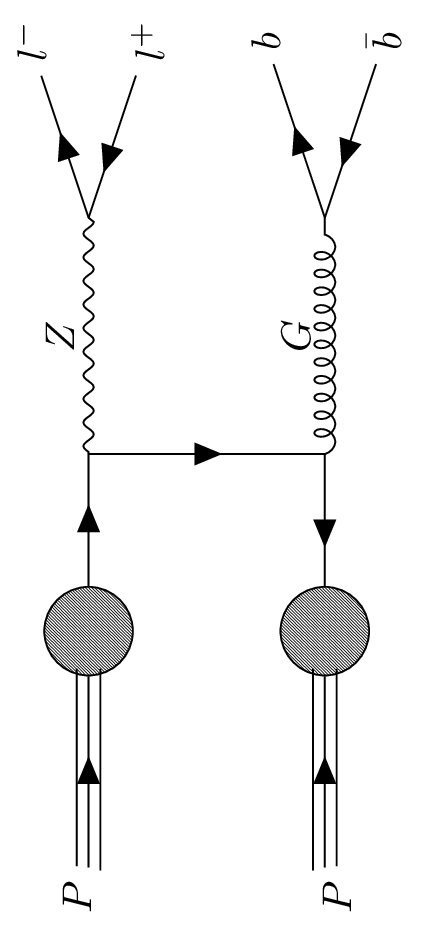
\includegraphics[width=\textwidth, angle = -90]{Figures/Z_pjets.png}
        \caption{}
        \label{fig:z_pjets}
    \end{subfigure}
    }
    \caption{}
\end{figure}
\section{The Signal}\label{sec:signal}
% \subsection{Heavy Neutral Lepton}
% \begin{figure}
%     \centering
%     \makebox[0.75\linewidth][c]{%
%     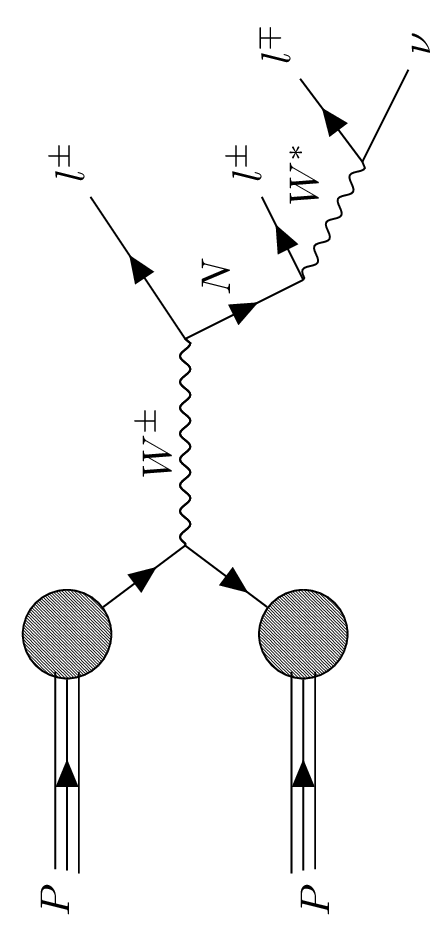
\includegraphics[width=0.225\textwidth, angle = -90]{Figures/FDiagrams/HNLSignal.png}
%     }
%     \caption{The Feynman diagram of the signal-channel.}
%     \label{fig:signal}
% \end{figure}
% \subsection{Neutralinos}
In this thesis, I will compare \ac{ML} models in their ability to learn the trends of the data which will contribute  
in our ability separate the signal from the background. Specifically for this thesis, I will be studying an expansion of the 
\ac{SM} which includes super symmetry (see section \ref{subsec:SS}). The signal I will aim to separate from the background, is one 
which produces a WZ pair, through two neutralinos. In figure \ref{fig:signal}, I have drawn a Feynman diagram for such a process.
The Feynman diagram shows a pair of neutralinos, the two lightest neutralinos introduced by the \ac{MSSM} ($\tilde{\chi}_1$ and $\tilde{\chi}_2$), 
and where each neutralino produces a boson (W and Z respectively) and a $\tilde{\chi}_1$. Given that the neutralinos in the final state 
are neutral, there are three leptons and a large amount of missing energy in the final state.
\begin{figure}
    \centering
    \makebox[0.75\linewidth][c]{%
    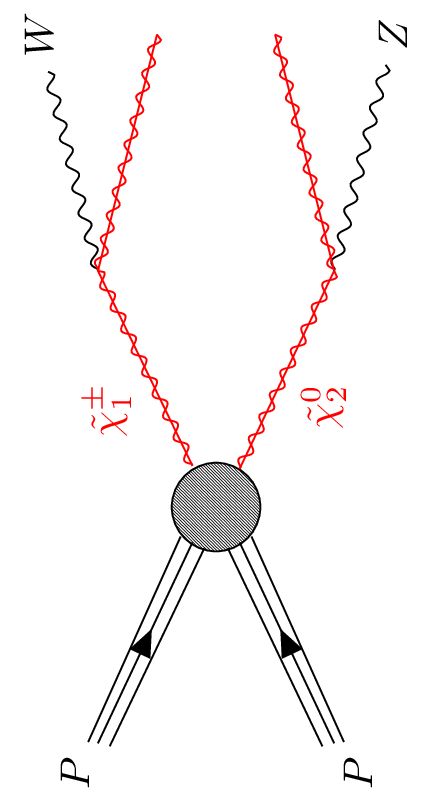
\includegraphics[width=0.225\textwidth, angle = -90]{Figures/FDiagrams/WZSignal.png}
    }
    \caption{The Feynman diagram of the signal-channel.}
    \label{fig:signal}
\end{figure}



%%%%%%%%%%%% ML %%%%%%%%%%%%%%%%%%%%%%%%%
\chapter{Introduction to supervised and unsuperised machine learning}\label{chap:Intro ML}
Machine learning is rapidly becomming an overwhelming presens in many different scientific fields.
In areas ranging from cancer research to stock-trading, machine learning is being applied to probelms
once thought as impossible to solve. Particle physics, like many other fields is no exeption. Jet flavor classification \cite{Guest_2016}, 
separating jets from gluons \cite{PhysRevD.44.2025} or using \ac{ML} to create efficent \ac{SR} are just some examples
where \ac{ML} is a vital tool. The traditional approach for ML in high-energy physics is through the use 
of supperivsed learning. \ac{DNN}


\section{Machine Learning}
\section{Phenomenology}\label{sec:MLPhen}
\ac{ML} models differs from other analysis tools in their ability to
learn. Where a purely analytical model is static in both method 
and performance, a \ac{ML} model aims to be dynamic and self 
improving. \ac{ML} utilizes data to leverage towards an optimal
model. The extent of utilization of data defines a \ac{ML} model as being
either \emph{supervised}, \emph{semi-supervised} or \emph{unsupervised}. In the case 
of supervised \ac{ML}, a set of \emph{targets} are provided along with the
data which allows a \ac{ML} model to learn how to map a set of inputs to a target. In this 
thesis I will use the notation of $X = [\bf{x}_0,\bf{x}_1,\bf{x}_2,...,\bf{x}_N]$ to refer to 
a data set, $T = [t_0,t_1,t_2,...,t_N]$ to the corresponding target and $Y=[y_0,y_1,y_2,...,y_N]$ 
to the output of the model where N is a number of points. The data sets contain a set of vectors with length equal to the number 
of features. The target and output could similarly contain vectors, but will in this thesis be restricted 
to scalar values. Generally, the target values can be both continues values, in which case the \ac{ML} 
method aims to perform a \emph{regression}, or discrete values, in which case the \ac{ML} method aims 
to perform a \emph{classification}. 
\\
The goal of supervised learning is that the model can apply any attained knowledge from 
the study of a set of inputs and targets to predict the target of a new dataset. 
The success of any prediction is dependent on the quality of the 
data used during training, or \emph{training-data}. The training-data is required to 
be both representative of any trends you hope to detect in the new data set (test-data)
and be of sufficient amount. The latter point stems from a phenomenon known as \emph{over-fitting},
which is a problem where the training data becomes overly specialized to only predict 
the target of the training-data, and nothing else\footnote{More on this in later sections.}.
In this thesis the main focus will be on the application of supervised learning.
\\
In the case of unsupervised \ac{ML}, no target is provided. The motivation for unsupervised
learning is to create a model which is independent of any target. Such models are often 
useful in the case where one is not certain what one is looking for. An independence of target
means that the model is not overly sensitive to any specific trends or patterns, we call
this being \emph{unbiased}. Instead of learning to detect or predict specific phenomenon,
unsupervised learning is often used to detect anomalies in the data, which means it relies
heavily on statistics. Because of this, some use the term \emph{anomaly detection} and 
unsupervised learning interchangeably.
\\
Semi-unsupervised learning is a loose term
which finds itself in the middle of the previous two. It often refers to methods where 
no concrete target is provided, but instead uses the data provided to create a target. The goal 
is to alleviate as much bias as possible, but at the same time converge towards the usually 
superior performance of supervised learning.  
\section{Optimization}\label{sec:Opti}
For a general function $g$ dependent one a set of parameters $\boldsymbol \theta = 
\{\theta_0,\theta_1,...,\theta_{N_\theta}\}$, the goal of optimization is to find 
optimal parameters as defined by a predicated goal. In our case we are interested in 
finding the set of parameters corresponding to the minimum value of $g$. Several methods
can be applied to optimization problems, all with their own advantages and disadvantages.
In most methods the use of the gradient of the function, $\grad_\theta (g)$ is involved in 
one way or another. Many of the methods used in this analysis are based on one of the simplest 
optimization methods, the \emph{gradient descent}-method.
\subsection{Gradient Descent}
The gradient descent method aims to obtain the optimal parameters $\tilde{\boldsymbol\theta}$ 
through the application of the derivative of $g$ with respect to $\boldsymbol \theta$. When 
evaluated in a given point in the parameter space $g(\boldsymbol \theta_i)$ the negative of 
the gradient $\grad_\theta (g)$, is used to move $\boldsymbol \theta_i$ closer to $\tilde{\boldsymbol\theta}$.
The negative is used due that $-\grad_\theta (g)$ corresponds to the direction for which a 
small change $d\boldsymbol\theta$ in the parameter space will result in the biggest 
decrease in the cost function. Finding the minimum value is an iterative process, meaning
the steps in the direction of $-\grad_\theta (g)$ is finite. The size of the step is a
hyperparameters decided by the user and is called the learning rate, $\eta$. The evolution 
from a step i to $i+1$ becomes
\begin{align}
    \boldsymbol{\theta}_{i+1}=\boldsymbol{\theta}_i-\eta \cdot \nabla_\theta g\left(\boldsymbol{\theta}_i\right).
\end{align}
Choosing the learning rate can drastically effect the performance of the gradient descent method. 
Too large and one risks "jumping" over the true minimum or simply never allowing for parameters
to reach a high accuracy. Too small and one risks having to spend computation time beyond reason. 
\subsection{Adam}


\section{Hyperparameters}
The tuning of parameters is a vital part of building an optimal \ac{ML}
model, though not all parameters are set during training. Parameters 
that are chosen prior to training are called \emph{hyperparameters}. We differentiate
between two types of hyperparameters; model hyperparameters and algorithm 
hyperparameters. Model hyperparameters refer to parameters used to define the 
architecture of the model. Examples of this could be the size and deepness of 
a \ac{NN} or the maximum deepness of a \ac{DT}. These parameters are not tuned
during training, but will nonetheless have a great impact on the performance 
of the model. Algorithm hyperparameters on the other hand, do not have a direct impact 
on the performance of the model. These are parameters that mainly effect the 
effectiveness and quality of the training process. Examples of this are the 
learning rate of a \ac{NN}, or the batch-size used during training. Regardless 
of if we are discussing model- or algorithm hyperparameters, it is in our interest
to find the optimal choice of parameters. The choice of parameters is made 
prior to the final training, and will be discussed in the following section.
\section{Data Handling}\label{subsec:Scaling}
As previously mentioned, the data used in \ac{ML} is as, if not more, important than the model itself. 
As a consequence, there are several steps taken to ensure that the data is in a good state before 
we apply the \ac{ML} models to it. In this section I will discuss some of these aforementioned steps, both 
what they do and what each step hopes to achive.
\subsection{Feature Scaling}
The range of values for the different data features can vary immensely, and for most 
cost functions, this is a problem. For some features, a deviation on the magnitude 
of $10^3$ can be a good approximation, whereas for others it can be a vast 
overestimation. When a model is to define which direction it wants to tune, it is 
crucial that the errors across all features are weighted equally. Scaling aims to alleviate 
this issue by transforming all features to have a relatively equal range of values while
simultaneously preserving all information regarding each feature. Exactly how one chooses 
to scale the data heavily affects the performance of the model and is regarded as a hyperparameter 
of the model. 
\subsubsection{Standard Scaler}\label{subsubsec:StandardScalar}
In this analysis, I decided to use the highly popular scaling method, the \emph{standard scaler}. 
The standard scaler implemented in this study uses Scikit-learns's \texttt{StandardScaler}
\cite{StandardScaler}. The standard scaler function scales each feature individually by subtracting 
the mean and dividing by the standard deviation. In doing so the resulting scaled data has a mean 
of 0 and a standard deviation of 1. Mathematically the standard scaler, $\mathcal{S}$, transforms 
a data set, $X$, as 
\begin{align}
    \mathcal{S} \left(X\right) = \frac{X - \boldsymbol{\mu} _x}{\boldsymbol{\sigma}_x} ,
\end{align}
where $\boldsymbol{\mu} _x$ and $\boldsymbol{\sigma}_x$ are vectors with the elements being 
the mean and standard deviation for each feature, respectively.
\subsection{Principal Component Analysis}\label{subsec:PCA}
\acf{PCA} is a dimensionality reduction technique used in many analyses. The goal of
\ac{PCA} is to reduce the dimensions of a high-dimensional data set while at the same time conserving as 
much of the variance (or value spread) in the data as possible. The motivation behind dimensionality reduction 
is (mainly) rooted in two points. The first is noise reduction. Some features could not only be non-contributing 
during training, but could even introduce noise. The second reason is lack of convergence. In a large 
data set with many features and different classifications (in our case channels), a \ac{ML} could struggle
to identify the most important patterns. By reducing the dimensionality in the data, the hope is that this 
would be easier. 
\\
In short, a \ac{PCA} finds the direction in the feature space along which the data has the largest 
variance (called principal components), using a linear combination of the original features, and projects the
data upon it, creating a new data set. The principal components are ordered such that the first captures the most variation,
the second captures the most variation orthogonal to the first and so on. Before applying the \ac{PCA}, it is essential to 
scale the data, to ensure a realistic representation of the variance in each feature.  We can summarize the algorithm of the 
\ac{PCA} in the following 6 steps:
\begin{enumerate}
    \item Center the data around 0 by subtracting the mean from each feature.
    \item Calculate the covariance matrix to find the covariance 
                             of each feature pair.
    \item Calculate the eigenvalue and eigenvectors of the covariance matrix.
    \item Order the eigenvector by size of the eigenvalues to define the directions 
                             in the feature space with the largest variance.
    \item Cast the data along these directions to form a new data set with 
                             the new features ranked from largest to lowest variance.
    \item Remove the features with the least variance according to some threshold
                            defined by the user.                      
\end{enumerate}
The threshold mentioned in the final point, is decided by the user, and defines how much of the variance from the original data 
set should be included. For example if the threshold is set to $70\%$, $X$ number of the last features will be removed such 
that at least $70\%$ of the variance is preserved.
\\
In figures \ref{fig:PCA1} and \ref{fig:PCA2} I have plotted the distribution of 10, 100 and 300 samples 
for the features with the most and second most variance (\ref{fig:PCA1}), and least and second least 
variance (\ref{fig:PCA2}) after applying \ac{PCA} to our data set. In this \ac{PCA} I am yet to remove features, 
so all four features are taken from a data set where all the variance is still conserved. Each color in the figures 
represent different categorize of collisions, i.e. $t\bar{t}$ or diboson. With this in 
mind, the different scales on the y- and x-axis ($10^0$ for figure \ref{fig:PCA1} and $10^{-8}$ for figure 
\ref{fig:PCA2}) exhibit how the \ac{PCA} creates new features where there is a vast difference in variance 
(and therefore value to the analysis), and justifies how one can remove features while preserving most of the variance. 
In figure \ref{fig:PCA2} we observe that all channels exhibit the same distributions and are practically identical. 
In other words, these features would not contribute in training a model to distinguish the different channels. 
In comparison, figure \ref{fig:PCA1} displays large variance and individual patterns among the different processes.
\begin{figure}
    \centering
    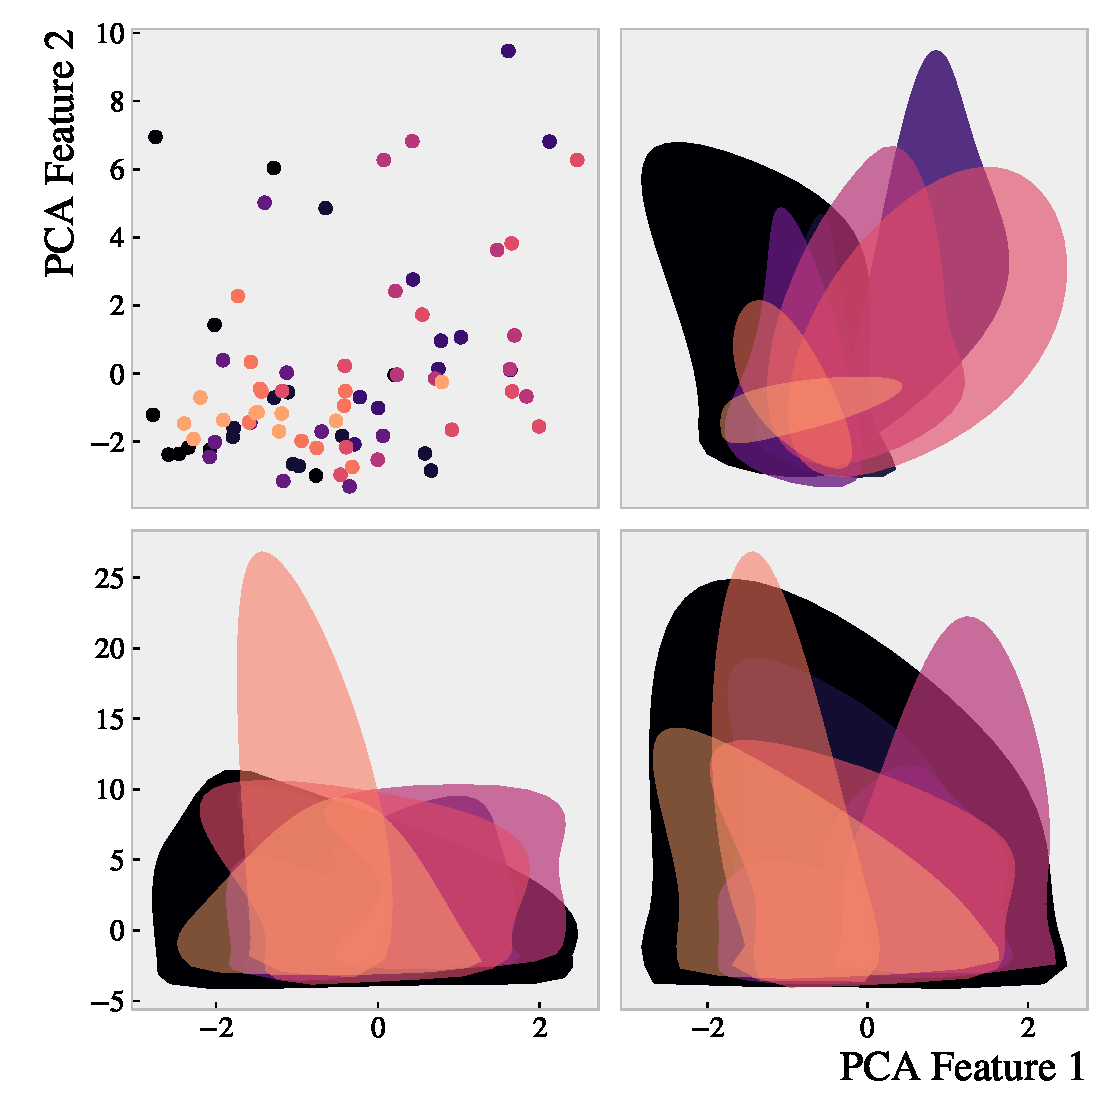
\includegraphics[width=0.6\textwidth]{Figures/MLResults/DataHandling/PCA/PCAPlotFirst.pdf}
    \caption[The value distribution of the two leading \acs{PCA}-features.]{The value distribution of 
    the two \ac{PCA}-features containing most variation for (left to right, up to down) 10, 10, 100 and 
    300 samples from each channel (visualized with different colors). Each sample filling the requirement with being less than one standard 
    deviation from the mean of both features, respectively.}
    \label{fig:PCA1}
\end{figure}
\begin{figure}
    \centering
    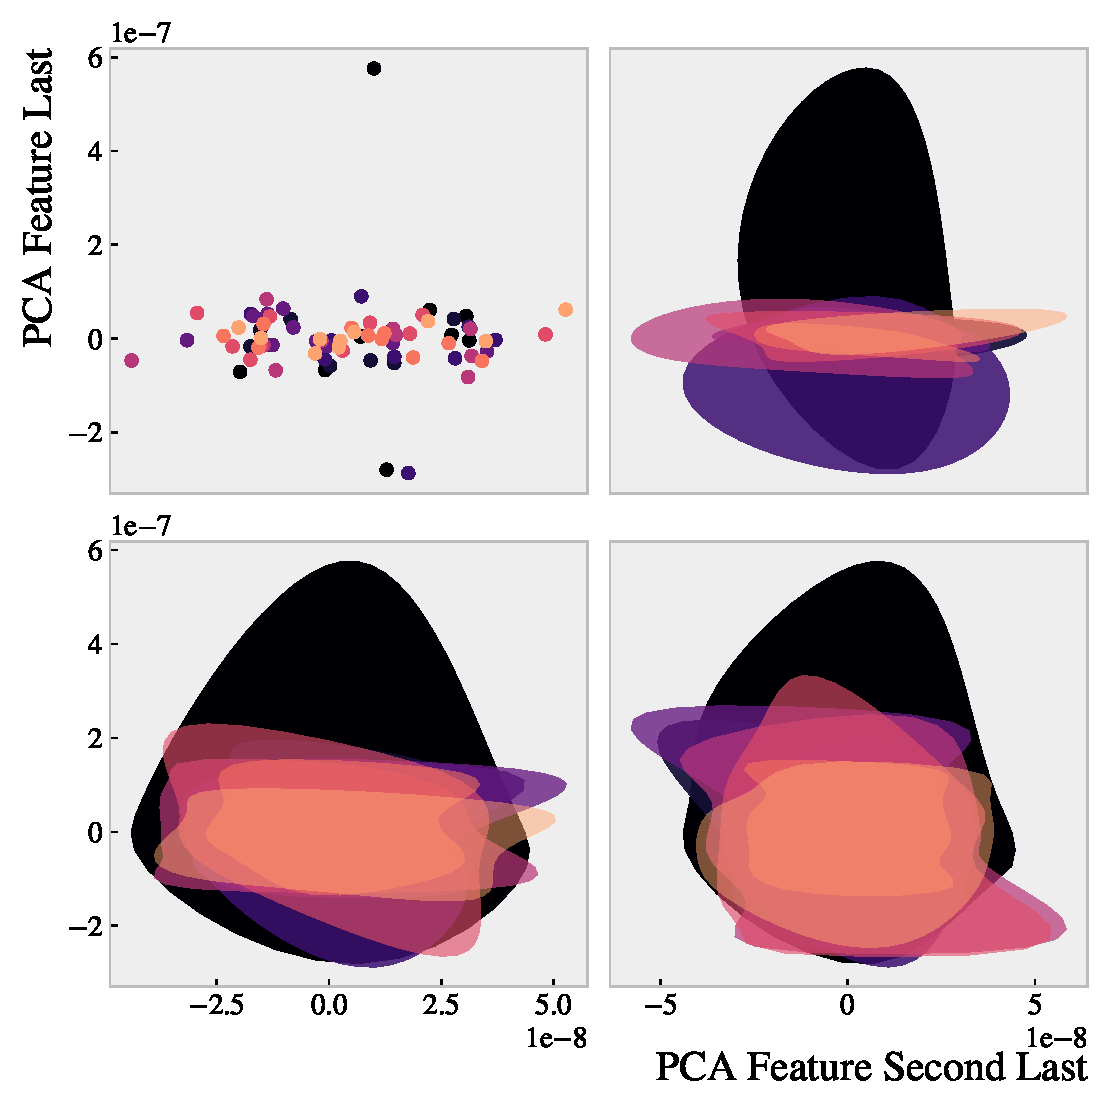
\includegraphics[width=0.6\textwidth]{Figures/MLResults/DataHandling/PCA/PCAPlotLast.pdf}
    \caption[The value distribution of the two last \acs{PCA}-features.]{The distribution of the two 
    \ac{PCA}-features containing the least amount of variation for (left to right, up to down) 10, 
    10, 100 and 300 samples from each channel (visualized with different colors). Each sample filling the 
    requirement with being less than one standard deviation from the mean of both features, respectively.}
    \label{fig:PCA2}
\end{figure}



\section{Regularization}
In \ac{ML}, overfitting occurs when a model becomes overly tuned to the training data and as a consequence 
fails to extract trends which would allow it to predict previously unseen data. The architecture of a \ac{NN}, 
the maximum depth of a boosted-\ac{DT} or even the size of the dataset can all contribute to overfitting. In the 
case of deep learning especially, overfitting can be a large problem and is therefore of focus in this thesis. Apart 
from predicting on a new data set, there are no rigid methods to detect overfitting. Instead, there exists many 
attempts to minimize the risk of it, we call these methods' \emph{regularization}. In \ac{ML}, regularization 
is known as any attempt to reduce the error in a prediction by reducing overfitting. Generally one can categorize
regularization as being either implicit or explicit. Explicit regularization means adding terms to the optimization 
problem. This is a very direct way of insuring no part of the model becomes overly dominant. Examples of this 
could be adding a penalty in the cost function of a \ac{NN} to ensure no weights become to large. Implicit
regularization is a less direct attempt of hindering overfitting. This could be changing the depth of the \ac{ML}-model,
varying the cost function or altering the data itself.
\subsection{Early stopping}
A simple implicit regularization method is to introduce \emph{early stopping} in the training pipeline. Early stopping 
simply means to stop training before the parameters of the model are allowed to over tune. The usual approach 
is to introduce a goal for the training, which when reached, ends the training. Examples of these goals could be a 
predetermined loss value on the training set or training until lack of progress on a second unseen dataset. The latter
approach is the one I will use in this thesis. 
\subsection{Ensembles}
When comparing different \ac{ML} methods by performance, more often then not the top performing model includes 
ensembling in one way or another. Like the word suggests, ensembling in \ac{ML} means using a collection of 
\ac{ML} models to create one complex model. There are many ways to create ensembles of models, most methods 
fall in to one of three categories; \emph{bagging}, \emph{boosting} and \emph{stacking}. Creating an ensemble of models 
through bagging, means to use several models each trained on their own sample from the same dataset. The overarching 
new model is created by averaging the predictions from the ensemble of models. The method seeks to create a unique set of 
models through exposing each individual model to different training sets. Boosting is different to bagging in that it uses 
the same training data on all the models. The diversity in the models when boosting, stems from intentionally choosing the 
architecture of the models such that it reduces the error made by the previous ensemble of models. Finally, stacking uses 
a predetermined model to decide how to combine the predictions made by the ensemble. More on the specifics of bagging, 
boosting and stacking in later sections.  

  

\section{Neural Networks}\label{sec:NN}
The concept of a \ac{NN} has been around for more than 80 years, and today they are one 
of the most popular and successful \ac{ML} methods. The key to its popularity stems from
its versatility, achieving high performance in a large range of both regression 
and classification problems. One of the defining qualities in a \ac{NN} is the 
possibility of diverse architecture, meaning that there are many
categories of \ac{NN}, where each category has an even deeper selection of
networks. Categories ranging from \ac{CNN}, \ac{RNN} to simple \ac{FFNN}, where each
category is specified for their own set of problems. In this section I will introduce 
some fundamental definitions in regard to \ac{NN}, and go through the underlying 
algorithm of the back- and forward propagation.

\subsection{General Structure}
There are often drawn comparisons between the structure of the neural network, 
and the way the human mind operates, hence neural. Similarly to the human mind, a \ac{NN} is 
composed of different neurons, or nodes communicating information backwards and forwards in different 
regions. In the case of a neural network we call these regions layers. All layers
are composed of a specified number of nodes. A \ac{NN} has three types of layers;
\emph{input layer}, \emph{hidden layer} and \emph{output layer}. There is only one input layer, and it has
the same number of nodes equal to the number of features for each data point. 
There can be an arbitrary number of hidden layers, with each hidden layer containing
an arbitrary number of nodes. Finally, the \ac{NN} has an output layer. The output layer
contains a number of nodes equal to the dimensions of the target.
\\
A \ac{NN} functions by passing information in between the different layers through 
nodes. The nodes are simply pockets of information, each containing a value. 
All the nodes in the input layer are (in most cases) connected to all nodes in the nearest hidden layer,
and likewise said hidden layer is connected to the next hidden layer. This structure continues
until we reach the final layer, the output layer. The structure is illustrated in figure
\ref{fig:NN}. The figure shows a simple \ac{NN} with a two-dimensional data set (two nodes in input layer),
two hidden layers with three nodes each and a one-dimensional target value. It also illustrates 
how a \ac{NN} aims to map from data to a prediction.
\begin{figure}
    \centering
    \vspace*{-12.5mm} 
    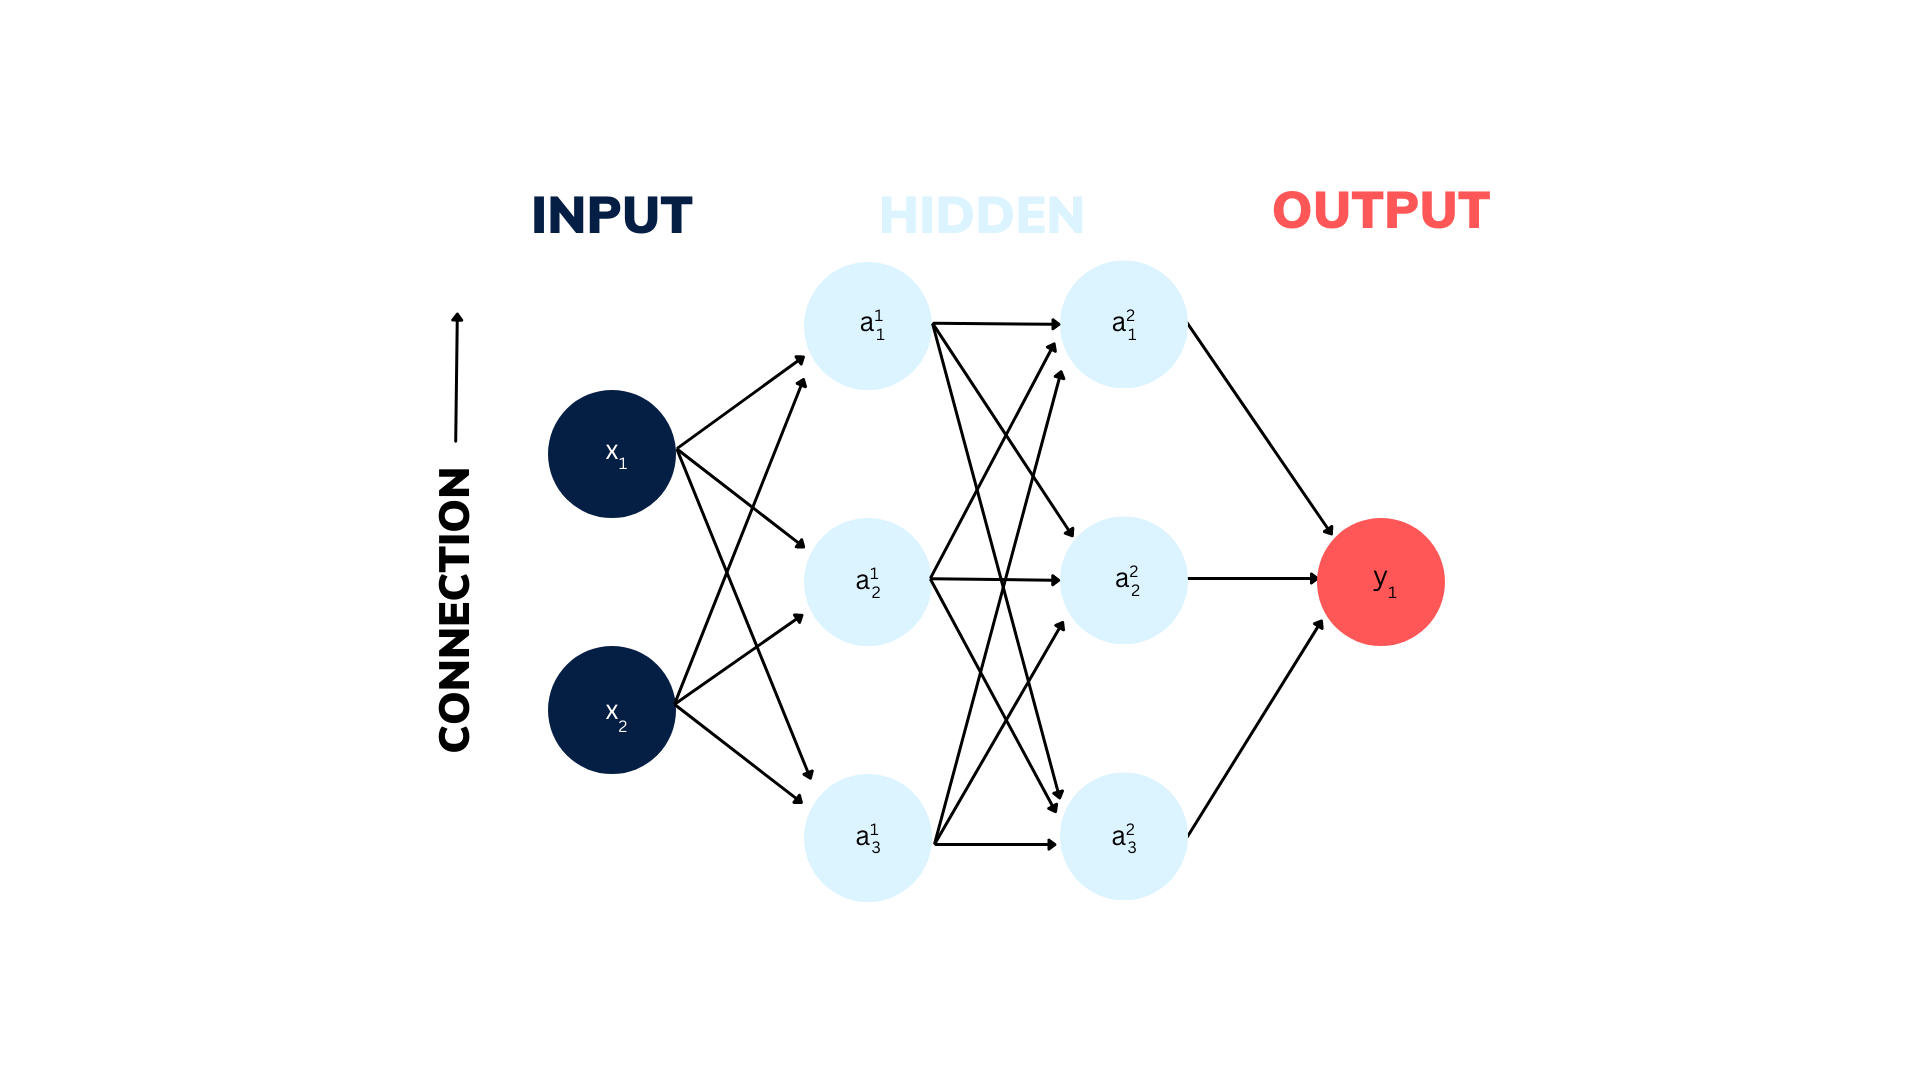
\includegraphics[width=0.9\textwidth]{Figures/Illustrations/Input_labels.png}
    \vspace*{-12.5mm} 
    \caption{An illustration of the architecture of a \acs{NN} with two hidden layers.}
    \label{fig:NN}
\end{figure}
In figure \ref{fig:NN} we can see how all the different nodes are connected, illustrated by 
the arrows. The passing of values between different nodes are controlled by a set of weights and
bias parameters. These parameters are defined for each connection and are what will be tuned 
during training. The weights and biases for a given connection of two nodes, defines the effect one node 
has on the other.
\\
In a traditional \ac{FFNN} the information is passed linearly (in figure \ref{fig:NN}, from left to right) 
in a process we call \emph{forward propagation}. Other variants can include the information taking a more 
complex route. It is often the route from input- to output layer that categorizes the type of \ac{NN}. In 
this report I used a set of simple \ac{FFNN}'s. 

\subsection{Feeding Forward}\label{subsec:FP}
With the structure described in the previous section, a trained model, $\mathcal{F}$, produces a prediction,
$Y$, for a data set, $X$, by passing information from input layer, through all hidden layers, to the output layer, 
which we call forward-propagation. In this section I aim to explain the underlying algorithm and math used by the 
\ac{NN} to map input to output. 
\\
We imagine the passing from hidden layer $l-1$ to $l$, where $l \in \{2,...,L \}$\footnote{There is a special
case for when $l=1$ which will be addressed in the next paragraphs.} and $L$ is equal to the
number of hidden layers. The activated value of a node in layer $l$, is defined as $a^l_j$ (as indicated by figure \ref{fig:NN}), 
where $j\in \{0,1,...,N_l\}$ and $N_l$ is equal to the number of nodes in $l$. The value of $a_j^l$ is defined as 
the \emph{activated} sum of all nodes in the previous layer, $a_j^{l-1}$ where the sum is weighted by a parameter $\bf{w} \sf _j^l$ 
and shifted by the bias, $b^l_j$ for $j\in \{0,1,..., N_{l-1} \}$. The activated value of a node j in layer l is defined as 
\begin{align}\label{eq:activated}
    z_j^l = \sum_{k=1} ^ {N_{l-1}} w_{kj}^la_k^{l-1} + b^l_j,
\end{align}
where $w_{kj}^l$ corresponds to the weight in $\bf{w} \sf _k^l$ specific for the connection between node k and j.
\\
To attain the full activated value, $a_j^l$ we pass $z_j^l$ through the \emph{activation function}. The activation function, $\sigma^l$ 
is a generally non-linear function used to control the limit or expand the value range for the node values. The activation 
function is general for all nodes in a given layer, but can vary in between layers. Therefore,
we find $a_j^l$ by the equation
\begin{align}\label{eq:ajl}
    a_j^l = \sigma \left (\sum_{k=1} ^ {N_{l-1}} w_{kj}^la_k^{l-1} + b^l_j\right ) = \sigma^l(z_j^l).
\end{align}
A more detailed illustration of the information passed from one layer to a node in the next layer is displayed 
in figure \ref{fig:WB}. In figure \ref{fig:WB}, we see all steps described in the process; \emph{(1)} all nodes in 
l-1 are summed with a corresponding weight, \emph{(2)} the sum is shifted by a constant term (bias), \emph{(3)} the 
scaled and weighted sum defines the inactivated value $z_j^l$, \emph{(4)} we define $a^l_j$ by passing the 
sum through $\sigma^l$.  
\begin{figure}
    \centering
    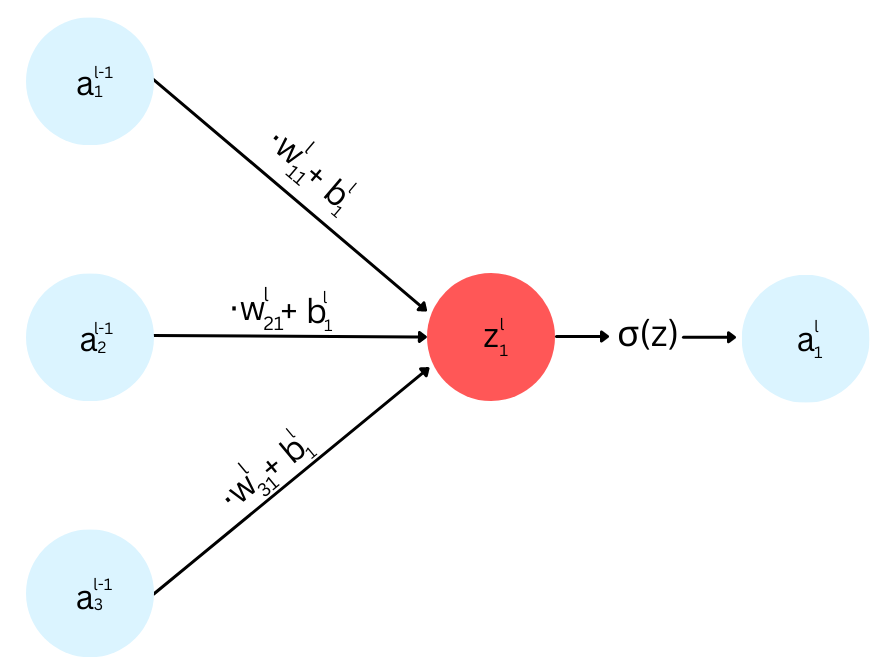
\includegraphics[width=0.5\textwidth]{Figures/Illustrations/WeightBias.png}
    \caption{An illustration of a forward propagation from one layer to a node in the next.}
    \label{fig:WB}
\end{figure}
This method is used to pass information between all layers, except between the first and the second. 
In this case we simply replace the activated term, $a_k^{l-1}$ in equation \ref{eq:ajl}, by the input data,
$x_i$ for $i\in\{0,1,...,N\}$, where N is equal to the number of features for the data. In the case $l=1$, \ref{eq:ajl} 
becomes
\begin{align}
    a_j^1 = \sigma \left (\sum_{k=1} ^ {N} w_{kj}^1x_k + b^1_j\right ) = \sigma(z_j^1).
\end{align}
And in the case where $l=L$, $a_j^L$ is equal to the final output. 
\subsection{Back Propagation}\label{subsec:BP}
The backward propagation acts as the engine that drives the training of a neural network. It has the purpose
of calculating the gradients of the \emph{cost function}, $\mathcal{C}$, with respect to the weights and biases of the network. 
The cost function defines to which metric we aim to optimize the network. When a neural network produces a prediction, $Y$, the error in the prediction
is defined by the cost function as $\mathcal{C}\left(Y, T\right)$, where T is the target. To minimize $\mathcal{C}$, the 
backward propagation utilizes the gradient with respect to the weights and biases in the network, as described in the section 
regarding optimization \ref{sec:Opti}. Instead of a direct calculation of the gradient, which is very computationally heavy, 
the backward propagation aims to calculate the gradient through a recursive algorithm which traces the error backwards through 
the network. It is this algorithm I will describe in this section.
\\
When minimizing the error defined by $\mathcal{C}$, we can apply several optimization algorithms described in 
section \ref{sec:Opti}. Common for the algorithms is the use of the gradient of the cost function with regard to 
the tunable parameters. In our case these parameters are the weights and biases, $w_{i,j}^l$ and $b^l_j$. The goal of 
the backward propagation is therefore to calculate the gradients $\partial \mathcal{C}/\partial w_{i,j}^l$ and
$\partial \mathcal{C}/\partial b^l_j$. 
\\
To begin with we can derive an expression for $\partial \mathcal{C}/\partial w_{i,j}^l$. We use the chain-rule to define 
\begin{align*}
    \frac{\partial \mathcal{C}}{\partial w_{i,j}^l} = \frac{\partial \mathcal{C}}{\partial z^l_j} \frac{\partial z^l_j}{\partial w_{i,j}^l},
\end{align*}
which we can simplify further by using equation \ref{eq:activated} to calculate the second term, which becomes
\begin{align*}
    \frac{\partial \mathcal{C}}{\partial w_{i,j}^l} = \frac{\partial \mathcal{C}}{\partial z^l_j} a^{l-1}_i.
\end{align*}
We can redefine the first term in the equation above as $\delta_j^l$ and write
\begin{align*}
    \delta_j^l \equiv \frac{\partial \mathcal{C}}{\partial z^l_j}
               = \sum_k \frac{\partial \mathcal{C}}{\partial z^{l+1}_k}\frac{\partial z_k^{l+1}}{\partial z^l_j}  
               = \sum_k \delta_k^{l+1}\frac{\partial z_k^{l+1}}{\partial z^l_j},
\end{align*}
where we have again used the chain rule for all contributing nodes. To calculate the final partial derivative we write
\begin{align*}
    \frac{\partial z_k^{l+1}}{\partial z^l_j} = \frac{\partial z_k^{l+1}}{\partial a^l_j}\frac{\partial a^l_j}{\partial z^l_j}
                                              = w_{jk}^{l+1}(\sigma^l(z_j^l))',
\end{align*}
where we have again used equation \ref{eq:activated}. This gives the expression for $\delta_j^l$
\begin{align}\label{eq:delta}
    \delta_j^l  = \sum_k \delta_k^{l+1}w_{jk}^{l+1}(\sigma^l(z_j^l))'  
\end{align}
Finally this gives us the expression
\begin{align}\label{eq:dw}
    \frac{\partial \mathcal{C}}{\partial w_{i,j}^l} = \delta_j^{l} a_j^{l-1}.
\end{align}
Next we want to derive $\partial \mathcal{C}/\partial b^l_k$. We simply use the chain rule and derive
\begin{align*}
    \frac{\partial \mathcal{C}}{\partial b^l_j} = \frac{\partial \mathcal{C}}{\partial z^l_j}\frac{\partial z_j^l}{\partial b^l_j},
\end{align*}
which from equations \ref{eq:delta} and \ref{eq:dw} is simply
\begin{align}\label{eq:db}
    \frac{\partial \mathcal{C}}{\partial b^l_j} = \delta_k^{l} \cdot 1 = \delta_j^{l},
\end{align}
From all three derived expressions, equations \ref{eq:delta}, \ref{eq:dw} and \ref{eq:db} we see that 
to calculate for all $l\in\{0,1,..,N_l\}$ we must first calculate $\delta_j^L$ and apply a recursive propagation.
To calculate $\delta_j^L = \partial \mathcal{C}/\partial z^L_j$ we again apply the chain rule with the assumption of the activated 
node in the cost-function, and we find
\begin{align}\label{eq:deltaL}
    \delta_j^L = \frac{\partial \mathcal{C}}{\partial a^L_j}\left(\sigma^L(z_j^L)\right)'.
\end{align}
This expression, similarly to equation \ref{eq:delta}, is dependent on the choice of $\mathcal{C}$ and 
the activation functions. Now that equation \ref{eq:deltaL} is defined, we can see that the
gradient of the parameters in all other layers can be calculated. A full \emph{epoch} is defined as 
a forward propagation which creates a prediction, followed by a backward propagation which tunes the parameters 
in an attempt to correct the errors in the prediction.
\subsection{Activation Functions}\label{subsec:activation}
As mentioned in previous sections, activation functions define how the weighted sum of the nodes in the previous layer 
define the value of the node in the current. There are many types of activation functions, 
where all have advantages and disadvantages. The choice of activation function for each layer is defined
before training, making it a hyperparameter. The activation functions applied and tested in this thesis are the following:
\begin{center}
\begin{itemize}
    \item  \emph{Sigmoid}\\  
    \begin{align*}
         \sigma{(z)} = \frac{1}{1+e^{-z}} = a \in [0,1]
    \end{align*}
    \item \emph{LeakyReLU}
    \begin{align*}
        \sigma{(z)} = \left(
        \begin{cases}
            z,& \text{if } z\geq 0\\
            \alpha z,              & \text{otherwise}
        \end{cases}\right)
        = a \in (-\infty, \infty),
   \end{align*}
   where $\alpha$ is scalar.
\end{itemize},
\end{center}
where $z$ is an inactivated node which is activated to define $a$, the activation.

\subsection{Network Ensembles, Dropout and LWTA Networks}\label{subsec:LWTA}
So far in the thesis, I have only covered dense layers, meaning that every node in a layer 
is connected to the nodes in the previous and following layer. 
This definition covers many, but not all hidden layers. Some layers do not pass values back and forth between 
nodes but instead dynamically change the architecture of the \ac{NN}. In this analysis, 
I have implemented both the \emph{dropout}-layer, and also a group of layers fitting the definition 
introduced in the paper \cite{srivastava_compete_2013}, as \ac{LWTA}.
\subsubsection*{Dropout}\label{subsubsec:Dropout}
The dropout layer functions by assigning a predetermined probability to each neuron in a given layer. Based on the 
probability, a number of neurons (dependent on the probability) is dropped in each forward pass. By doing this the 
dropout layer creates a different architecture for the network for every round of training. Each unique architecture represents 
its own network in what becomes an ensemble of networks. 
\\
As mentioned in previous sections, creating ensembles of models is a form of regularization. In the case of 
dropout, it minimizes the risk of overfitting by hindering a phenomenon known as complex co-adaptation. Complex
co-adaptation happens when a neuron becomes overly dominant such that neighboring neurons no longer contribute (relative
to the dominant neuron) and therefore lack the motivation to tune. When this happens, networks become fragile and overly 
specialized to the training data. By randomly dropping neurons, the neighboring neurons are no longer allowed to be passive 
and are forced to tune to compensate. During evaluation, the dropout layers no longer take action. Instead, the dropout rate 
(frequency of drop) $r$ is used to scale the weights by a factor $1-r$. The prediction made by the resulting 
model can therefore be seen as the average of all the smaller networks. In other words, a neural network containing dropout layers 
can be viewed as a bagging ensemble (see subsection \ref{subsec:Ensembles}). 

\subsubsection*{Channel-Out}\label{subsubsec:Channel-Out}
Dropout layers are not the only layers to dynamically change the architecture of a network. In this thesis I additionally 
explored the lesser known, \emph{Channel-Out}-layer as introduced in the paper by Wang et al. \cite{wang_maxout_2013}. 
Channel-out, similarly to dropout creates an ensemble of networks by removing a set 
of nodes for each round of training. Contrary to dropout, channel-out does not choose the nodes to drop at random,
but instead creates local \emph{units} by grouping the nodes, and removes all nodes except the node with the largest
activation in each respective unit. The 'removed nodes' are multiplied by 0, as to remove any contributions to the next layer.
The goal of channel-out is to create an ensemble of networks through \emph{pattern-specific paths},
where each network is specialized for a given pattern in the data. This would create an ensemble of networks, which not only applies a form of 
regularization, but also improves a phenomenon known as \emph{long-term memory} in the model. The phenomenon of long-term memory is discussed in 
the article by Srivastava et al. \cite{srivastava_compete_2013}, and is simply a measure of how well a model is able to retain information on a data set, A, after 
training on an additional training set, B. This effect is also relevant for the two layers I will discuss in the next sections.
\\
In this thesis I have implemented the layer such that upon prediction, the redimensionalization 
is still active. This means that for each data point, a neural network is chosen based on the specific activations in 
each of the nodes. In other words, the channel-out layer creates something resembling a stacking ensemble (see subsection 
\ref{subsec:Ensembles}). 
\subsubsection*{Stochastic-Channel-Out}\label{subsubsec:stochchannelout}
As I will describe in further detail in sections to come, I choose to implement the channel-out layer myself. A consequence of this 
was that I was able to experiment with it. In section \ref{subsubsec:Dropout}, I described the issue of complex co-adaptation. I also described 
a possible solution to the issue, the dropout layer. Although dropout and channel-out function rather similarly, they do not deal 
with this issue in the same way. Where the dropout layer will force dormant nodes to contribute in the training by allowing for dominant
nodes to be dropped, the channel-out would instead allow for dominant nodes to take further control inside their respective unit.
\\
To remedy the issue of complex co-adaptation inside the units, I proposed a new layer, the \acf{SCO}. \ac{SCO} functions similarly to channel-out, 
with the exception of the units. Where the channel-out layer utilizes static local units\footnote{I.e. the nodes are placed in local units in the beginning of 
training and held constant throughout.} throughout training, the \ac{SCO} instead utilizes dynamic units which change for each data point. In other words, 
for each data point, each node would potentially have a new group of nodes to compare with when finding the largest activation.
The goal of the \ac{SCO} is to capitalize on the randomness of the dropout layer and the pattern-specific paths' aspect from the 
channel-out layer.
\\  
In the same manner as for channel-out, the redimensionalization is active during prediction and training for the \ac{SCO}. This 
means that also the \ac{SCO} creates an ensemble resembling a bagging ensemble.
\subsubsection*{Maxout}\label{subsubsec:maxout} 
Additionally to the channel-out I will be applying a second layer discussed in the paper by Wang et al. \cite{wang_maxout_2013}, 
the \emph{Maxout} layer. The maxout layer functions very similar to the channel-out with a small difference in the dropping of nodes. 
In the dropout layer, nodes are dropped by neglecting all contributions from said node, or in other words by multiplying the activation 
from the dropped nodes by zero. This is replicated in both the channel-out layer and the \ac{SCO} layer. In doing so all nodes, activated 
and dropped alike, possesses their own set of weights and biases. This is not the case for the maxout layer.
In the maxout layer, each unit possesses just one set of weights and biases. For each forward pass in the network, the largest activated 
node will contribute to the nodes in the following layer using the same weights and biases as the rest of the nodes in the units. However, 
the nodes only share parameters connected to the layer in front, not behind. This allows for the maxout layer to have fewer parameters to 
tune, while at the same time building pattern-specific pathways similar to channel-out and \ac{SCO}. \\
\begin{figure}
    \centering
    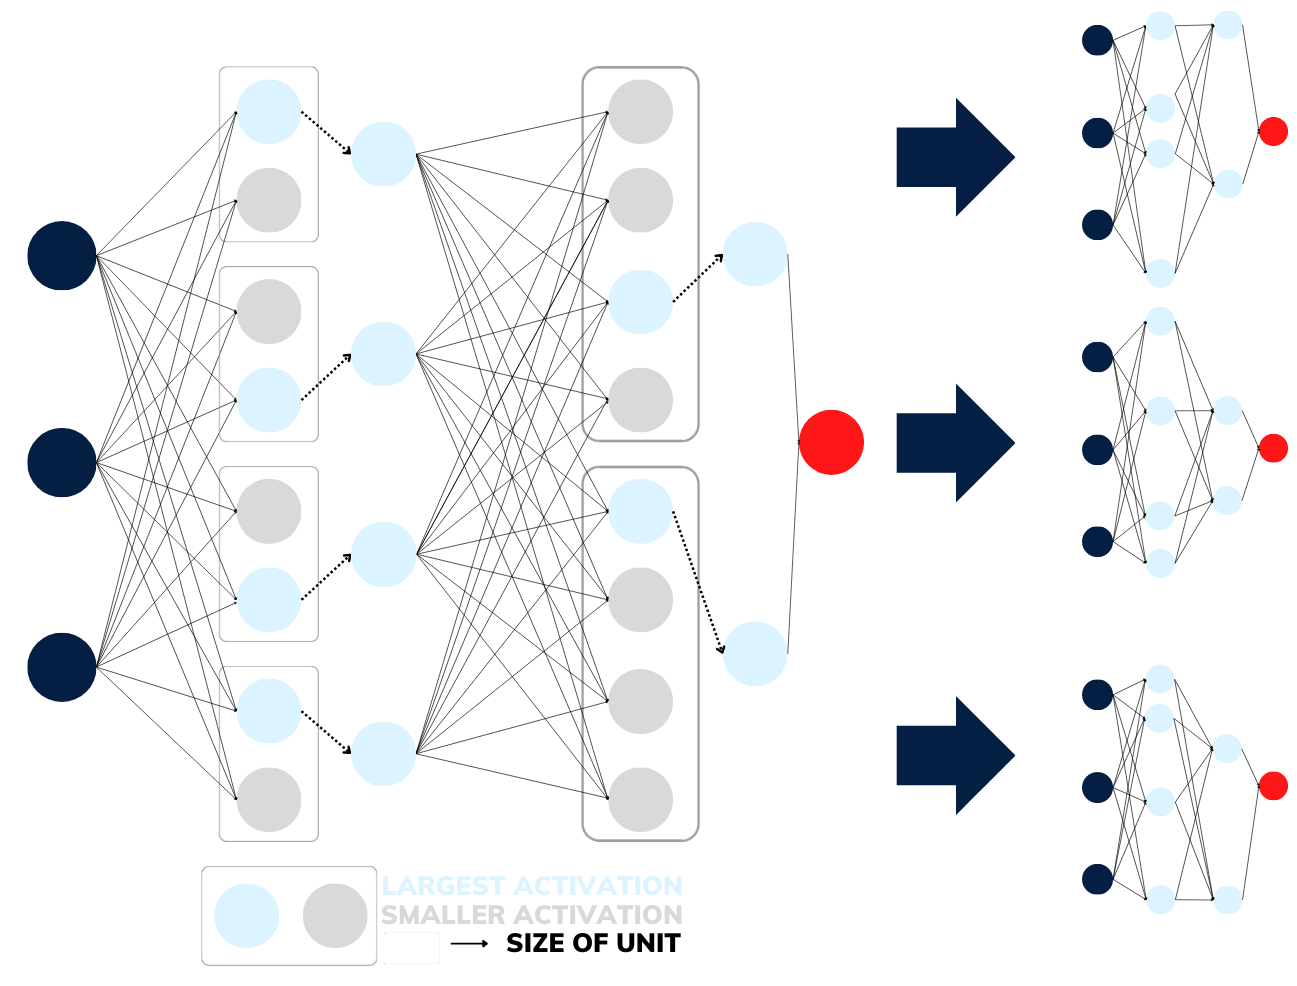
\includegraphics[width=0.7\textwidth]{Figures/Illustrations/Max_out.png}
    \caption[An illustration of a Neural network with two hidden layers using the maxout layer.]{An illustration of a Neural network 
    with two hidden layers, each with 8 neurons. The first and second hidden layers have a maxout activation layer with four and two 
    units respectively. The figure also illustrates the resulting ensemble of smaller neural networks as a consequence
    of the maxout activation layers. }
    \label{fig:Max_out}
\end{figure}
In figure \ref{fig:Max_out} I have illustrated a maxout network. The figure shows a \ac{NN} with two hidden layers
with eight nodes each. In the first hidden layer the maxout layer creates four units, each containing two nodes, and in the 
second layer the maxout creates two units with four nodes each. The resulting output from the first layer is the 
four nodes with the highest activation in their respected unit, likewise the second layer's output is two nodes.
To the right of the network in figure \ref{fig:Max_out}, I have illustrated how the different configuration of 
paths through the network creates an ensemble of networks with their own architecture. Note in the figure how, as described in the 
previous paragraph, each node possesses its own connections to the previous layer, while sharing the connections with the 
rest of the unit, to the next. In figure \ref{fig:NetEnsembleComp} I have drawn a separate illustration to show how 
this differs from both channel-out and \ac{SCO} in this regard. Figure \ref{fig:NetEnsembleComp} illustrates how 
all three layers redimensionalize the network, how channelout and \ac{SCO} differ from maxout in regard to the relationship 
between units and parameters and finally how channel-out differs from \ac{SCO} in choice of units\footnote{In figure 
\ref{fig:NetEnsembleComp} this is highlighted by the different colors surrounding the nodes in \ac{SCO}, where each color 
represents a unit.}
\begin{figure}
    \centering
    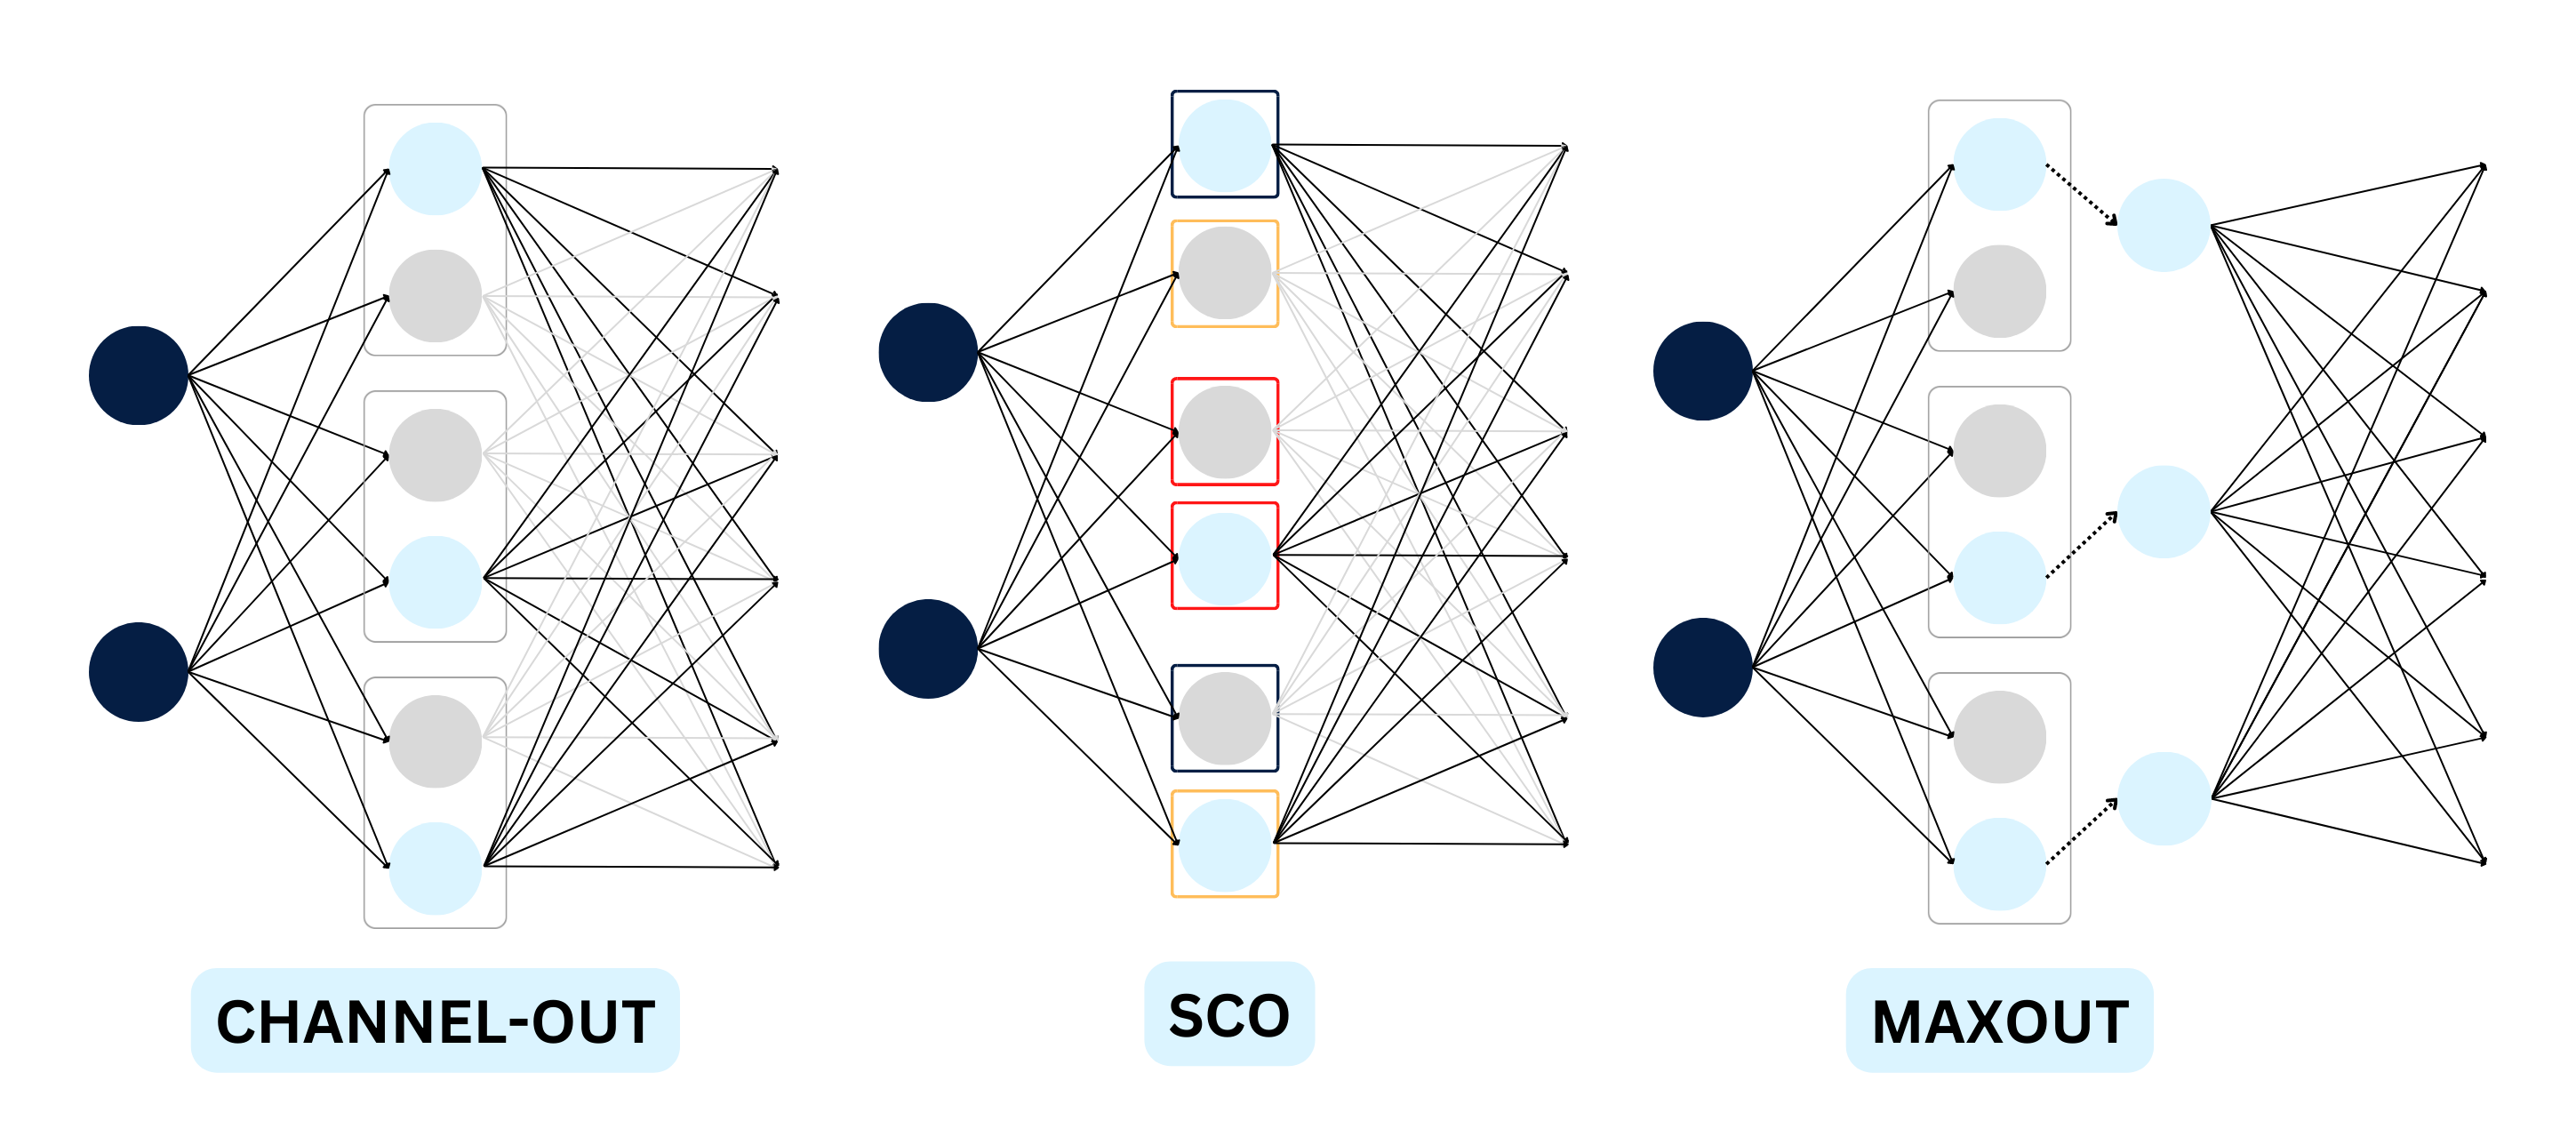
\includegraphics[width=0.8\textwidth]{Figures/Illustrations/EnsembleComp.png}
    \caption[An illustration of three different layers, channelout, \acs{SCO} and maxout.]{An illustration of three different layers, channelout, 
    \ac{SCO} and maxout. The figure shows how each layer redimensionalize the network and how channelout and \ac{SCO} differ from maxout in regard 
    to the relationship between units and parameters. The gray lines and nodes represent dropped nodes, whereas the blue nodes and dark lines represent
    the nodes which are allowed to contribute. In the case of \ac{SCO} the different colors surrounding the nodes represents different units, which 
    visualizes how any set of nodes could define a unit.}
    \label{fig:NetEnsembleComp}
\end{figure}
\subsection{Parametrized Neural Network}\label{subsec:PNN}
In this thesis I will be studying \ac{BSM}-simulations produced with a diversity in choice of free parameters. This
means that the signal is itself diverse. The free parameters studied in this thesis are the mass of 
new particles. The mass of a hypothetical particle in a given \ac{BSM} theory can greatly alter the feature space
spanned by processes including said particle. This means that a single \ac{ML}-model could potentially struggle to tune 
according to multiple signal samples that differ only in the mass of the hypothetical particle. The obvious solution to 
this problem is simply to implement one model per mass combination, or choice of mass, and simply reusing the background. 
Although this approach is very popular, I have decided not to use it for (mainly) three reasons:
\begin{itemize}
    \item This approach has been carefully studied for many years, and leaves little room to further exploration. 
    \item Some signals overlap in the feature space. This means that by neglecting signals with relative 
          similar mass, you could be neglecting statistics which could help tune to your original signal. 
    \item By including two signals with relatively similar masses in the training, some\footnote{See the paper by Baldi et al. \cite{PNN}.} 
          suggest that the model would be able to interpolate between the masses and cover a larger search area.
\end{itemize}
When the data set, $X$, is dependent on a set of free parameters, $\theta = [\theta_0,\theta_1,\theta_2,...,\theta_N]$,
we can write $X(\theta)$. For a single neural network trained on a set of parameters, we define the model as 
$\mathcal{F}(X(\theta))$. In the case where we build one model for each choice of parameter, we get a set of models
defined as $\{ \mathcal{F}_a(X(\theta_a))$, $\mathcal{F}_b(X(\theta_b))$, ...,$\mathcal{F}_c(X(\theta_c))\}$, where
a, b and c are indices which correspond to individual choices of parameters respectively. 
\\
In the paper by Baldi et al. \cite{PNN}, they propose a separate solution to the problem than the one proposed above, the \acf{PNN}. 
By simply including the parameters as additional features, we can write $\mathcal{F}(X, \theta)$. In doing so, 
we can utilize all the statistics at the same time, while also aiding the $\ac{NN}$ in its effort to recognize all individual 
patterns for all signals. The difference in approach between parameter specific networks and the \ac{PNN} are highlighted in figure \ref{fig:PNN}.
In practice, it is aiding the \ac{NN} by adding a shift to the total output from the initial layer according to the discrete distribution of the 
parameters. The hope is that each discrete shift will motivate a separate individualistic tuning for each choice of parameter. 
\begin{figure}
    \centering
    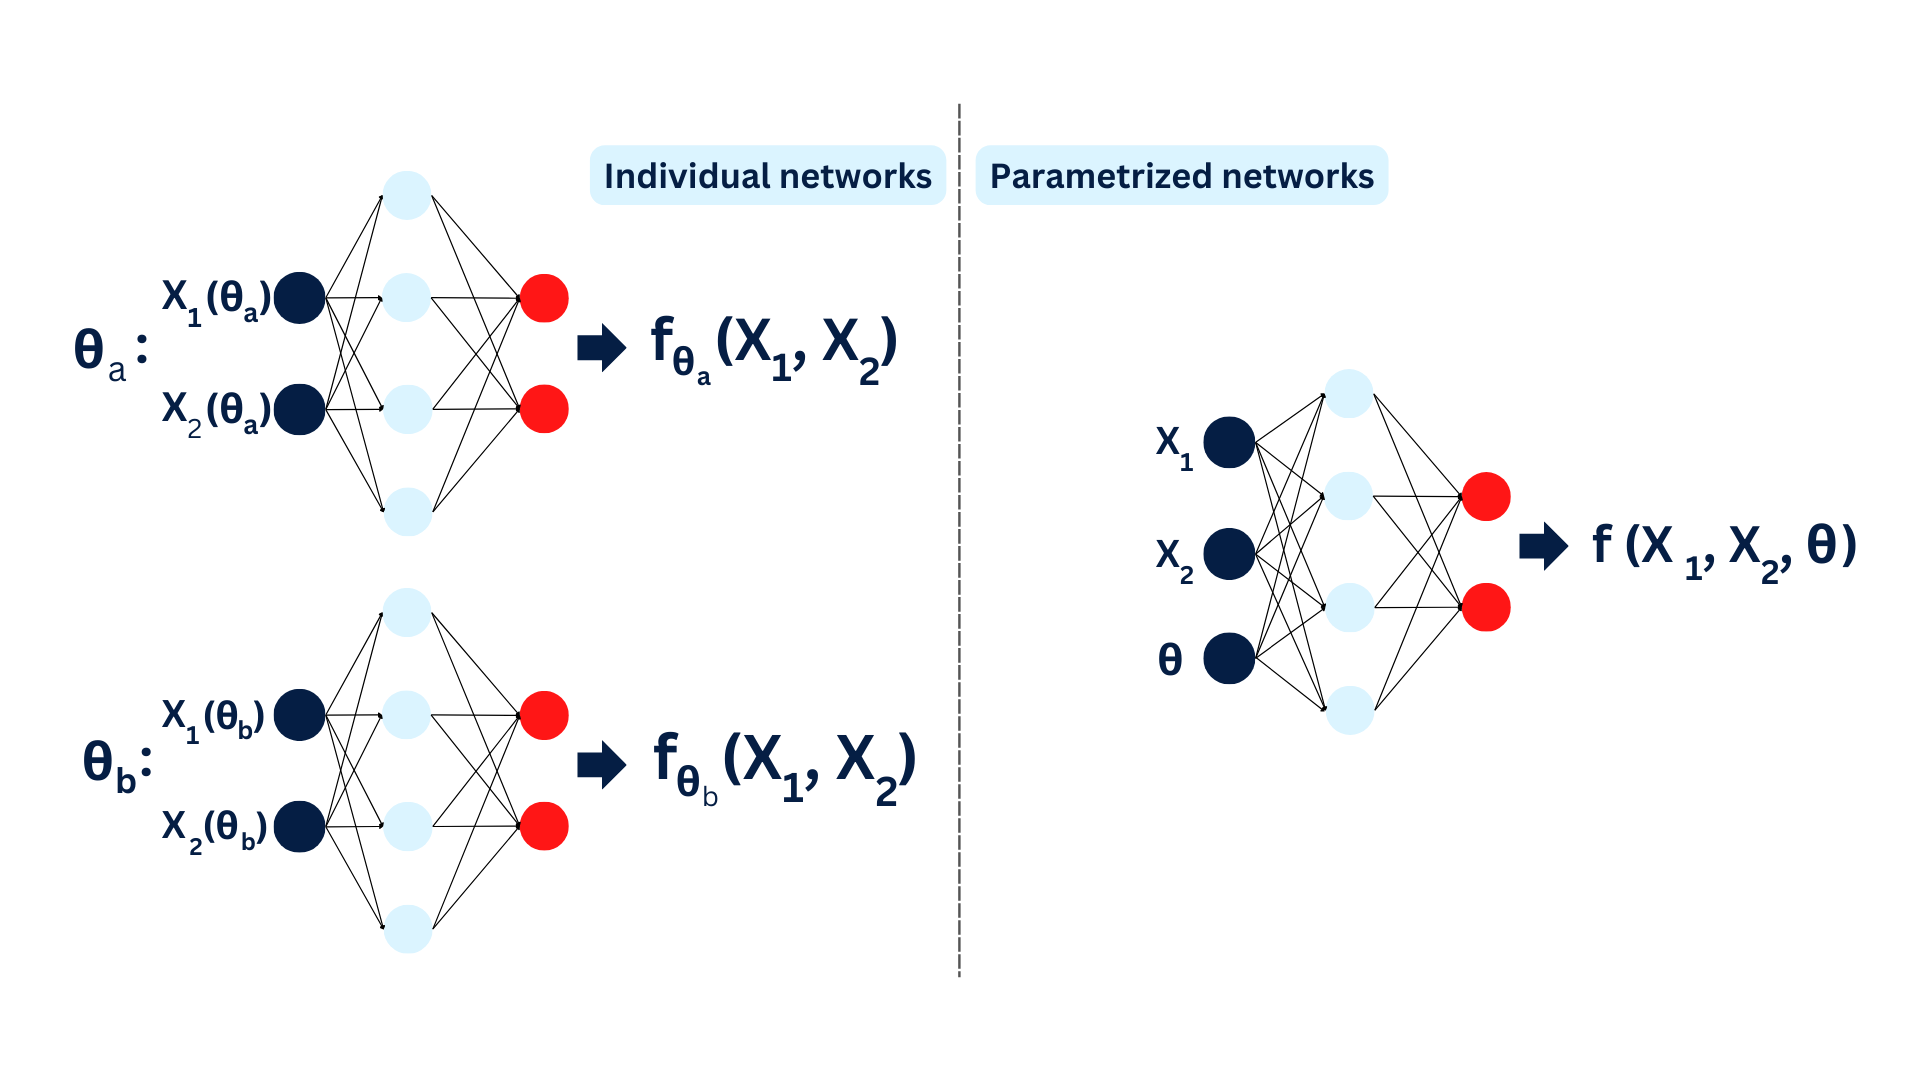
\includegraphics[width=0.8\textwidth]{Figures/Illustrations/PNN.png}
    \vspace{-.8cm}
    \caption{An illustration of a comparison between the parameter individualistic network 
    approach and the \acs{PNN}.}
    \label{fig:PNN}
\end{figure}
For the \ac{SM} background, adding a parameter representing the mass of a \ac{BSM} particle is meaningless. 
Therefore, the background is randomly assigned values according to the same distribution used in the signal data. 
In doing so, one is essentially assigning each set of signal its own portion of background data. 
\section{Decision Trees and Gradient Boosting}
\subsection{Decision Trees}
\ac{DT} are, similarly to \ac{NN} one of the most popular \ac{ML} methods used today.
Contrary to \ac{NN}, \ac{DT} are famously easy in theory. Despite the simplicity of \ac{DT}, 
they are capable of solving a large range of complex problems. In this section I will cover the use 
of \ac{DT} as applied to a supervised classification problem.
\\
The goal of decision trees are to create a flowchart-like tree structure from input to output. 
Similarly to the traditional cut-and-count method used in particle physics, a \ac{DT} 
places \emph{rectangular-cuts} on a data set. It does so to create a collection of thresholds 
$\bf{\mathcal{C}} \sf =\{c_1, c_2,...,c_{N_c}\}$, which when applied to a new data set and target, 
will sort each data point to the corresponding target. 
\\
In figure \ref{fig:DT}, I have illustrated a simple \ac{DT} classifying a 4-dimensional 
input data to one of three classifications. As is visualized in figure \ref{fig:DT}, the \ac{DT} 
applies a set of thresholds on the data to find the route applicable to a target. For each applied 
cut, the data split into what we call \emph{branches}. Each branch represents a subset of the data.
The final subset, after a sufficient amount of cuts ends in what we call \emph{leaves}. The leaves are 
the label we assign the subset of data contained in this branch.
\\  
\begin{figure}
    \centering
    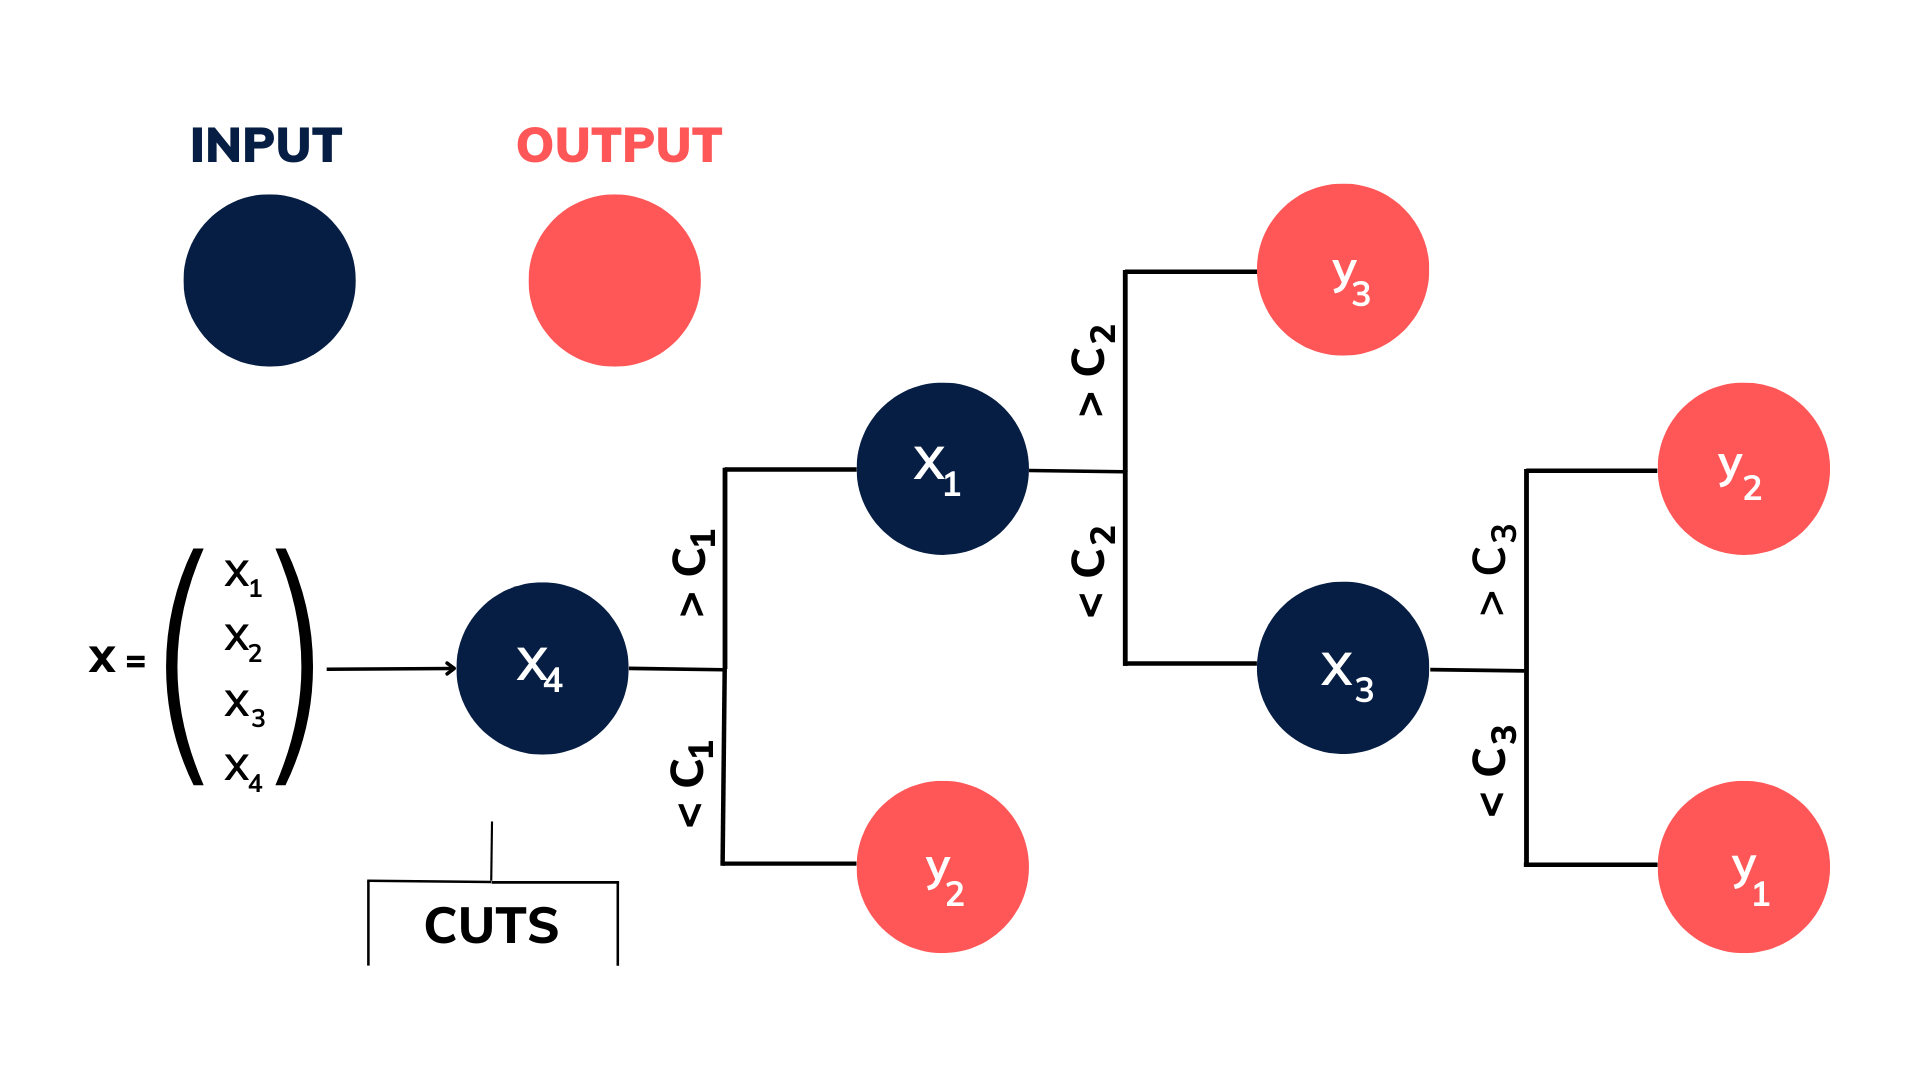
\includegraphics[width=0.6\textwidth]{Figures/Illustrations/DT.png}
    \caption{An illustration of a simple \ac{DT}, mapping a four dimensional input ($x_1,x_2,x_3,x_4$) 
    to one of three values in the target space ($y_1,y_2,y_3$).}
    \label{fig:DT}
\end{figure}
Just like most \ac{ML}-methods, there are many kinds of \ac{DT} each with their own 
architecture and benefits. In the case of \ac{DT} the defining qualities can be summarized in
its choice of \emph{Deepness} and \emph{Optimization}. When provided with a data set,
a \ac{DT} can in theory create as many cuts needed to map each individual data point, $\textbf{x}_i$ to the 
corresponding target, $t_i$. Doing so would not only be very computationally heavy, but would almost 
certainly lead to overfitting if applied to any new data. Instead, when building a \ac{DT} one defines 
a maximum deepness. This means that we must define a limit to the length of $\bf \mathcal{C}$, which 
subsequently leads to the need for a prioritization of cuts. 
\\
Building a \ac{DT} and choosing which cuts to apply at what point, is the equivalent of training a 
network. How to decide by what standard one chooses to building the hierarchy of cuts is again the 
equivalent of choosing an optimizer. For more information on \ac{DT}'s, the reader is referred to the 
book by Hastie et al. \cite{huang_introduction_2014}.
\subsection{Gradient Boosting in Decision Trees}
Gradient-boosting is an algorithm which uses a collective of "weak" 
classifiers in order to create one strong classifier. In the case of gradient-boosted 
trees the weak classifiers are a collective of shallow trees, which combine to form a classifier 
that allows for deeper learning. As is the case for most gradient-boosting 
techniques, the collecting of weak classifiers is an iterative process.
\\
We define an imperfect model $\mathcal{F}_m$, which is a collection of m number of weak 
classifiers, estimators. A prediction for the model on a given data-points, $\textbf{x}_i$ is 
defined as $\mathcal{F}_m(\textbf{x}_i)$, and the target for the aforementioned data is 
defined as $t_i$. The goal of the iterative process is to minimize some cost-function 
$\mathcal{C}$ by introducing a new estimator $h_m$ to compensate for any error, 
$\mathcal{C}(\mathcal{F}_m(\textbf{x}_i), y_i)$. In other words we define the new estimator as:
\begin{align}
    \tilde{\mathcal{C}}(\mathcal{F}_m(\textbf{x}_i), \textbf{y}_i) = h_m(\textbf{x}_i),
\end{align}
where we define $\tilde{\mathcal{C}}$ as some relation defined between the observed and 
predicted values such that when added to the initial prediction we minimize $\mathcal{C}$.
\\
Using our new estimator $h_m$, we can now define a new model as
\begin{align}
    \mathcal{F}_{m+1}(\textbf{x}_i) = \mathcal{F}_m + h_m (\textbf{x}_i).
\end{align}
Similarly to how we define a deepness of trees, we can define the degree of boosting. We define 
this as the amount of trees used in the iterative process, or M. This means that the final classifier 
becomes
\begin{align}
    \mathcal{F}_M (\textbf{x}_i) = \sum_{i=0}^M h_i(\textbf{x}_i)
\end{align} 
The XGBoost \cite{XGB} framework used in this analysis enables a (advanced) gradient-boosted algorithm, 
and was initially created for the Higgs ML challenge. Since the challenge, XGBoost has become 
a favorite for many in the ML community and has later won many other ML challenges. XGBoost 
often outperforms ordinary decision trees, but what is gains in results it looses in 
interpretability. A single tree can easily be analyzed and dissected, but when the number 
of trees increases this becomes harder. For more detailed explanation on the XGBoost framework,
the reader is referred to Ref.\cite{XGB}
\section{Machine Learning Applied to a BSM Search}\label{sec:MLHEP}
So far I have presented the goal of my analysis (to discover new physics)
as well as the tools I will be using to achieve it (\ac{ML}). In this section
I will discuss how \ac{ML} is applied to the problem as well as how it compares
to traditional methods.
\subsection{The Traditional Approach}
As discussed, I have been presented with two sets of data; the measured collision 
data from \ac{ATLAS} and the simulated \ac{MC} data. The origin of the latter data set 
will not be covered in great detail in this thesis, but it is worth mentioning that 
the simulations are based on \ac{SM} theory. In other words, by comparing the measured collision 
data with the \ac{SM} simulations, we are essentially comparing what is predicted by the \ac{SM} 
to what is measured by experiment. If the two differ in ways not explained by simulation error 
or other non physics related errors, one could interpret the deviation as new physics.
\\
In short, a search for new physics, is a search for deviations in the comparisons of simulations 
to experimental data. At first thought, this might seem like a simple task. Given that the deviations 
would be large, it would be easy. In reality, any new physics predicting large contributions 
in the data currently measured by \ac{ATLAS} has been excluded a long time ago. Today, any
promising extension of the \ac{SM} predicts to contribute rarely in any collision. As will 
be presented in later sections some theories that will be searched for in this thesis only 
contribute to a total of 6 collisions in a data set consisting of more than $3800000$ events 
($<0.002\%$). Not only would such a deviation be incredibly hard to detect, but it would 
be close to impossible to determine if such a deviation is rooted in new physics or simply 
noise. 
\\
The traditional approach to this problem is to study the data in physics motivated regions. 
For example, in section \ref{sec:signal} I presented the Feynman diagrams of the signals I 
searched for in this thesis. As mentioned, this type of final state is expected to exhibit 
large amounts of missing transverse energy\footnote{Due to the neutralions being both heavy, neutral 
and interacting only weakly with ordinary matter.}. The traditional approach is to neglect all the data 
with small amounts of missing energy, and only consider events of interest. By applying these kinds of 
constraints on the data, you are creating a region where you expect to find as much of the signal and as little 
of the background as possible. After applying a sufficient amount of demands (or cuts), you would count the 
remaining data in your \emph{search region} and check for deviation. This approach is called \acf{CC}.
\\
\begin{figure} 
    \centering
    \makebox[0.75\linewidth][c]{%
    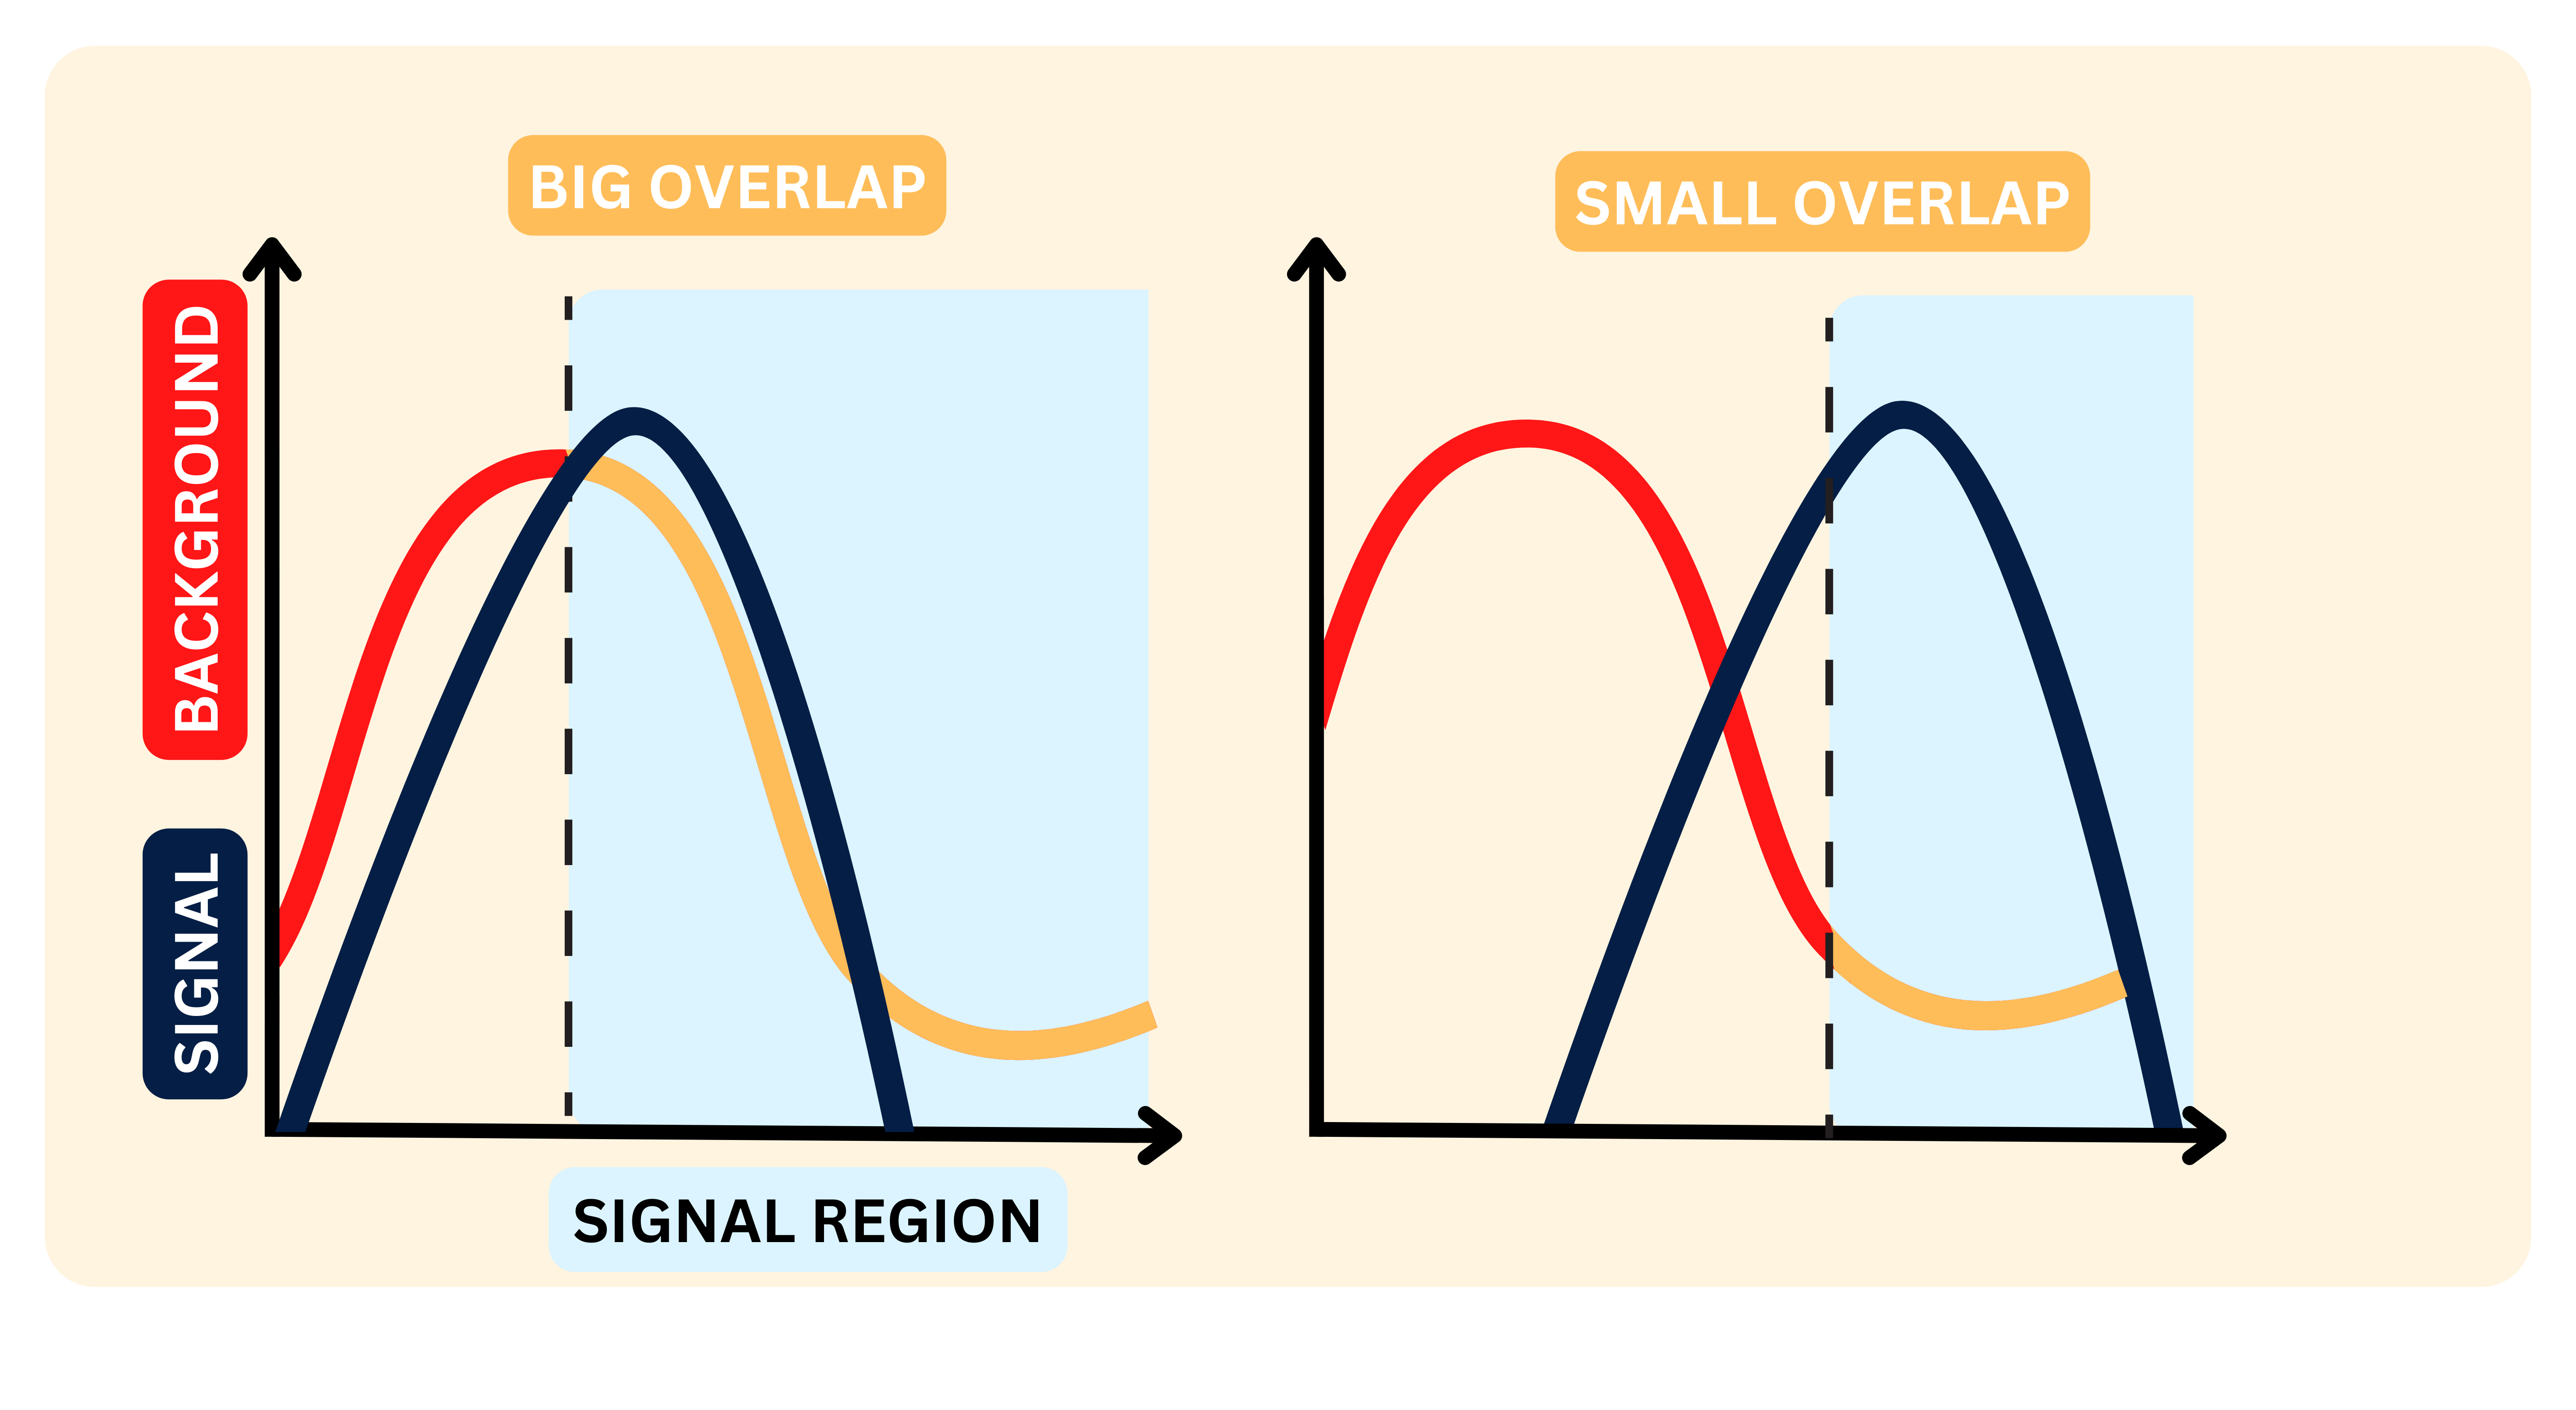
\includegraphics[width=0.65\textwidth]{Figures/Illustrations/CandC.png}
    }
    \caption{An illustration of a traditional \acf{CC} approach and how non-overlapping features lead to effective
    signal regions. In the first figure (left) the distributions of signal and background are relatively similar, and 
    the signal region contains large amounts of background. In the second (right), the distributions of signal and 
    background are greatly different, and this variable would allow for a much more effective signal region. }
    \label{fig:overlap}
\end{figure}
\subsection{The Machine Learning Approach}
For a signal which greatly differs from the \ac{SM}, the \ac{CC} method could be sufficient. But, in 
cases where the signal is similar to background, it becomes harder to create effective\footnote{By effective
cuts I mean cuts which removes large amounts of the background while at the same time preserves as much of 
the signal as possible.} cuts. In figure \ref{fig:overlap}, I have drawn an illustration of two different feature distributions both 
displaying the distribution for a hypothetical signal and background. Additionally, I have drawn a 
threshold in both distributions which represents the cut made to create a search region. In the first 
figure (left) the distributions of signal and background are relatively similar, and the signal region 
contains large amounts of background. In the second (right), the distributions of signal and background 
are greatly different, and this variable would allow for a much more effective signal region. 
\\
The goal of introducing \ac{ML}, is to create a new feature in the data set where background and signal
exhibit as little overlap as possible. This is very similar to how we introduce physics motivated high-level
features like invariant mass, but instead of using an analytical function grounded in physics, 
we apply the output of a trained \ac{ML} model. Then, once the \ac{ML}-variable is created, 
we apply a cut (similar to \ac{CC}) which will define an effective search region. 
\\
How we create the \ac{ML}-variable can vary depending on the type of \ac{ML}. In the case of unsupervised 
\ac{ML}, one aims to perform a type of anomaly detection. One unsupervised approach is to overfit on the background,
then hope that said overfitting is reflected when a new process is introduced. An effective unsupervised approach
would be incredibly beneficial, as it would be totally model independent. In other words, the same model could be applied 
to all signal. As mentioned in earlier sections (see section \ref{sec:MLPhen}), the focus of this thesis will not be on 
unsupervised \ac{ML}, but supervised. The largest difference between the two is the introduction of an additional data set,
the simulated signal. By simulating and training on what we expect the new physics to look like, we are able to achieve a much more 
effective output which is tailored to what we expect the new physics to look like. Though, what supervised learning gains in performance
it looses in generalizability, i.e. the ability to find new physics it has not trained on.
\section{Model Assessment}\label{subsec:Cost}
\subsection{The Rate of True-Positve - ROC Curve}\label{subsec:AUC}
A \ac{ROC} curve is a tool used to measure and visualize a binary classifiers' ability 
to predict trends. In figure \ref{fig:ROC} I have plotted an illustration of a \ac{ROC} curve.
The curve is plotted on an xy-axis where the x-axis represents 
false-positive rates and the y-axis represents true-positive. The different values 
for the curve are the rate of true positives with different thresholds, i.e. 
the value deciding whether an event is 1 or 0, signal or background. If a classifier 
has learned nothing and is simply guessing, the \ac{ROC} curve will be a linear curve 
going from 0 to 1. This line is often drawn in \ac{ROC} curve. The better the 
classifier is, the higher the \ac{ROC} curve will bend towards the upper-left corner of the 
graph. The closer the line is to the diagonal, the worse the classifier. 
\\
A metric often used to measure a classifiers' ability create an output which effectively 
separates two categories, is the \ac{AUC}. The larger the area, the better the separation. 
An ideal classifier which perfectly separates two categories will achieve a \ac{AUC} of 1.
A classifier which simply guesses, will achieve an \ac{AUC} of 0.5. Both this cases assume 
an equal weighting of both signal and background. 
\\
This present section was taken from some of my previous work, and can be found in the following 
rapport \cite{HirstFretteML}.
\begin{figure}
    \centering
    \makebox[0.75\linewidth][c]{%
    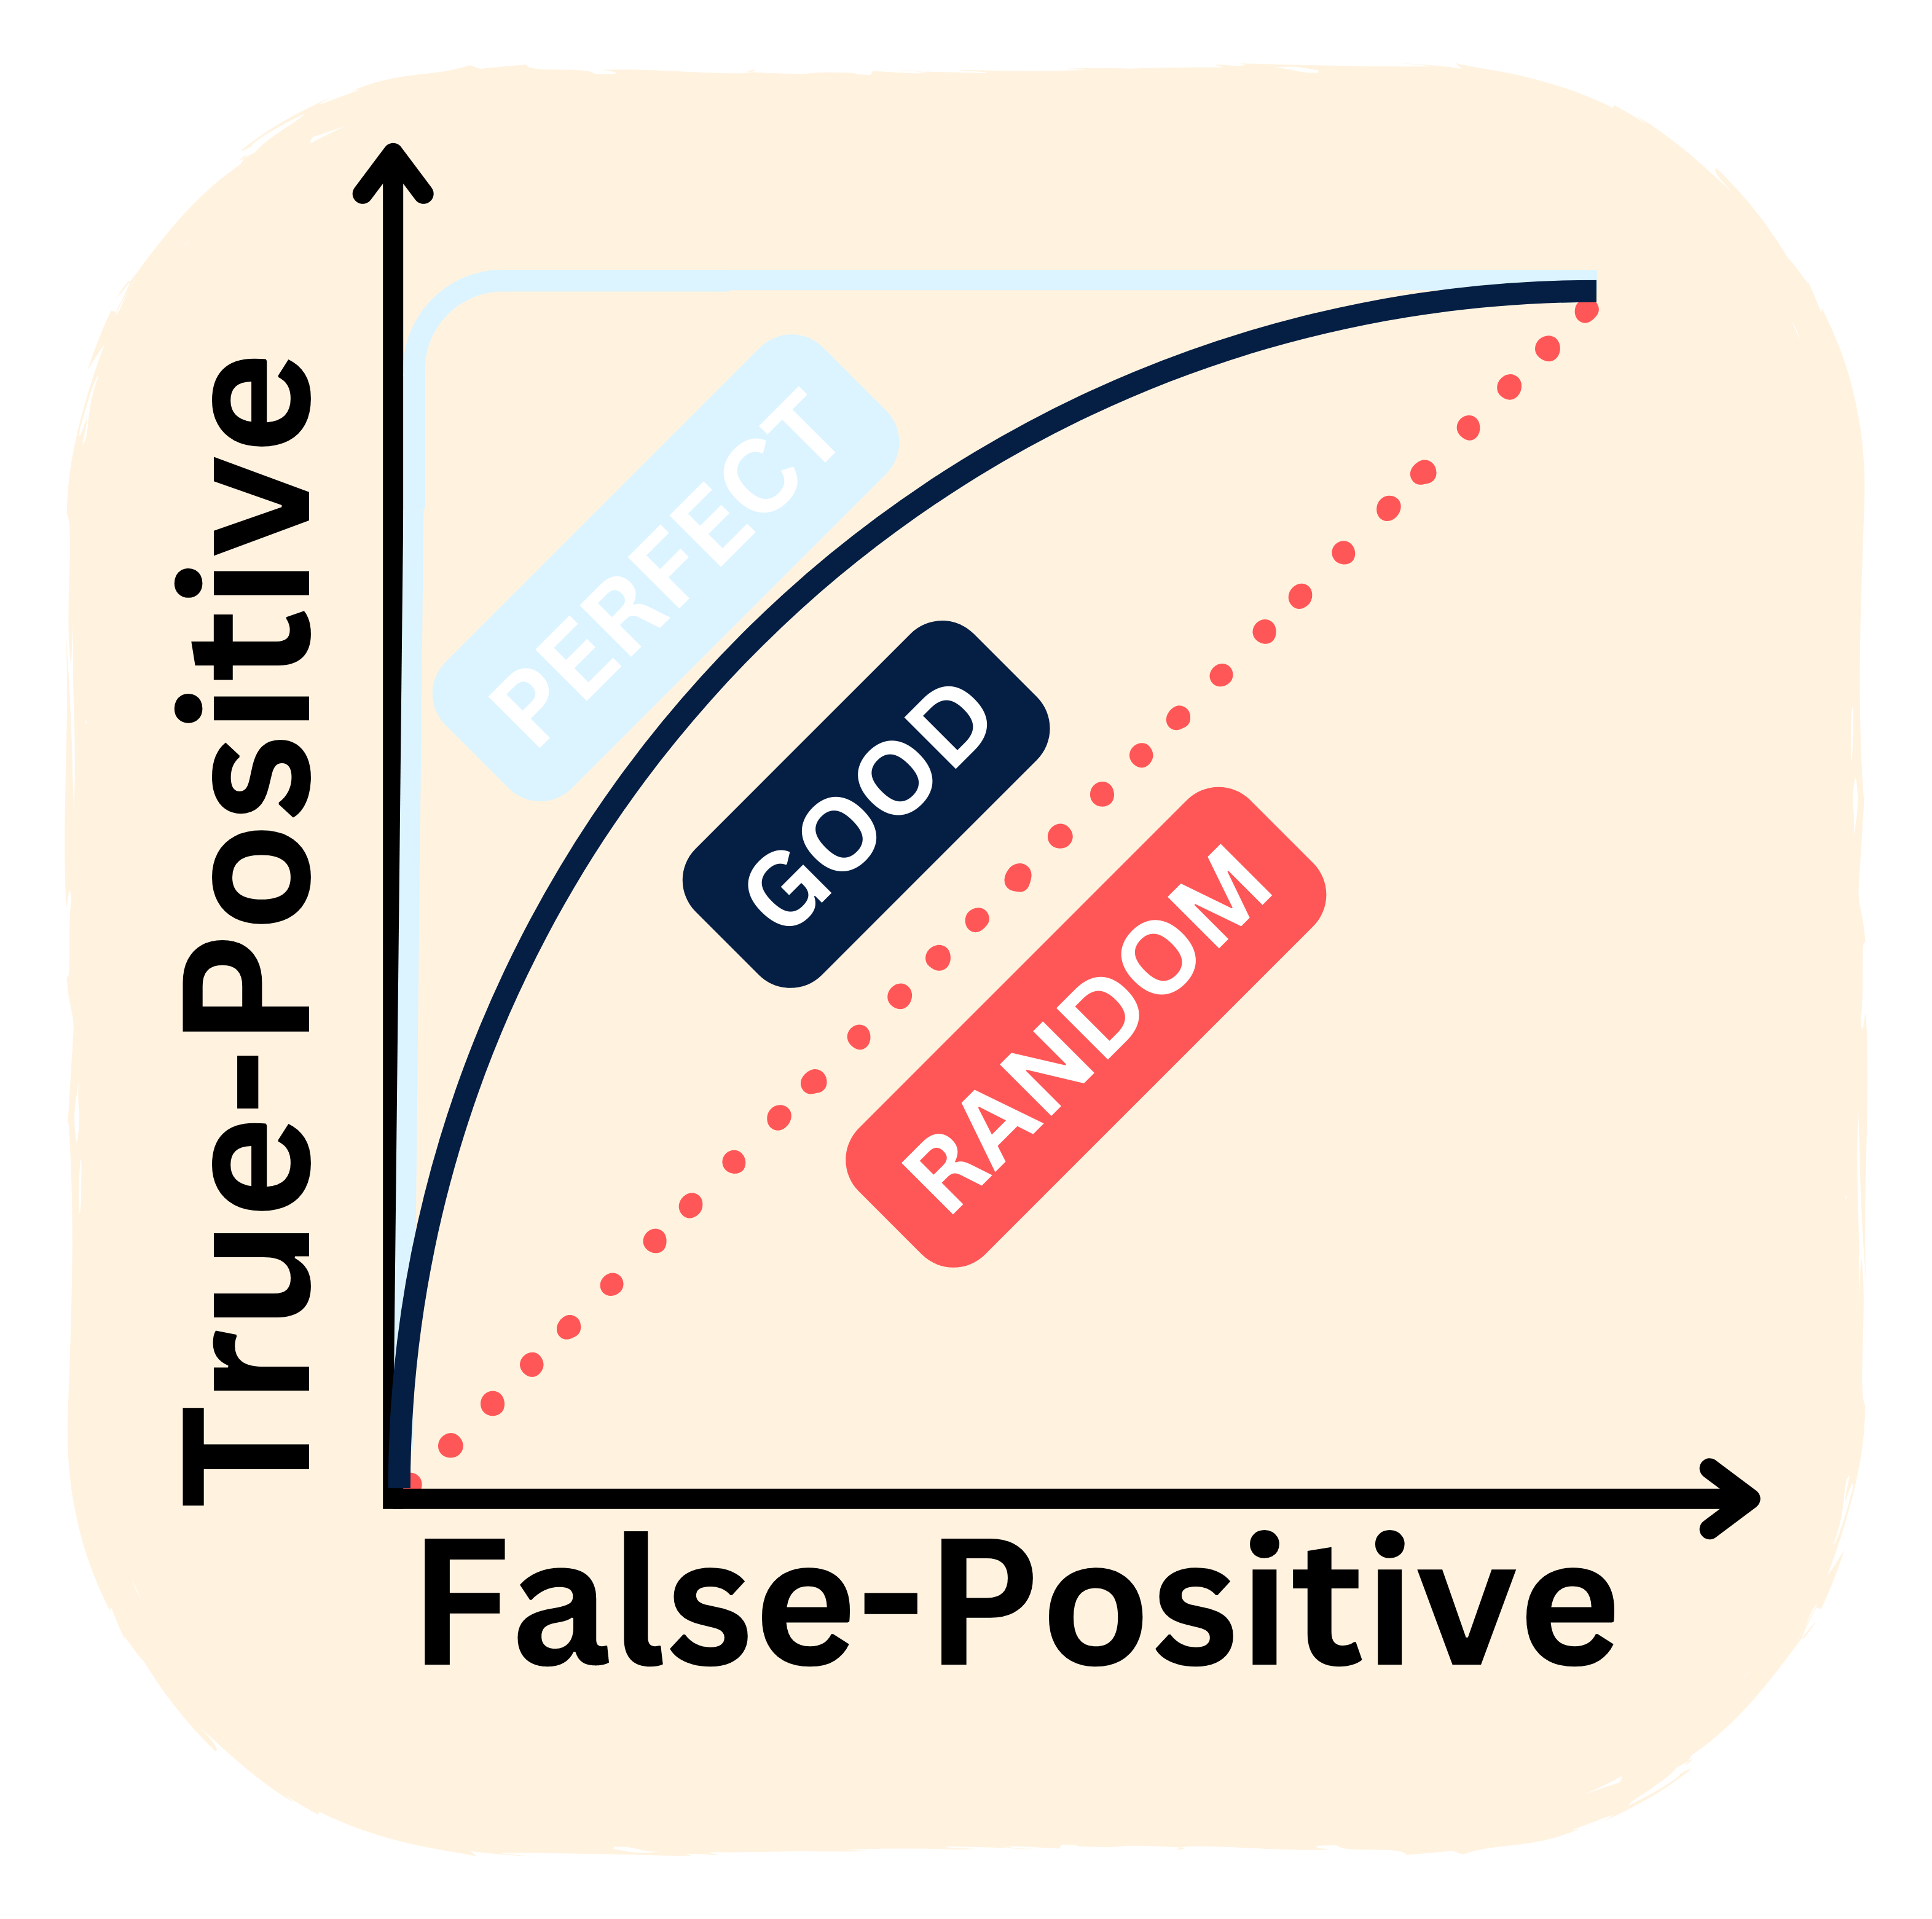
\includegraphics[width=0.45\textwidth]{Figures/Illustrations/True-Positive.png}
    }
    \caption{An illustration of a \acs{ROC} curve and how a random, good and perfect classifier would differ.}
    \label{fig:ROC}
\end{figure}
\subsection{Statistical Assessment - Discovery $\&$ Exclusion}\label{subsec:Sensitivity}
The statistical aspect of the analysis will not be of focus in this analysis, nonetheless there are 
some expressions which would be helpful to define. Let us assume that we expect to see no new physics in the collision
data, we can call this hypothesis the b(background)-hypothesis. To expect no new physics, is not the same as expecting no 
deviation. We still assume statistical uncertainties, or noise to effect the simulations which will affect the distribution of our 
simulations and lead to fluctuations. If these fluctuations are random, we can assume that the noise can be described by a Gaussian distribution 
(which is a good approximation for large statistics), which has a mean of 0 and a standard deviation equal to $\sqrt{b}$, where b is 
the number of \ac{SM} simulations. Using this assumption, we can state that the higher the deviation, i.e. the further away 
from the mean, the less likely such a deviation is explained by our b-hypothesis. Given a large enough deviation, we can even 
define the hypothesis as rejected with a certain confidence.
\\
We measure the deviation between the observed collision data and the simulated \ac{SM} data in units of significance, Z. 
For a given signal region with $n_{obs}$ events of measured collision data and b simulated \ac{SM} data, we define
the significance of a deviation as
\begin{align}\label{eq:Z1}
Z=\sqrt{2\left[n_{\text {obs }} \ln \frac{n_{\text {obs }}}{b}-n_{\mathrm{obs}}+b\right]} \text { or } 
Z=\sqrt{2\left[(s+b) \ln \left(1+\frac{s}{b}\right)-s\right]}, 
\end{align}
where we have defined the signal as $s = n_{obs} - b$. In the case of large statistics ($b>>s$), we can write Z 
as 
\begin{align}\label{eq:Z}
    Z=\frac{n_{o b s}-b}{\sqrt{b}} = \frac{s}{\sqrt{b}}.
\end{align}
By studying equation \ref{eq:Z} we observe that the significance of a deviation is simply the signal measured in units of standard
deviation of the Gaussian distribution. In physics, one often deems the results a discovery, or the b-hypothesis as rejected, if $Z>5$. 
\\
\begin{figure}[H]
    \centering
    \makebox[0.8\linewidth][c]{%
    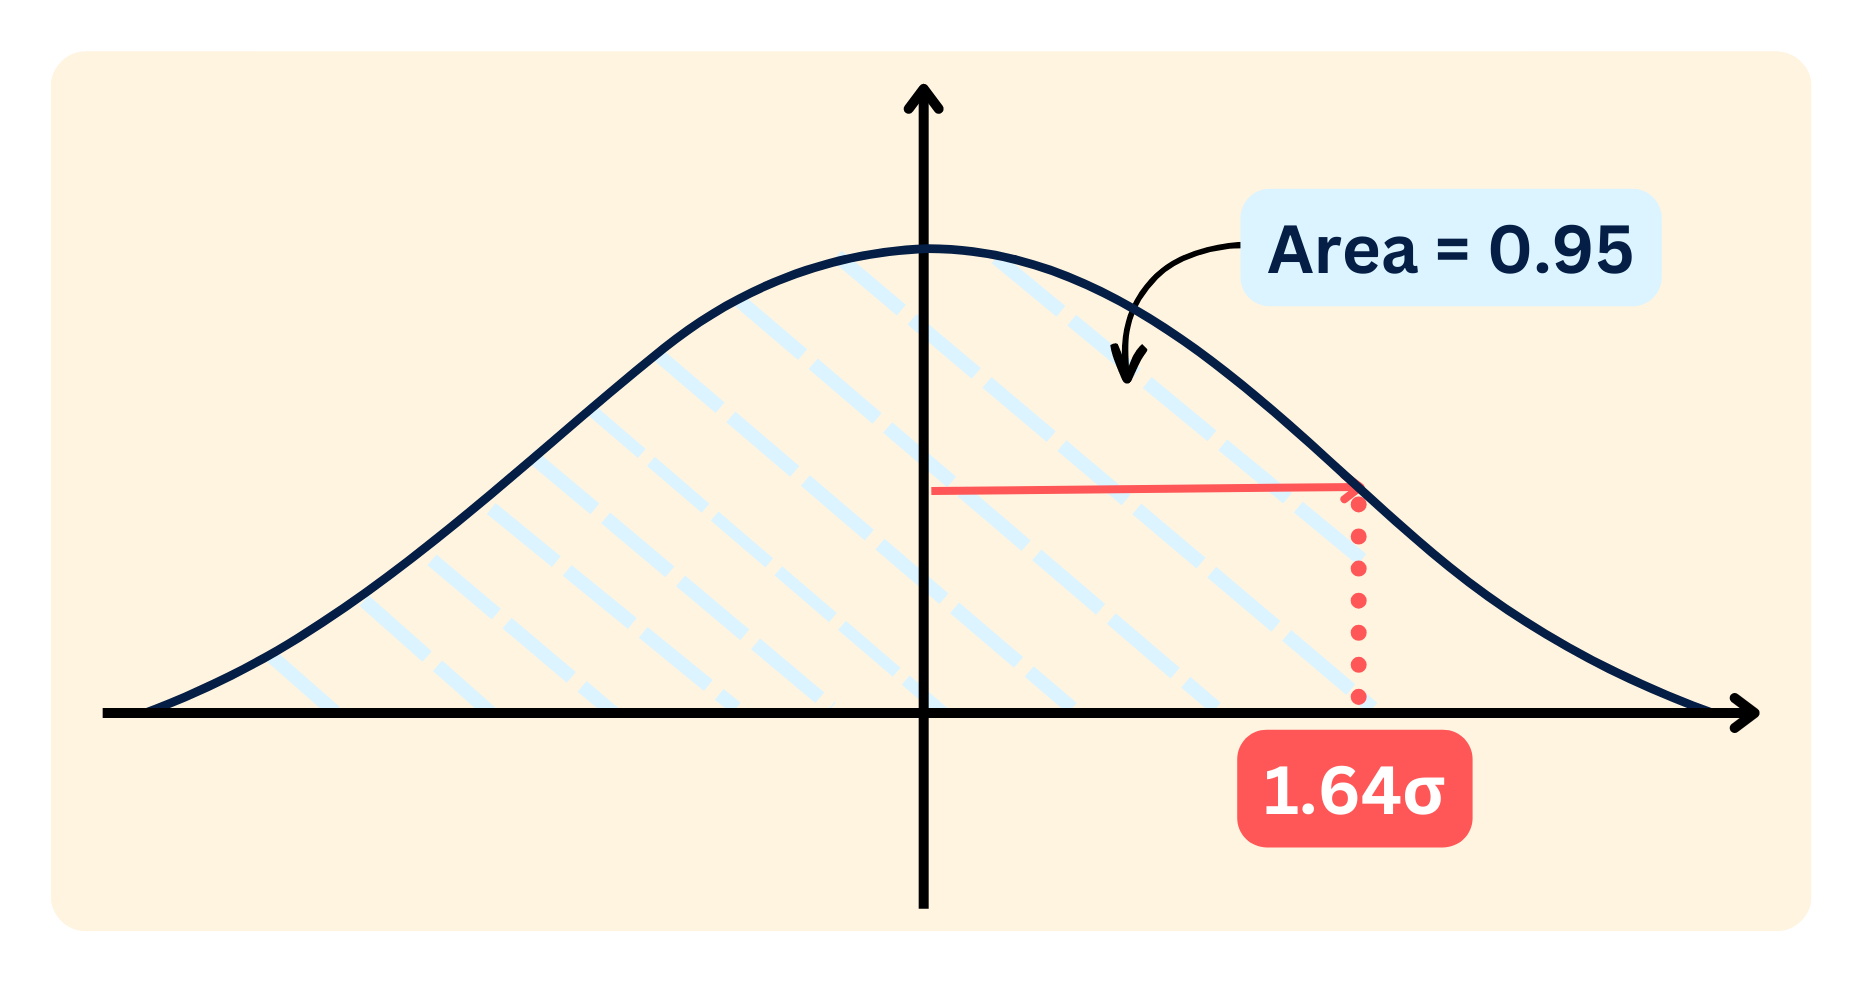
\includegraphics[width=0.45\textwidth]{Figures/Illustrations/ConfInt.png}
    }
    \caption{An illustration of a Gaussian distibution and the area under the curve defined by a significance equal to 1.64.}
    \label{fig:ConfInt}
\end{figure}
Before attempting to search for deviations in the real data, we are interested analysing the sensitivity of our method, as well 
as calculate the expected number of signal in our signal region. To study the sensitivity of an analysis one looks only at the 
simulated background and signal and performs a study to see how well one can separate background from signal. The measure of the sensitivity 
of our models will be of great focus in this thesis.
\\
In the case we are measuring the sensitivity, we do not have $n_{obs}$. Instead we simply define $s$ as the number of events of the simulated signal 
inside the signal region. This number would be spesific for each mass combination and will be a measure for how sensitive 
the model is for that exact combination. In physics, we define a model as sufficiently sensitive, if it is able to achieve a 
significance of 1.64. This number is chosen based on its relation to the b-hypothesis. A significance of 1.64, equals the 
distance from the mean of the Gaussian distibution which sums to an area of 0.95 (see figure \ref{fig:ConfInt}). There are many ways to inteprate this. A layman 
intepration (which is sufficient for this theisis), is that given the b-hypothesis is true, there is a $95\%$ probability that we will 
measure a signal which produces a significance of less than 1.64. Therefore, there is only a $10\%$ probability that the b-hypothesis
can explain the deviation. For more information on significance and discovery in physics the reader is reffered to the slides \cite{magnar}.


%%%%%%%%%%%% Implementation %%%%%%%%%%%%%%%%
\chapter{Introduction to supervised and unsuperised machine learning}\label{chap:Intro ML}
Machine learning is rapidly becomming an overwhelming presens in many different scientific fields.
In areas ranging from cancer research to stock-trading, machine learning is being applied to probelms
once thought as impossible to solve. Particle physics, like many other fields is no exeption. Jet flavor classification \cite{Guest_2016}, 
separating jets from gluons \cite{PhysRevD.44.2025} or using \ac{ML} to create efficent \ac{SR} are just some examples
where \ac{ML} is a vital tool. The traditional approach for ML in high-energy physics is through the use 
of supperivsed learning. \ac{DNN}


\section{The Simulated Data}
\subsection{Monte Carlo Simulated Data}
Up to this point in the thesis I have discussed two data sets: the measured collision data and the simulated \ac{MC} data. 
As far as my relation to the latter data set I have only used it directly in my analysis and have not been involved in 
production. The simulations applied in the creation of our simulated data set are all based on \acf{MC} simulations\footnote{For 
more information on \ac{MC} simulation, the reader is referred to \cite{raychaudhuri_introduction_2008}.}.
Through simulations, we are able to (among other things); test our understanding of the detector, model the expected \ac{SM} background 
events in different regions or model new \ac{BSM} physics. The pipeline for producing simulated events, closely mimic the pipeline 
from real collision to data set. The pipeline for simulating collision events can be summarized in the following steps
\begin{itemize}
  \item \emph{Generate events}: Simulate each event in the collision, marking each event with the corresponding process (see section \ref{sec:bkg})
  \item \emph{Simulate detection of events}: Simulate the detection of each event in the different layers of the detector described in section \ref{subsec:Detector}
  \item \emph{Digitization}: Translate the interaction between the particles in the events and the detector to real signals
  \item \emph{Reconstruct events}: Go through the same steps applied to real collisions to reconstruct particles from the detector output.
\end{itemize}
\subsection{The Simulated Signal}\label{subsec:signal}
As I have mentioned in previous sections I will be searching for a large range of signals, all related to the same
physics, but with different set of parameters, i.e. choices for the masses of the charginos and neutralino. In figure \ref{fig:nrSignal} I have drawn a 
grid displaying the different mass combinations searched for in this analysis. The masses range from ${\tilde{\chi}_1}\in[0,400]$GeV
and ${\tilde{\chi}_2}\in[200,800]$GeV\footnote{The chargino, $\tilde{\chi}^{\pm}_1$, and second neutralino, $\tilde{\chi}_2$, are mass degenerate, 
meaning they share the same mass. As a consequence, I will refer to the mass of each particle interchangeably throughout the thesis.}. In the beginning 
of my analysis I only received a subset (which will be referred to as the \emph{original} data set.) of the full signal set. In the figure I have marked the original data set with a white label in the top 
right corner of the box. The original signal set contains a total of 30 different mass combinations in the ranges 
${\tilde{\chi}_1}\in[0,400]$ and ${\tilde{\chi}_2}\in[400,800]$. In the full signal data set there are a total of 90 different 
mass combinations.
\\
Given that I received the original signal data set many months before receiving the full set, most of my results were carried out using the 
original set. Therefore, I choose to use the original data set to compare the performance of the models, then finally use the full set 
when comparing the results to previous analysis.
\begin{figure}
  \centering
  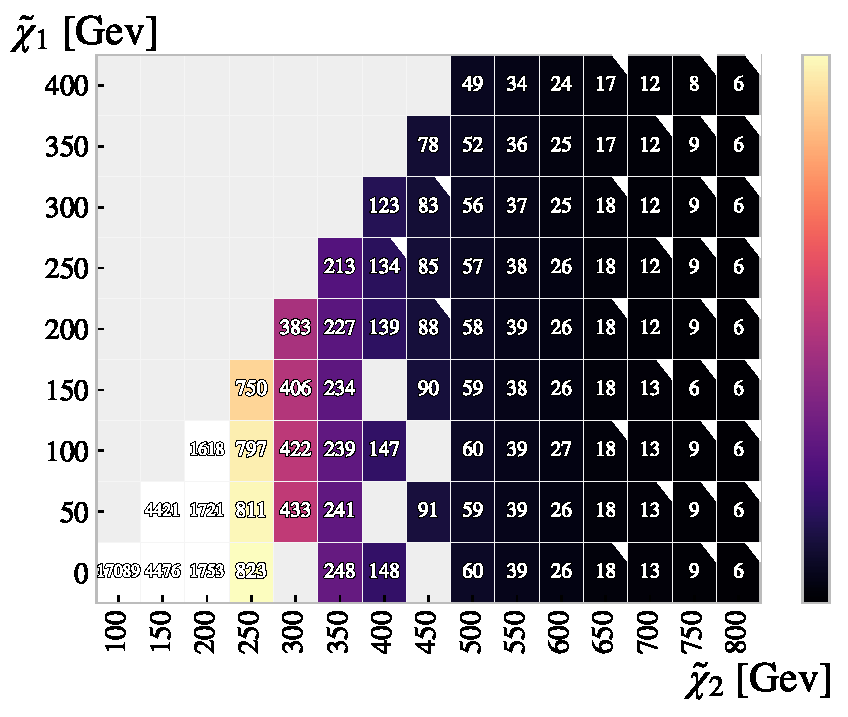
\includegraphics[width=0.85\textwidth]{Figures/MLResults/NN/SUSY/Grid/NrSignalEvents.pdf}
  \caption{A depiction of all mass combinations and their respective event count in the full signal data set.
  Additionally, a white corner has been added to all combinations which define the original signal set.}
  \label{fig:nrSignal}
\end{figure}
\section{The Tools}
Every year technology for generating and measuring particle collisions is improving. 
As a consequence, the amount of data increases drastically. The \ac{ATLAS} experiment
is one of the largest particle detector experiments currently operating at the 
CERN laboratory near Geneva. \ac{ATLAS} alone generates approximately 1 petabyte of raw
data every second from proton-proton collisions at the \ac{LHC}. In this analysis I will 
be studying proton-proton collisions at a center of mass energy $\sqrt(s) = 13$TeV recorded by \ac{ATLAS} detector 
between 2015-2018, corresponding to an integrated luminosity of $139.0fb^{-1}$. With amounts of data this large, 
data handling and storing is a big challenge. Therefore, taking advantage of sophisticated numerical tools 
and data frameworks is pivotal if scientific development is to keep up with technological development.
\subsection{ROOT}
In many aspects of my analysis, ranging from statistical analysis to plotting I utilize the \verb!ROOT! framework.
\verb!ROOT! \cite{ROOT} is at its core a large $\verb!C++!$ library and data structure made specifically for big data
analysis and computing, as well as data visualization. Today, all \ac{ATLAS} data is stored as ROOT-files, 
summing up to more than 1 exabyte ($10^{12}$) distributed worldwide through the World \ac{LHC} Computing Grid (WLCG)\cite{bird_update_2014}. 
\verb!ROOT! has many \ac{HPC} qualities which makes it ideal for particle physics analysis which demands heavy computations. Additionally, 
many particle physics-specific packages have been developed to make it an even better tool. Any function not already in library,
can easily be added in a \ac{HPC}-effective manner through $\verb!C++!$.
\\
Many of the plots presented in the present thesis were created using \verb!ROOT!. \verb!ROOT! has implemented a highly intuitive and
effective \ac{API} for data comparison and visualization. \verb!ROOT! allows for quick and direct 
comparison between data through an advanced graphical user interface. Furthermore, a lot of
functionality for creating complex stacked histograms are implemented in the \verb!ROOT! \ac{API}, such
as uncertainty calculations, ordering of histograms and statistical analysis tools. A final and important benefit of 
\verb!ROOT! is its impressive handling of memory which makes it ideal to handle large amounts of data.
\subsection{Data Structure and Frameworks}
Both data sets used as input to the analysis in this thesis, the measured and simulated, were stored in \verb!ROOT!, in the format of \verb!NTuples!. 
\verb!NTuples! are \verb!ROOT! objects designed to store large amounts of data. They allow for non-symmetrical entries, meaning 
rows with different number of columns. The simulated and measured collision data are both stored in \verb!NTuples!, with a matrix like structure 
where the columns represent the variables/features, and the rows represent each event. Hence, allowing non-symmetrical entries is essential 
for the purpose of storing data on particle collisions, given that not all variables are relevant for all events. For example the $P_t$ of the 
third lepton in an event in a two lepton final state, does not make sense.
\\
When starting preprocessing I load the \verb!NTuples! using a \verb!ROOT! interface called \verb!RDataFrame!\footnote{For full 
documentation on RDataFrame, see $\href{https://root.cern/doc/master/classROOT\_1\_1RDataFrame.html}{https://root.cern/doc/master/classROOT\_1\_1RDataFrame.html}$ 
(Accessed 16.04.2023).}. \verb!RDataFrame! allows for easy addition of new columns as well as filtering of events through native functionality. 
As a consequence I used \verb!RDataFrame! to calculate all features not already in the data set, such as the sum of transverse momentum, 
or the invariant mass of the three leptons. 
\\
After pre-processing was completed, I used \verb!RDataFrame!'s \emph{AsNumpy} function to translate the data frame into 
\verb!Numpy! objects, which then allowed me to transform it to a \verb!Pandas! data frame \cite{Pandas}. This is done
because \verb!Pandas!, like most \ac{ML}-tools, work in a strict \verb!Python! environment. \verb!Pandas!, similarly to \verb!RDataFrame!,
includes a deep computational library, and is optimal for analysis of big data. When the full \ac{ML} 
pipeline (data-handling, training, validation etc.) is completed the data is transformed back to \verb!NTuples!, 
to take advantage of the plotting functionality in \verb!ROOT!. The workflow of the data pre-processing is visualized in figure 
\ref{fig:WF}.
\begin{figure}
  \centering
  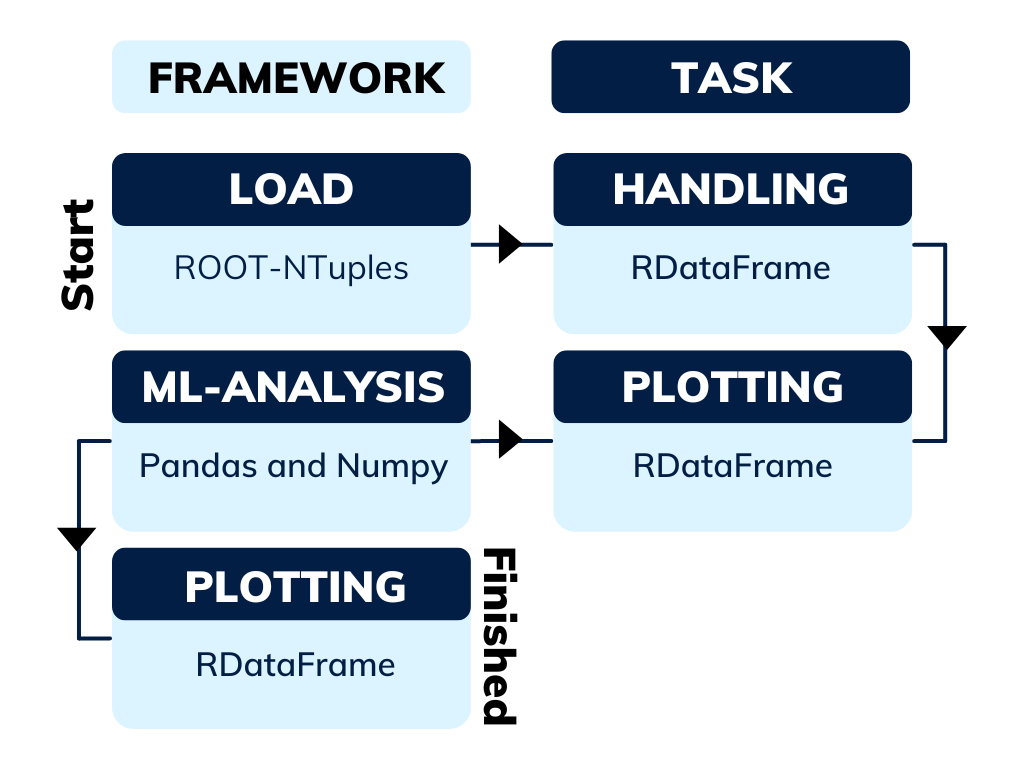
\includegraphics[width=0.7\textwidth]{Figures/Illustrations/TaskFlow.png}
  \vspace{-1cm}
  \caption{A visual summary of the workflow and frameworks used in the 
  computational analysis. }
  \label{fig:WF}
\end{figure}
\subsection{Computing Features in ROOT: Example}
In this section I will cover a simple example to highlight the steps taken in preparing the data set 
used in the analysis. As mentioned earlier, the two main frameworks used were \verb!RDataFrame! and \verb!Pandas!. 
In this example I will cover the case of a feature not already in the \verb!ROOT! file, namely the trilepton
invariant mass. All loading of data is done using the \verb!ROOT! framework and is easily read using the
\verb!RDataFrame! interface. To effectively generate new features we want to stay in \verb!ROOT! environment. Therefore,
we create a \verb!C++! file, \texttt{helperfunction}. The \texttt{helperfunction} contains additional 
\verb!ROOT! functions which are used in the analysis and are not already native to \verb!ROOT!. In the case 
of computing the trilepton invariant mass, the \verb!C++! function is created like shown in listing 
\ref{lst:mlll}.
\\
In listing \ref{lst:mlll}, we see a couple of measures taken to uphold to the \verb!ROOT! environment. The first measure is 
the typecasting to $VecF\_t$. $VecF\_t$ is created to wrap floats in the native \verb!ROOT! vector object, $RVec$. 
The same is done in other cases such as float and integers, $VecI\_t$ and $VecB\_t$. The second measure
was using \verb!TLorentzVector! \footnote{For full documentation on TLorentzVector, see $\href{https://root.cern.ch/doc/master/classTLorentzVector.html}{https://root.cern.ch/doc/master/classTLorentzVector.html}$ (Accessed 16.04.2023).} 
to calculate the invariant mass. \verb!TLorentzVector! is a class native to \verb!ROOT! with many built-in functions. In 
this case we use the class to create four-vectors through the kinematic variables, $P_t$, $\eta$, $\phi$ and mass\footnote{These features
will be described in the next section \ref{sec:Feats}.}. Then, through the \verb!TLorentzVector! class we can simply add, through vector sums, 
together and extract the invariant mass of the three-lepton system. 
\lstset{style=Cpp}
\begin{lstlisting}[caption={$C{++}$-function which implementes the calculation of $M_{lll}$.},captionpos=b, label={lst:mlll}]
// Compute the trilepton invariant mass 
float ComputeInvariantMass(VecF_t& pt, VecF_t& eta, VecF_t& phi, VecF_t& m) {
  TLorentzVector p1;
  TLorentzVector p2;
  TLorentzVector p3;
  p1.SetPtEtaPhiM(pt[0], eta[0], phi[0], m[0]);
  p2.SetPtEtaPhiM(pt[1], eta[1], phi[1], m[1]);
  p3.SetPtEtaPhiM(pt[2], eta[2], phi[2], m[2]);
  return (p1 + p2 + p3).M();
}
\end{lstlisting}
The functions implemented in the \verb!C++! library (\texttt{helperfunction}) off-loads, from \verb!Python!, all the time, consuming work to \verb!C++!,
which significantly speeds up the computation. The \verb!C++! library is compiled prior to the execution of the main \verb!Python!-code, which 
will be presented in the following. The main code, doing the selections, calculations and plotting, uses the \verb!RDataFrame! interface in a \verb!Python! 
environment. Whenever heavy calculations are needed the \verb!RDataFrame! interface calls on function in the \verb!C++! library described above. 
\\
In the code written in listing \ref{lst:df_mlll}, I show a simple example 
of loading new \verb!C++! functions, filtering out events, calculating new features and adding said 
features to a histogram. The first three lines of code both compiles and include the \texttt{helperfunction} 
into the \verb!ROOT! framework. Then I loop over all keys in the data frame, which in my case
are the different channels (i.e diboson, $t\bar{t}$ etc.). For each channel I select 'good' events,
based on the criteria I will present in section \ref{subsec:Cuts}. Then I use \verb!RDataFrame!'s \texttt{Define} function to calculate
and add a new feature using the \texttt{ComputeInvariantMass}-function. Finally, I save the feature as \verb!ROOT! object called 
\texttt{Histo1D}, which I later plot using \verb!ROOT! \ac{API}. In this example I chose the trilepton invariant mass, 
but in the analysis all additional features were calculated using a similar method. 
\lstset{style=Python}
\begin{lstlisting}[caption={Python-file for calling dataframe and calculating $M_{lll}$.},captionpos=b, label={lst:df_mlll}]
R.gROOT.ProcessLine(".L helperFunctions.cxx+");
R.gInterpreter.Declare('#include "helperFunctions.h"') 
R.gSystem.Load("helperFunctions_cxx.so")

for k in df.keys():
    # Define good leptons
    isGoodLepton = "feature1 < cut1 && feature2 >= cut2"

    # Define good leptons in dataframe
    df[k] = df[k].Define("isGoodLepton",isGoodLepton)

    # Define number of good leptons
    df[k] = df[k].Define("nGoodLeptons","ROOT::VecOps::Sum(isGoodLepton)")

    # Demand 3 good leptons 
    df[k] = df[k].Filter("nGoodLeptons == 3")

    # Define Invariant Mass (lll)
    df[k] = df[k].Define("mlll","ComputeInvariantMass(lepPt[isGoodLepton], 
                                                      lepEta[isGoodLepton], 
                                                      lepPhi[isGoodLepton], 
                                                      lepM[isGoodLepton])")
    # Add to histogram
    histo["mlll_%s"%k] = df[k].Histo1D(("mlll_%s"%k,
                                        "mlll_%s"%k,40,50,500),
                                        "mlll",
                                        "wgt_SG")     
\end{lstlisting}




\section{Features - Selection and Preprocessing}
The choice of which features to study and which to neglect is crucial in a search for new physics. This is particularly true 
in the case of applying machine learning. The general motivation for including a given feature can be based on several factors. 
The first being its ability to provide a trend which we as researchers can exploit when creating ours signal search regions. By this I mean
that it is a variable were there is diversity in distribution between the different channels. The second motivation is grounded in 
physics. Often we as physicists tend to lean towards variables we know have some effect one the physics we are studying. For 
example the missing transverse energy, $E_T^{miss}$ can be directly used to either include or discard events were we do or do not expect final states
with sufficient missing energy. The final motivation is grounded in the \ac{MC}-simmulations ability to represent the variable.
If there seems to be a clear deviation between the real and \ac{MC}-data which does not stem from any new physics, we tend to discard
them from the analysis.
\section{Data Preprocessing and Preselection Cuts}\label{subsec:Cuts}
To allow for deep learning and a thorough analysis one must try and keep
as much of the data as possible. At the same time, including large amounts
of irrelevant data can be both redundant and destructive\footnote{By including 
large amounts of irrelevant data, you risk the \ac{ML}-model tuning unnecessarily 
to remove easily reducible background, which could compromise performance.}. 
Therefore, preprocessing in the form of preselection cuts are necessary. 
The cuts applied in the analysis were grouped in two definitions, baseline and signal. 
The baseline requirements are written in table \ref{table:BL} and the signal requirements are written 
in table \ref{table:SG}. Both sets of requirements were taken from the \ac{ATLAS} article from 2022 \cite{franchini_search_2019}.
Given the definitions we demand that each event contains exactly three signal (\ref{table:SG}) and 
three baseline leptons (\ref{table:BL}), thereby removing any event with more or less. 
\\
Leptons are identified in the detector by using a likelihood-based method combining
information from different parts of the detector. The criteria of Loose or Tight 
identification are simply different thresholds in the discriminant, where Loose is 
defined as a lower threshold than Tight \cite{Aaboud_2019}. The overlap removal is used to solve any cases
where the same lepton has been reconstructed as both a muon and an electron. The boolean
of $lepPassOr$ simply applies a set of requirements to avoid any double counting. The cut for
the longitudinal track parameters, $z_0$ is applied to ensure that the leptons originate from the 
primary vertex.
\\
As for the requirements for the signal leptons, we require all baseline requirements are passed 
with the addition of a few more. We require Loose isolation for both electrons and muons. This means
requiring isolation criteria for a cone around the lepton is used to suppress \ac{QCD}-background events
and reduce fake leptons. Similarly to the $z_0$-cut, the transverse track parameter is also used to ensure 
origin from primary vertex.
\begin{figure}[H]
    \renewcommand\figurename{Table}
    \centering
    \footnotesize
    \makebox[\linewidth][c]{
        \begin{subfigure}{.475\textwidth}
            $
            \begin{array}{ccc}
                \hline \text { Requirement } & \text { Baseline electrons } & \text { Baseline muons } \\
                \hline\text{Identification} & - & \text{Loose} \\
                \text { Overlap Removal } & \text{lepPassOR} & \text{lepPassOR} \\
                \eta-\text { cut } & |\eta|<2.47 & |\eta|<2.7  \\
                \left|z_0 \sin (\theta)\right| \text { cut } & \left|z_0 \sin (\theta)\right|<0.5 \mathrm{~mm} & \left|z_0 \sin (\theta)\right|<0.5 \mathrm{~mm} \\
                \hline
            \end{array}
            $
            \caption{}
            \label{table:BL}
        \end{subfigure}
        \hspace{1.cm}
        \begin{subfigure}{.475\textwidth}
            $
            \begin{array}{ccc}
                \hline \text { Requirement } & \text { Signal electrons } & \text { Signal muons } \\
                \hline\text{Baseline} & \text{yes} & \text{yes} \\
                \text{Identification} & \text{Tight} & - \\
                \text{Isolation} & \text{LooseVarRad} & \text{LooseVarRad}  \\
                \left|d_0\right| / \sigma_{d_0} \text { cut } & \left|d_0\right| / \sigma_{d_0}<5.0 & \left|d_0\right| / \sigma_{d_0}<3.0 \\
                \hline
            \end{array}
            $
            \caption{}
            \label{table:SG}
        \end{subfigure}
        
    }
    \caption{Two tables displaying the baseline \ref{table:BL} and signal \ref{table:SG} requirements applied 
    to the data as part of the preprocessing.}
\end{figure}
In addition to the simple cuts, we must insure a good comparison between
\ac{MC}- and real data. Often one finds large deviation between the two in the case
of either very large or very small transverse momentum, $P_t$. The latter case can often be caused by 
poor reconstruction or miss identification. These are issues we aim to solve by checking
different triggers. 
\\
In the earlier parts of the analysis, I discovered that the data set I was given, did not contain the correct information 
regarding the triggers. After spending some time trying to compensate for this, my supervisor (Eirik Gramstad) suggested an alternative.
Instead of filtering using the triggers, an additional criterion of at least two leptons containing $P_t>20$GeV was placed on the data,
as it was suggested that this would be relatively equivalent.
% Given our data set is composed of different data sets spread over
% several years, different triggers are used. 
% \begin{table}
%     \centering
%     $
%     \begin{array}{ccc}
%         \hline \text { 2015 } & \text { 2016 } & \text { 2017 + 2018 } \\
%         \hline
%         \text{HLT\_2e12\_lhloose\_L12EM10VH} & \text{HLT\_2e17\_lhvloose\_nod0} & \text{HLT\_2e17\_lhvloose\_nod0\_L12EM15VHI} \\
%         \text{HLT\_e17\_lhloose\_mu14} & \text{HLT\_e17\_lhloose\_nod0\_mu14} & \text{HLT\_e17\_lhloose\_nod0\_mu14} \\
%         \text{HLT\_mu18\_mu8noL1} & \text{HLT\_mu22\_mu8noL1} & \text{HLT\_mu22\_mu8noL1} \\
%         & & \text{ HLT\_2e24\_lhvloose\_nod0}\\

%         \hline
%     \end{array}
%     $
%     \caption{Trigger requirments for events produced in their respective years.}
% \label{table:Triggers}
% \end{table}

\subsection{Lepton Variables}\label{subsec:LepSel}
Information regarding the kinematics of the electrons and muons were added into the data set: i.e. the transverse momentum, $p_T$, the pseudo 
rapidity $\eta$ and the azimuth angle $\phi$. All kinematic features were represented individually for each lepton. For example $p_T$
was added as three columns, $p_T(l_1)$, $p_T(l_2)$ and $p_T(l_3)$, where the ordering of the leptons were based on the momentum from highest ($l_1$) to lowest ($l_3$).
Similarly, I added information regarding the charge ($\pm$) and flavor (electron, muon) of each lepton. Based on the kinematic variables
the transverse mass $M_T$ of each lepton was calculated, $\Delta R$ and the transverse component, $E_T^{miss}$, and azimuth angle, $\phi^{miss}$,
of the missing momentum.
\\
Furthermore, I added different mass variables, namely $m_{lll}$ and $m_{ll}(OSSF)$ (\ac{OSSF}). The first being the trilepton invariant mass 
and the latter being the dilepton invariant mass of the pair with \ac{OSSF}. In the case of more than one possible \ac{OSSF}-pair,
the pair with the highest invariant mass was chosen. Secondly I added variables composed of the sum of the transverse momenta.
These variables include the sum of the transverse momenta of all three leptons, $H_T(lll)$, of the same sign lepton pair, $H_T(SS)$, and the sum of 
the momentum for all three leptons added with the missing transverse energy $H_T(lll) + E_T^{miss}$. Finally, I added the significance of the
$E_T^{miss}$, $S(E_T^{miss})$. The $S(E_T^{miss})$ is based on the log-likelihood ratio which compares the reconstructed $E_T^{miss}$ to 
the expected missing transverse energy in the case that there is no $E_T^{miss}$. For more information on $S(E_T^{miss})$ the reader is 
referred to \cite{object_based_2018}.
\subsection{Jet Variables}\label{subsec:JetSel}
Now we can have a look at the jet-features. Given that the final state of interest should be independent of jets, there are 
not many features added with jet information. But, given the risk of mis-identification, some jet features were included. The 
first features added were the number of jets, both all signal\footnote{See section \ref{subsec:Cuts}.} jets and number of b-jets.
The latter information was divided in two columns based on the efficiency of a multivariate analysis used to separate jet-flavors.
The efficiencies used for b-tagging are $77\%$ and $85\%$. The last information added for the jets were the mass of the leading pair 
(based on $p_t$) di-jet mass, $m_{jj}$.

\subsection*{Validation}\label{subsec:Validation}
As mentioned in previous sections, the comparison between \ac{SM} \ac{MC} and real data is a crucial part of the analysis, 
and we must therefore insure an adequate reconstruction of the real data before we begin the analysis. This is not only 
true for the low-level features, but for all features used in the analysis to create a new \ac{ML} variable. Therefore, 
we will in this section compare both sets of data for all features included in the analysis.
\begin{figure}[H]
    \renewcommand\figurename{Table}
    \centering
    \makebox[0.6\linewidth][c]{%
        \begin{subfigure}{.3\textwidth}
            $
            \begin{array}{cccc}
                \hline \text { Feature } & \text { $l_1$ } & \text { $l_2$ } & \text { $l_3$ } \\
                \hline\hline\text{$p_t$} & - & \ref{fig:lep2_Pt} & \ref{fig:lep3_Pt}\\
                \text{$\eta$} & - & \ref{fig:lep2_Eta} & \ref{fig:lep3_Eta}\\
                \text{$\phi$} & \ref{fig:lep1_Phi} & \ref{fig:lep2_Phi} & \ref{fig:lep3_Phi} \\
                \text{$M_T$} & \ref{fig:lep1_Mt} & \ref{fig:lep2_Mt} & \ref{fig:lep3_Mt} \\
                Charge & \ref{fig:lep1_Charge} & \ref{fig:lep2_Charge} & \ref{fig:lep3_Charge} \\
                Flavor & \ref{fig:lep1_Flavor} & \ref{fig:lep2_Flavor} & \ref{fig:lep3_Flavor} \\
                \hline
            \end{array}
            $
            \caption{}
            \label{table:Ref3L}
        \end{subfigure}
        \hfill
        \begin{subfigure}{.3\textwidth}
            $
            \begin{array}{cc}
                \hline \text { Feature } & \text { $Refrence$ }  \\
                \hline\hline\text{$\phi(miss)$} & \ref{fig:met_Phi} \\
                \text{$M_{lll}$} & \ref{fig:mlll}  \\
                \text{$M_{ll}(OSSF)$} & \ref{fig:mll_OSSF} \\
                \text{Sig $E_T^{miss}$} & \ref{fig:lep1_Charge} \\
                \text{$H_t(lll)$} & \ref{fig:Ht_lll} \\
                \text{$H_t(SS)$} & \ref{fig:Ht_SS} \\
                \text{$H_t(lll)+E_T^{miss}$} & \ref{fig:Ht_met_Et} \\
                \text{$\Delta R$} & \ref{fig:deltaR} \\
                \text{Nr of signal Jets} & \ref{fig:njet_SG} \\
                \text{$M_{jj}$} & \ref{fig:M_jj} \\
                \text{Nr of B-jets(77)} & \ref{fig:nbjet77} \\
                \text{Nr of B-jets(85)} & \ref{fig:nbjet85} \\
                \hline
            \end{array}
            $
            \caption{}
            \label{table:RefGen}
        \end{subfigure}
    }
    \caption{References to figures for all lepton (\ref{table:Ref3L}) and event (\ref{table:RefGen}) specific feature distribution.}
\end{figure}
In figure \ref{fig:Dist1}, I have drawn the event distribution for the $P_t$ (\ref{fig:lep1_Pt})
and $\eta$ (\ref{fig:lep1_Eta}) for the leading lepton, as well as the $E_t^{miss}$  (\ref{fig:met_Et}) and flavor combination 
(\ref{fig:flcomp}) of the final state. The error bars in each bin are set by default to $(\# events\ per\ bin)$. The 
distribution of the remaining features have been added in the appendix \ref{subsec:Dist}. I have added two tables with references 
to each feature not in the main thesis, in the case the reader is interested in studying specific features. Table \ref{table:Ref3L} 
contains all lepton specific features and table \ref{table:RefGen} contains all event specific features.
\\
Under each figure I drew the ratio between the measured collision data and the \ac{MC} for each bin. 
By studying the ratio-plots for each figure we observe that the ratio for all bins for all features are between 
1.2 and 0.8. Most bins even lying closer to 1. The bins displaying the largest errors are in the higher $P_t$-range.
This is exemplified in figures \ref{fig:lep1_Pt} and \ref{fig:lep1_Eta}\footnote{Due to $\eta$'s dependence on the polar angle (see 
equation \ref{eq:eta}), the larger the $P_t$ the higher the absolute value of $\eta$}. 
\\
In the $P_t$ figures we can observe that for (relatively) small $P_t$ ($<100GeV$) all events lay well within a range of $[0.9-1.1]$ ratio. 
Whereas for higher $P_t$ ($>200GeV$), the errors move closer to a range of $[0.8-1.2]$ ratio. The difficulty of simulating \ac{SM} processes 
in high $P_t$ range is a known phenomenon, and not specific to this analysis. Thankfully, a smaller portion of the data lays in the high $P_t$-range
and therefore most of the simulation exhibits a solid comparison to measured data. By studying the figures in the appendix \ref{subsec:Dist}, 
we can deduce that this trend continues thought the full feature set. Additionally to studying the ratio for each features in different bins,
we can read from the labels that there are a total of $381873$ measured collisons in the data, compared to $381860$ simulated events.
Simply put we observe that the \ac{MC} seems to adequately imitate the trends of the observed data for all features used in the analysis. 
\\
Apart from the excellent agreement between observed and simulated data, we can note a couple of other expected
but interesting points. The first being the size of each channel. $Z-jets$ is by far the largest channel followed
by the $Diboson (lll)$. Although $Z-jets$ is the largest channel, by comparing the Feynman-diagrams of each channel
(section \ref{sec:bkg}), $Diboson(lll)$ should be the hardest background to separate due to the similarities in the 
final-states of the signal\footnote{I.e. Diboson(lll) has a 3 lepton final state with large missing energy.}. Another 
point of interest is the differneces in distribution between the different \ac{SM} proccesess as displayed by the 
simulated data. By studying the $P_t$ in figure \ref{fig:lep1_Pt}, we observe that some channels echibit a distirbution  
peak for low $P_t$ (ca. 50 Gev) and then rapidly drop for higher values. This is the case for $Z-jets$ and $Dibson (llll)$.
On the other hand some processes seem to have a much slower decrease in distibution. This is true for $Diboson(lll)$, $Top-Other$
and $t\bar{t}$. The exact same trend is true also for $E_T^{miss}$, where $Z-jets$ and $Dibson (llll)$ rapidly drop for high values 
wheras $Diboson(lll)$, $Top-Other$ and $t\bar{t}$ decrease much slower. High amounts of missing energy is an indicator that 
$Diboson(lll)$, $Top-Other$ and $t\bar{t}$  could deem hard to separate from our $E_T^{miss}$ heavy signal.
\begin{figure}
    \makebox[0.95\linewidth][c]{%
    \centering
    \begin{subfigure}{.405\textwidth}
        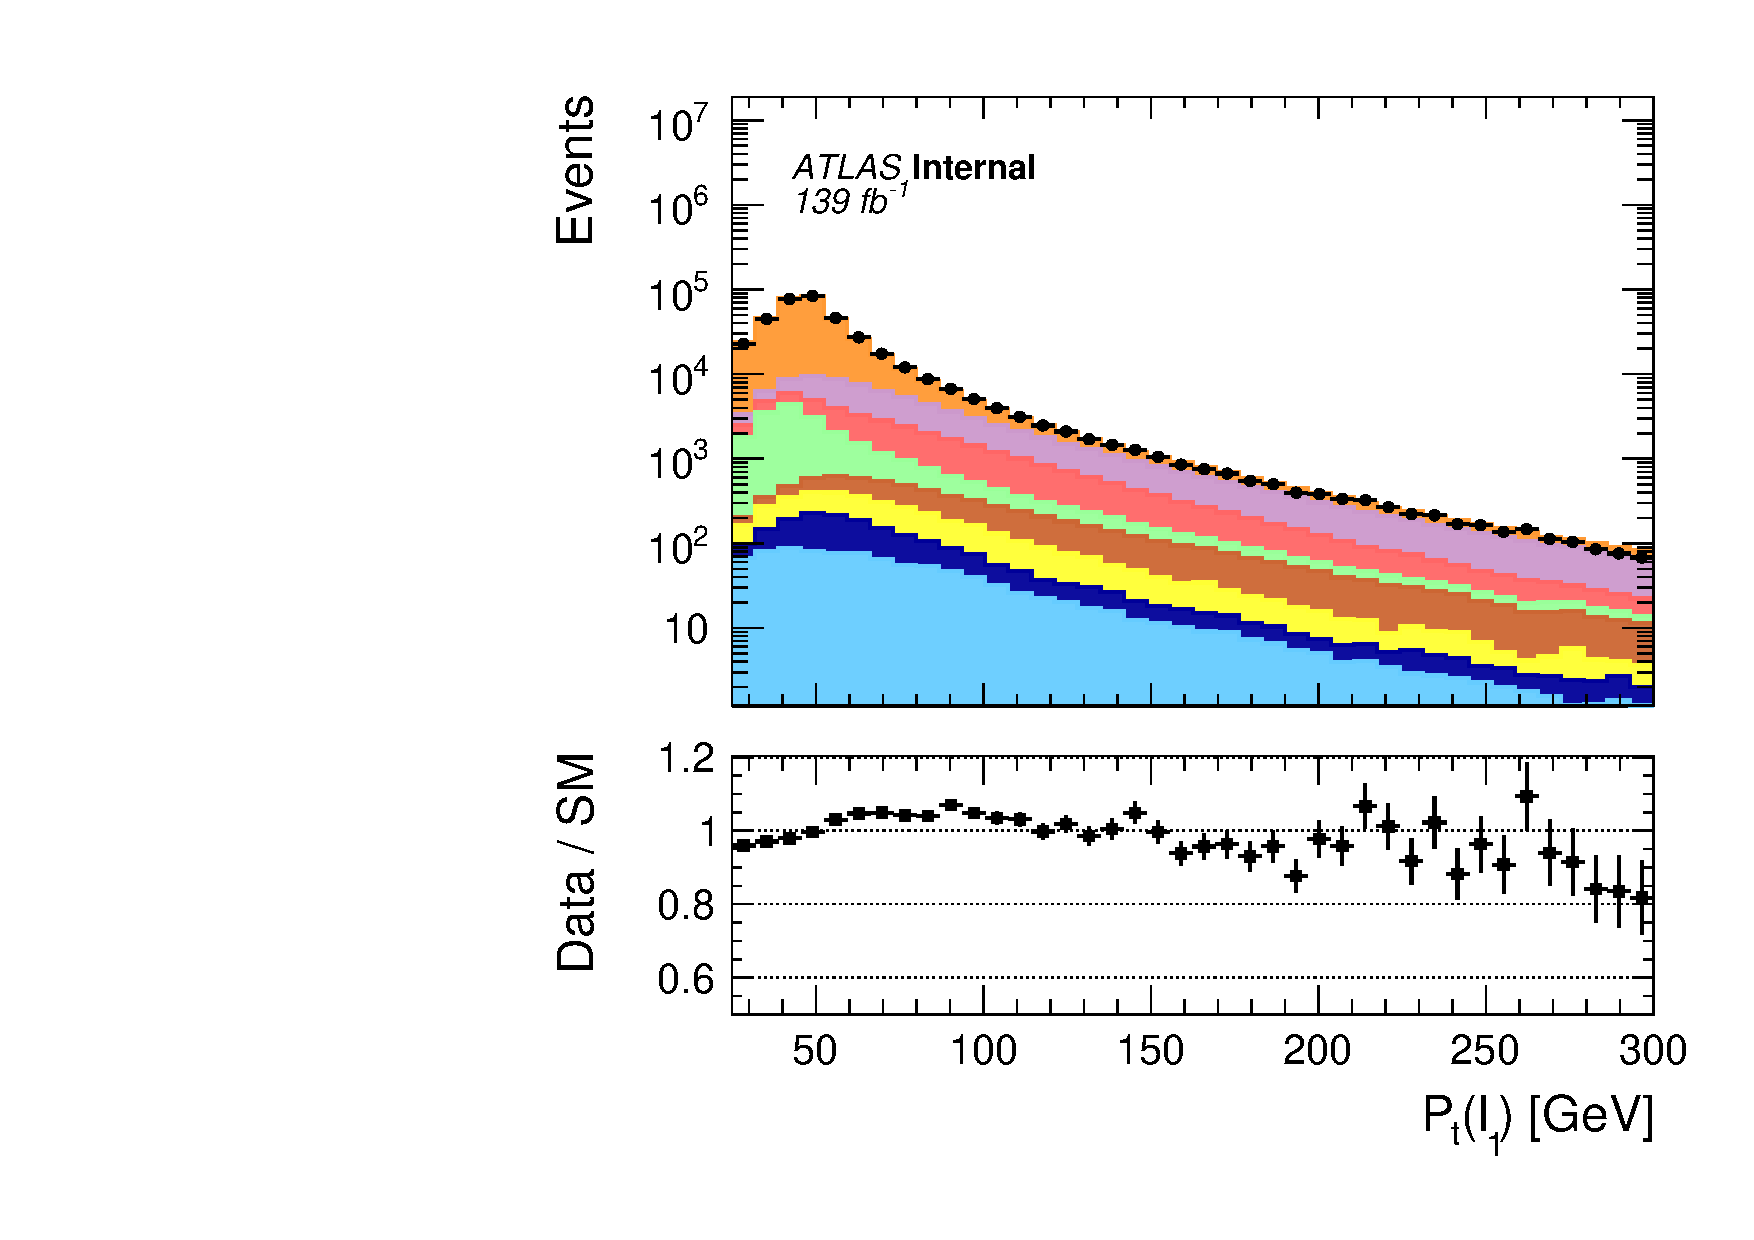
\includegraphics[width=\textwidth]{Figures/FeaturesHistograms/MCvsData/lep1_Pt.pdf}
        \caption{}
        \label{fig:lep1_Pt}
    \end{subfigure}
    \hfill
    \begin{subfigure}{.525\textwidth}
        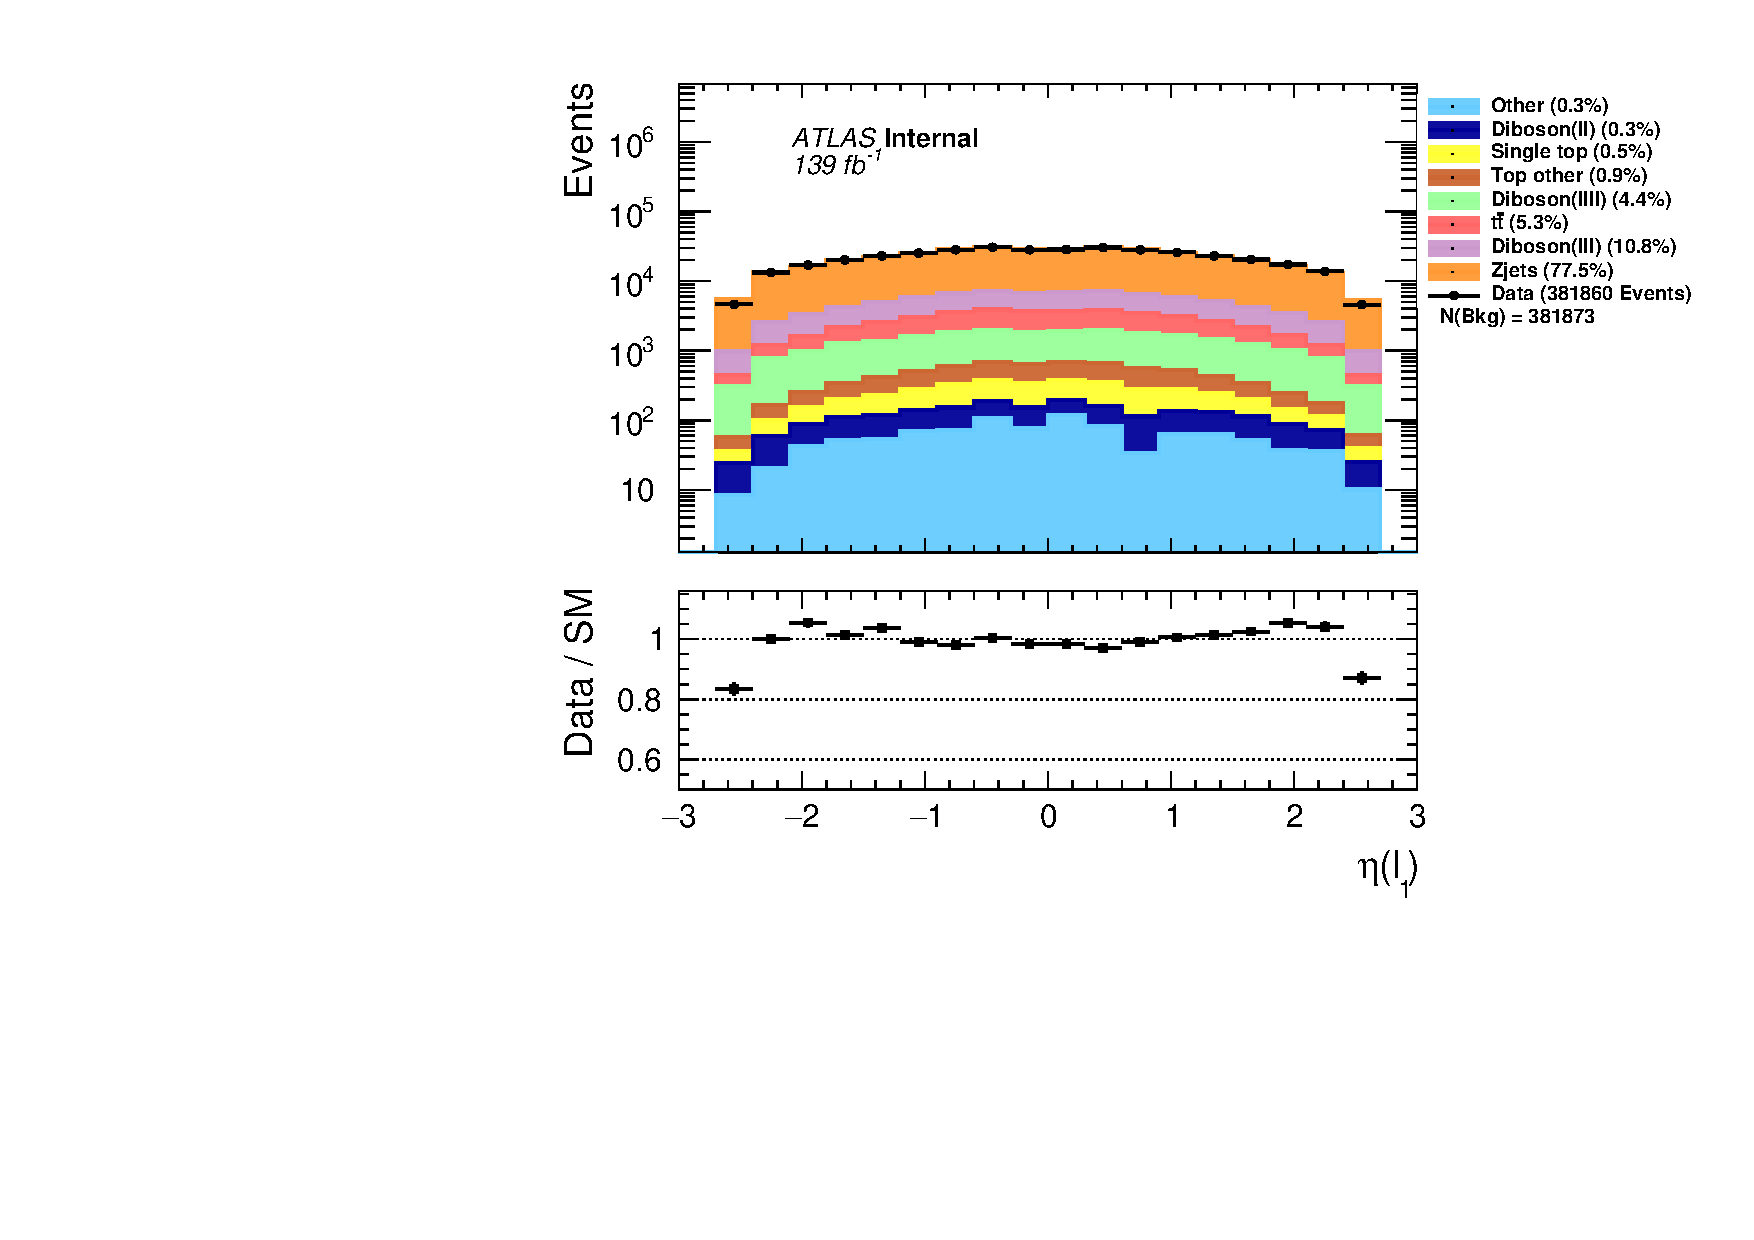
\includegraphics[width=\textwidth]{Figures/FeaturesHistograms/MCvsData/lep1_Eta.pdf}
        \caption{}
        \label{fig:lep1_Eta}
    \end{subfigure}
    }
    \makebox[0.95\linewidth][c]{%
    \begin{subfigure}{.405\textwidth}
        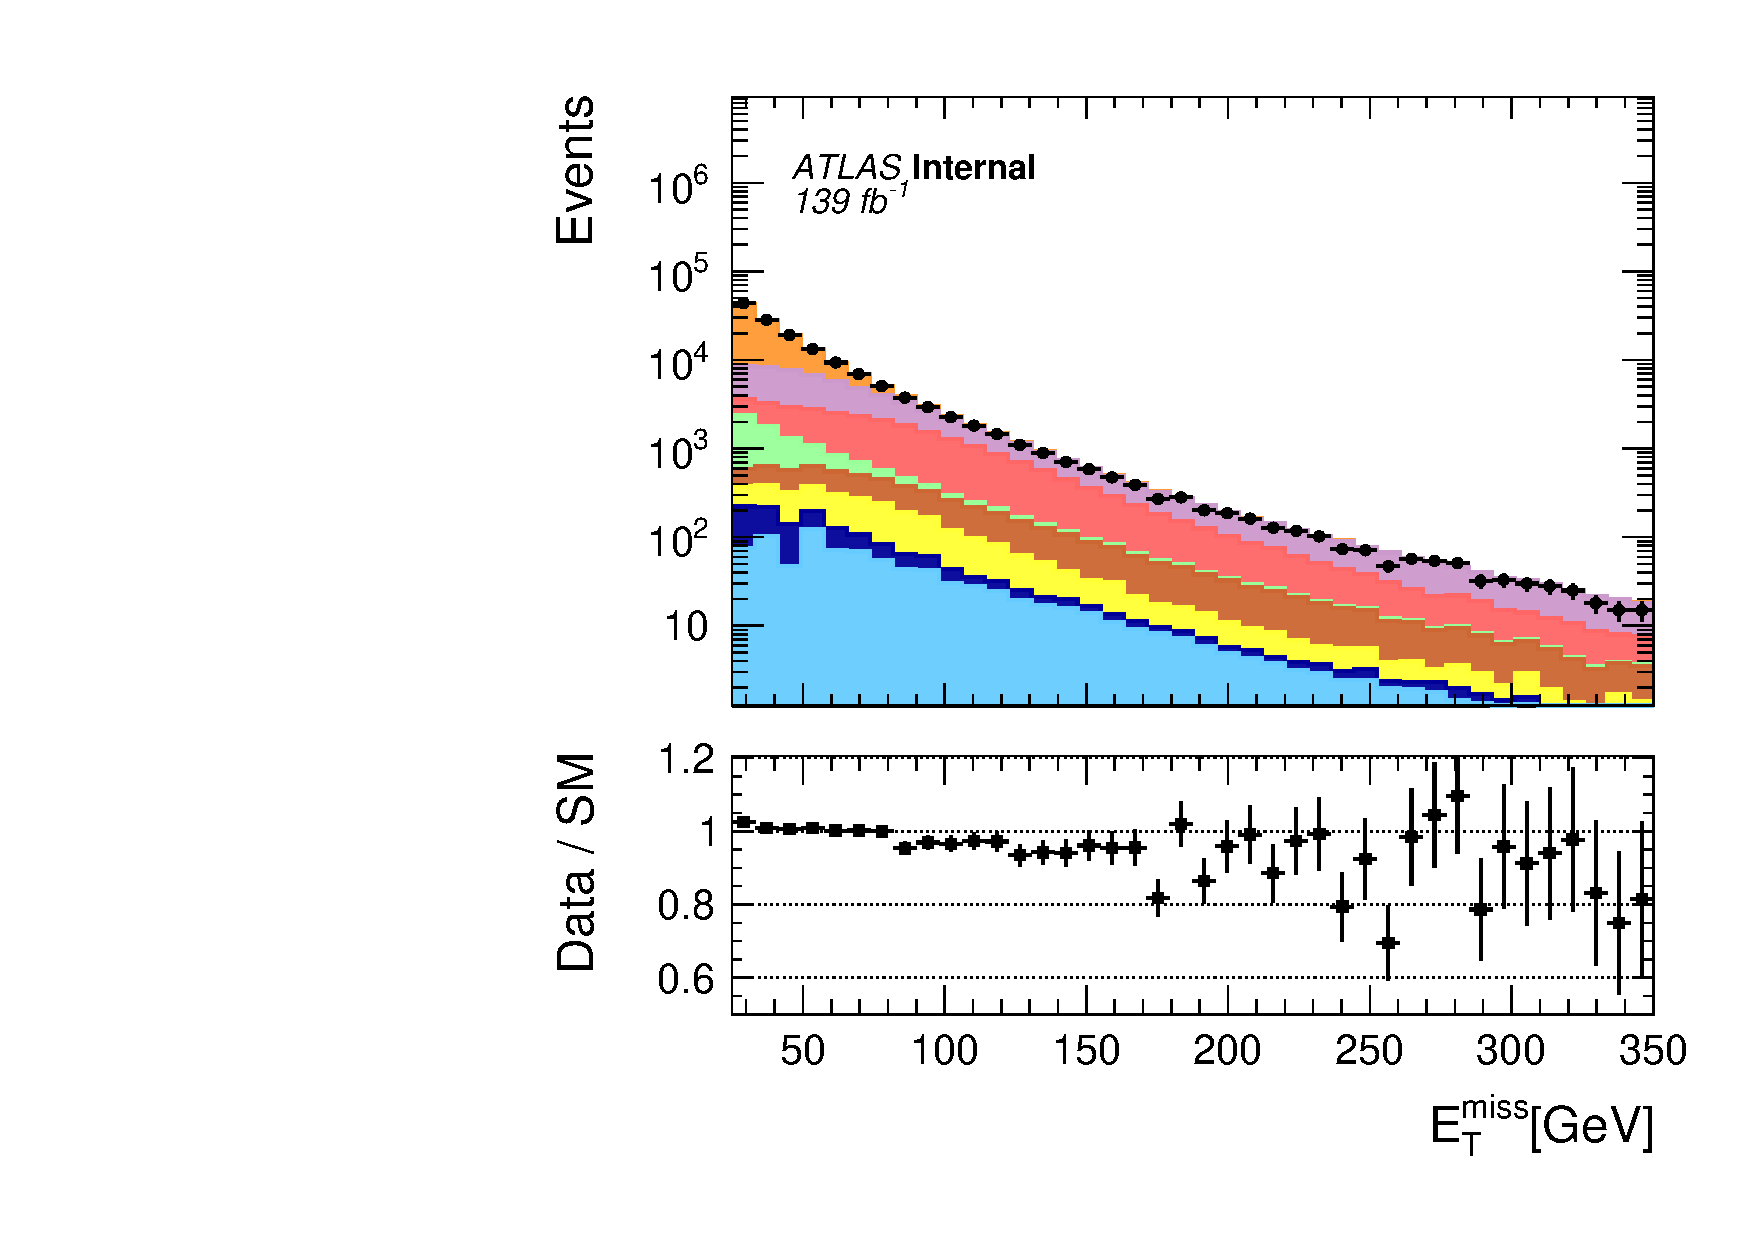
\includegraphics[width=\textwidth]{Figures/FeaturesHistograms/MCvsData/met_Et.pdf}
        \caption{}
        \label{fig:met_Et}
    \end{subfigure}
    \hfill
    \begin{subfigure}{.525\textwidth}
        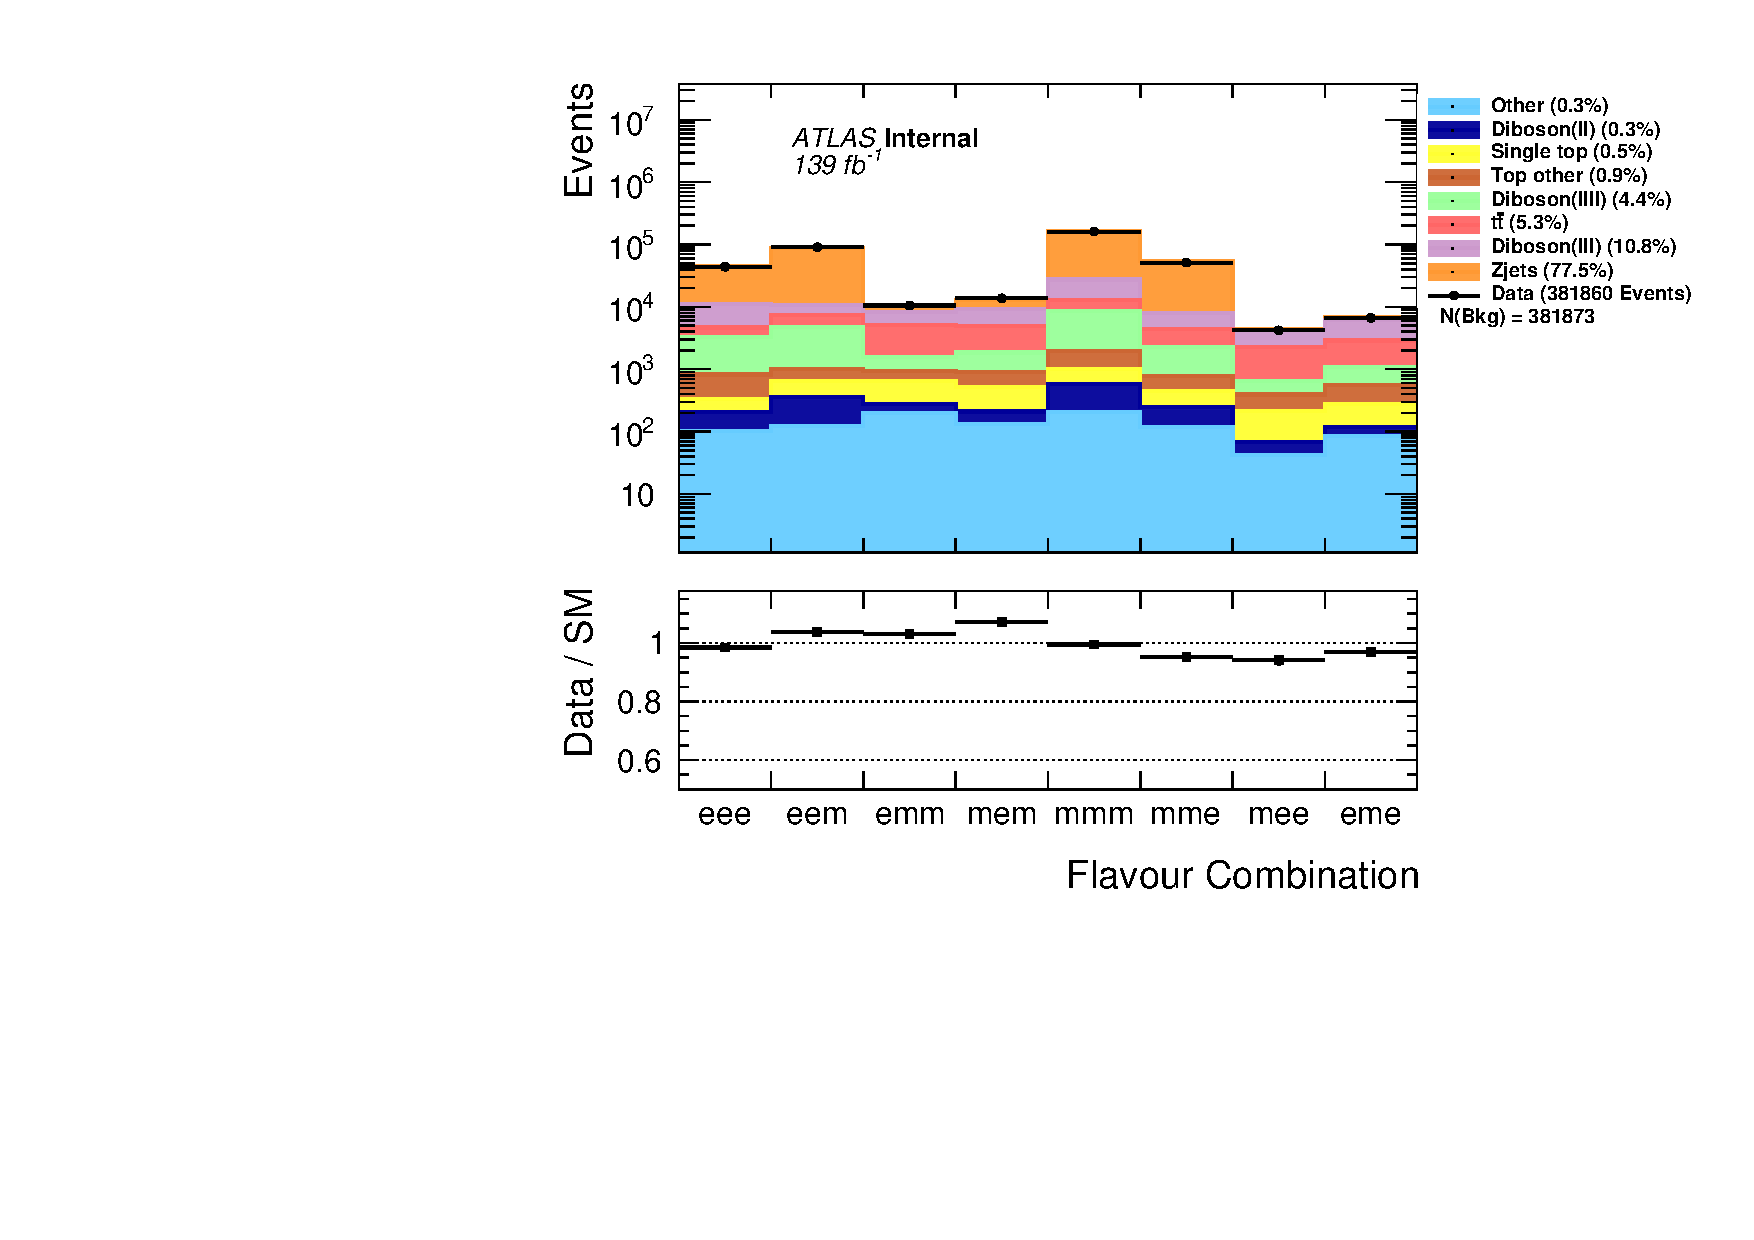
\includegraphics[width=\textwidth]{Figures/FeaturesHistograms/MCvsData/flcomp.pdf}
        \caption{}
        \label{fig:flcomp}
    \end{subfigure}
    }
    \caption{\ac{MC} and real data comparison and event distribution for each channel over $P_t$ \ref{fig:lep1_Pt} and 
    $\eta$ \ref{fig:lep1_Eta} for the first lepton. Similarly, the distribution over the $E_T^{miss}$ \ref{fig:met_Et}
    and flavor combination of the three leptons \ref{fig:flcomp}.}
    \label{fig:Dist1}
\end{figure}
\section{Handling Negative Weights in a BDT}\label{subsec:negWeights}
In section \ref{subsec:TraVal} I mentioned the inclusion of event-specific sample weights in the training 
of the \ac{ML} models. Most weights are in the range of $w_i \in [0,1]$, but some sample weights are negative.
The negative weight problem is a well known problem in the world of \ac{ML}-analysis for \ac{HEP}, 
and is a consequence of higher perturbative accuracy. For the purpose of visualizing 
distributions and training a \ac{NN}, negative weights are not a problem. But, when using 
the weights in the training of the \verb!XGBoost! classifier, the algorithm does not work\footnote{Upon further research 
in the codebase of XGBoost, it seems as though negative weights are not allowed as it interfere with XGBoost's use 
of the Hessian matrix. Due to time constraints, I decided not to  pursue this further.}.  
\\
Before deciding how to address the issue I decided to plot the distribution for 
a small subset of features for all the events with negative weights.
In figure \ref{fig:lep1_Pt_Neg} and \ref{fig:lep1_Phi_Neg} I plotted the distribution of the leading 
lepton for the features $p_T$ and $\phi$, but only including events with negative weights.
Additionally, I drew the distribution for the full data set for the same features in figures \ref{fig:lep1_Pt_nNeg}
and \ref{fig:lep1_Phi_nNeg}. By comparing the distributions, we can observe that the full data set and the 
negative weights' subset are very similar as well as only a fraction ($<10\%$) of the weights being negative.  
There are differences in distributions when comparing the \ac{SM} proccesess individually, but when studying the 
background as a whole, the two sets exhibit the same pattern across all regions. This means that the negative 
weights have little effect on the shape of the distribution of the full data set, which justifies choosing 
a simple solution to the issue. This, and the fact that the \ac{BDT} implementation is not of focus in the thesis, 
lead to the simplest solution to the problem being chosen.\\
\begin{figure}
    \makebox[0.95\linewidth][c]{%
    \centering
    \begin{subfigure}{.525\textwidth}
        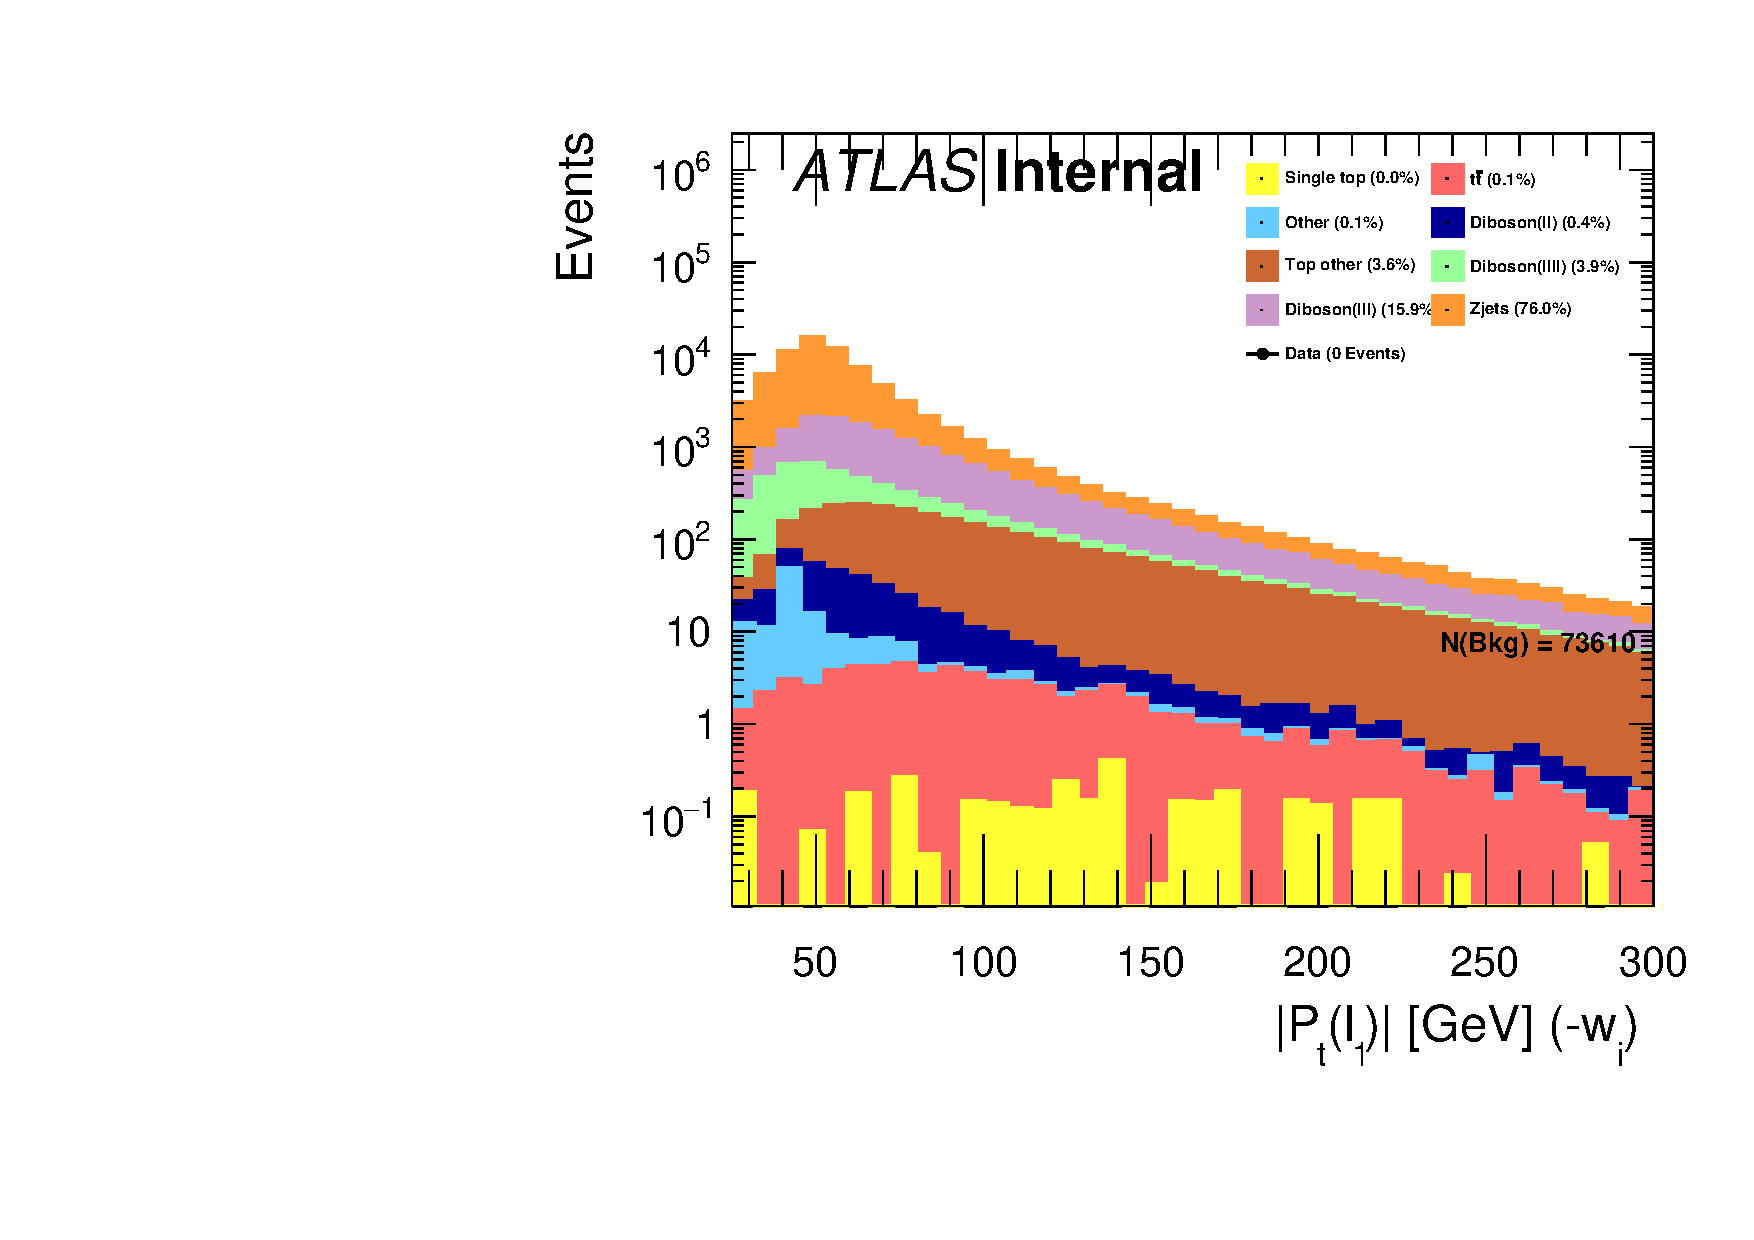
\includegraphics[width=\textwidth]{Figures/FeaturesHistograms/lep1_Pt_Neg.pdf}
        \vspace{-.75cm}
        \caption{}
        \label{fig:lep1_Pt_Neg}
    \end{subfigure}
    \begin{subfigure}{.525\textwidth}
        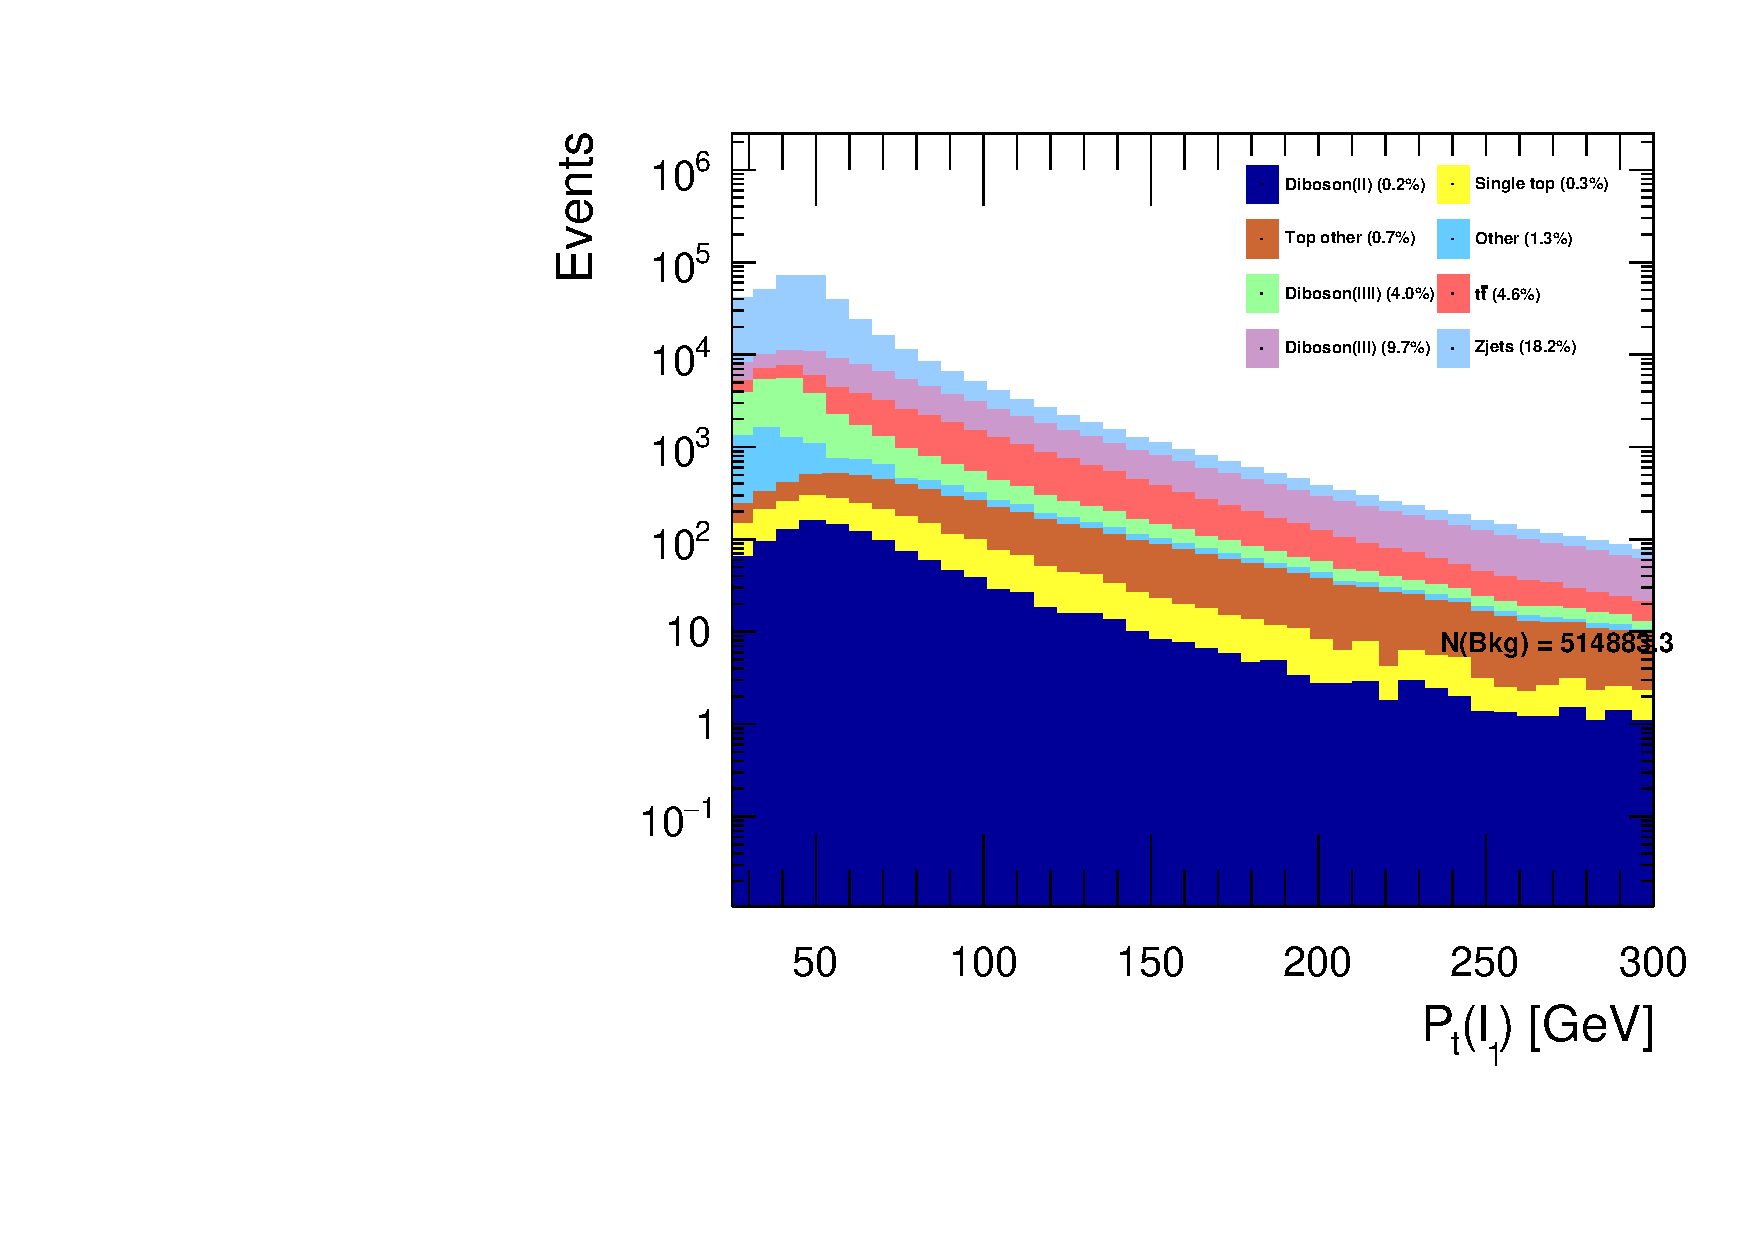
\includegraphics[width=\textwidth]{Figures/FeaturesHistograms/lep1_Pt_nNeg.pdf}
        \vspace{-.75cm}
        \caption{}
        \label{fig:lep1_Pt_nNeg}
    \end{subfigure}
    }
    \makebox[0.95\linewidth][c]{%
    \centering
    \begin{subfigure}{.525\textwidth}
        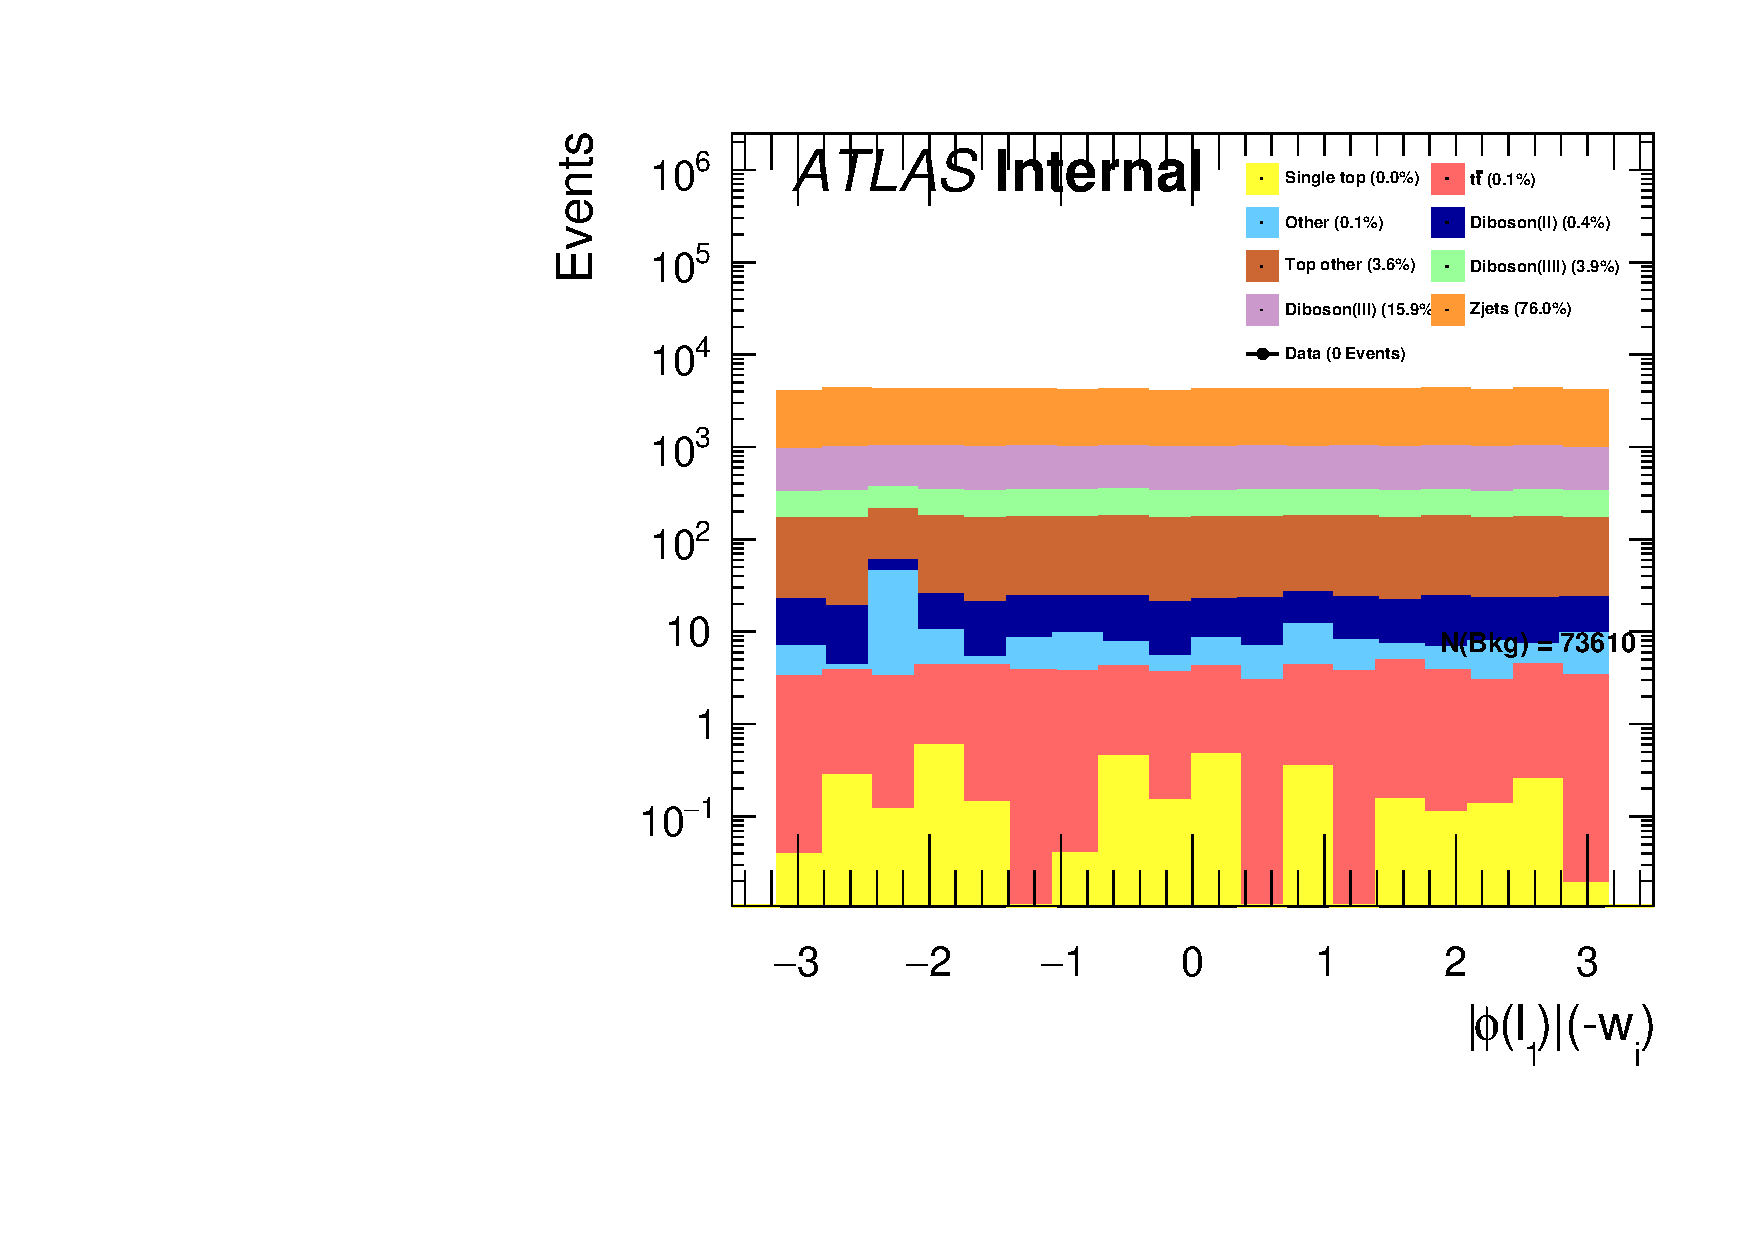
\includegraphics[width=\textwidth]{Figures/FeaturesHistograms/lep1_Phi_Neg.pdf}
        \vspace{-.75cm}
        \caption{}
        \label{fig:lep1_Phi_Neg}
    \end{subfigure}
    \begin{subfigure}{.525\textwidth}
        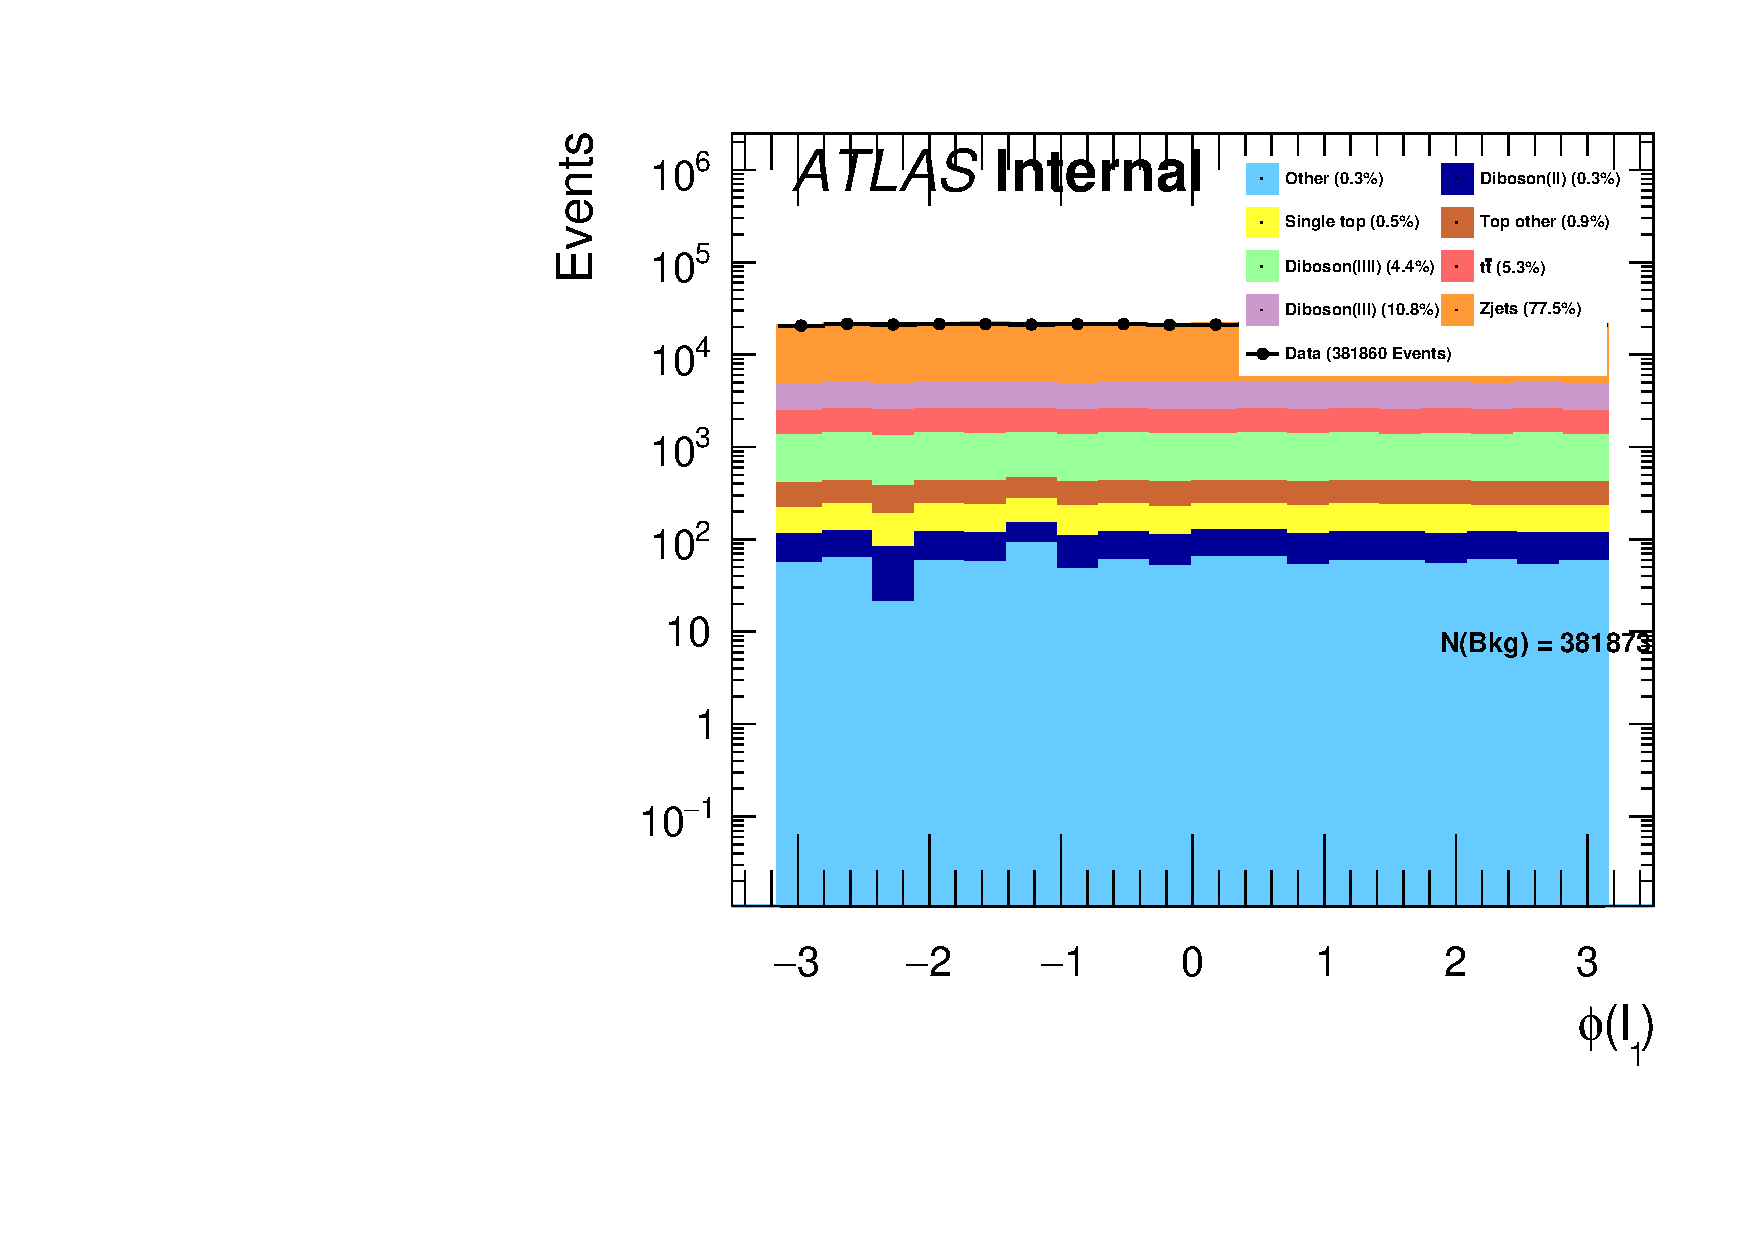
\includegraphics[width=\textwidth]{Figures/FeaturesHistograms/lep1_Phi_nNeg.pdf}
        \vspace{-.75cm}
        \caption{}
        \label{fig:lep1_Phi_nNeg}
    \end{subfigure}
    }
    \caption[The event distributions of the leading lepton for the features $P_t$ and $\phi$, for events with negative 
    weights and all events.]{The event distributions of the leading lepton for the features $P_t$ and $\phi$. 
    Figures \ref{fig:lep1_Pt_Neg} and \ref{fig:lep1_Phi_Neg} display only the events with 
    negative weights (for $P_t$ and $\phi$ respectively) whereas \ref{fig:lep1_Pt_nNeg} 
    and \ref{fig:lep1_Phi_nNeg} show the full data set.}
\end{figure}
The solution was inspired by the internal notes of the \ac{ATLAS} article \cite{Aad:2800889}, which introduced the solution 
when faced with the same problem. The solution is to take the absolute value and normalize all the weights, 
conserving the total sum of the weights and at the same time changing all negative signs. The simple procedure 
is shown bellow in equation \ref{eq:negw},
\begin{align}\label{eq:negw}
    w_i & = P \mid w_i \mid\,  \\
    P  & =  \sum_{j=0}^{N-1}\frac{ w_j}{\mid w_j \mid},
\end{align}
where $w_i$ is the weight of an event i, $i \in [0,N-1]$ and N equals the total number of events.
\section{Defining the Signal Region and Calculating the Significance}\label{sec:calcSign}
When producing an output I define the signal region through a brute force method which maximizes the significance. 
Based on trial and error and the study of the output from several models I found that, due to the unbalanced ratio of 
signal to background, a successful signal region would have to be very 'strict'. Therefore, for each model output I implemented a 
set of 200 cuts on the classifier output ranging from $0.9$ to the highest output of the model, with most cuts falling in the range of $>0.98$. For each cut
the significance is calculated where all signal and background events larger than said cut are included in the signal region. The cut 
corresponding to the largest significance is used to define the final signal region.  
\\
In most calculations of the significance I use equations \ref{eq:Z1}. This equation does not include any 
uncertainty, which is why any results using said equation is only for comparison reasons between the different \ac{ML}
models. In the final sections of the thesis I am interested in including an uncertainty to the results. To do this I utilize 
a function in \verb!ROOT!, the \texttt{RooStats.NumberCountingUtils.BinomialExpZ}\footnote{For more information on the function and the 
statistics behind it, see \url{https://root.cern/doc/master/rs__numbercountingutils_8C.html} (Accessed 08.05.2023).}, which takes the number of expected signal and background, 
as well as the systematic uncertainty of the background, and calculates a significance based on this.
\section{The Machine Learning Models}
\subsection{Model selection}
In this analysis I have chosen to compare 4 different "types" of \ac{ML}-models, ordinary dense \acf{NN}, \acf{PNN},
ensemble and \acf{BDT}. The first three methods are all types of \ac{NN}. I have deliberately 
chosen to focus on \ac{NN} given that there is far more freedom in the design of the architecture
of a \ac{NN}, than compared to a XGboost. Additionally, this was motivated by the selfish reason
being that I found the networks more interesting to study and dissect. Therefore, most of the 
analysis, comparisons and discussion is focused on the networks, while XGBoost is included 
as a loose benchmark. 
\\
The choice of the three network architectures is motivated in wanting to compare a simple 
deep network, a network ensemble and a \ac{PNN}. I would assume that the optimal architecture
would be a network which combines elements from each, but for the purpose of discussion
and research I have chosen to keep them somewhat separate. 
\subsection{Creating custom layers}\label{subsec:CustomLayer}
The field of \ac{ML} is one of the most dynamic and fastest growing fields of research
today. This means, that regardless of the brave attempt made by voluntary contributors and
the people at Google\footnote{The developers of TensorFlow}, there will always be 
new and exciting \ac{ML} tools and algorithm, not yet implemented in their library. This was 
certainly the case in this thesis. For several of the non-dense layers I was forced
to dive into the world of \ac{ML} development and create my own implementation. 
\\
All ensemble methods described in section \ref{subsec:LWTA} (except for dropout), channel-out, 
\ac{SCO} and maxout, resemble a layer already implemented by Tensorflow. This layer is called MaxPooling1D
\footnote{For more information on MaxPoolind1D, the reader is referred to the documentation 
($\href{https://www.tensorflow.org/api_docs/python/tf/keras/layers/MaxPool1D}{https://www.tensorflow.org/api_docs/python/tf/keras/layers/MaxPool1D}$,
accessed 24.03.2023).}. But, to allow for experimentation I decided to not use MaxPooling1D, but instead 
implement my own custom layers. All custom layers were implemented by creating new functions inside 
TensorFlow's dense layer, which are called when the network makes a prediction. In the following sections 
I will describe the algorithms underlying the implementation of each layer.
\subsubsection*{Channel-out}
In algorithm \ref{alg:channel-out} I summarized the implementation of channel-out used in this analysis. For each 
input which is to be passed through a forward-pass, the function first passes it through the weights and biases 
as described in section \ref{subsec:FP}. This is true for all the other layers as well. In line 7 I reshape the input 
to add a dimension which creates the units. In line 10 I create a new variable, $Output$ by reducing each unit to the 
largest activated node. Further I set each node to 0 which is not equal to the largest activation. Finally, I reshape 
the output to the original shape and return the output.  
\begin{algorithm}
    \caption{The pseudocode for implementing the channel-out layer in TensorFlow}\label{alg:channel-out}
    \begin{algorithmic}[1]
    \State def \textbf{Channel-out}(Input): 
    \State \ \ \ \ $\%$ Pass input through weight kernel and adding bias terms.
    \State \ \ \ \ $Input \gets Input \times Weights$
    \State \ \ \ \ $Input \gets Input + Bias$
    \\
    \State \ \ \ \ $\%$ Reshape input into units
    \State \ \ \ \ $Input \gets \textbf{Reshape}(Input,(Nr\ Units,\ Size \ of \ Units))$
    \\
    \State \ \ \ \ $\%$ Reduce input to the largest activation in each unit.
    \State \ \ \ \ $Output \gets \textbf{Max}(Input)$
    \\
    \State \ \ \ \ $\%$ Set original activation where activation is largest and 0 where it's not.
    \State \ \ \ \ $Output \gets \textbf{Where}(Input == Output, Input,0)$
    \\
    \State \ \ \ \ $\%$ Reshape to original size.
    \State \ \ \ \ $Output \gets \textbf{Reshape}(Output,(Input's \ Original \ Shape))$
    \State \ \ \ \ $\textbf{return}\ Output$
    \end{algorithmic}
\end{algorithm}
\subsubsection*{SCO}
In section \ref{subsubsec:stochchannelout} I described how \ac{SCO} is an extension of channel-out. This is certainly
also the case for the algorithms explaining the implementation. In algorithm \ref{alg:SCO} I have described 
algorithm used in the implementation of \ac{SCO} in this analysis. Similar to channel-out, the algorithm begins by 
passing input through weights and biases. Then, contrary to channel-out the nodes of the input are shuffled. This 
is to ensure that when the input is reshaped (in line 10), the units are made differently for each pass through 
the function. Again the maximum activation is found to create a new variable, this time called $OutputShuffle$. 
In line 16 $InputShuflle$ and $OutputShuffle$ are compared such that where $InputShuflle$ is equal to the largest 
activation, the value is set to 1 and otherwise set to 0. $OutputShuffle$ is then unshuffled, and reshaped to the 
original shape. Finally, the input which has been passed through the weights and biases, is multiplied with 
$Output$ and returned.
\begin{algorithm}
    \caption{The pseudocode for implementing the SCO layer in TensorFlow}\label{alg:SCO}
    \begin{algorithmic}[1]
    \State def \textbf{SCO}(Input): 
    \State \ \ \ \ $\%$ Pass input through weight kernel and adding bias terms.
    \State \ \ \ \ $Input \gets Input \times Weights$
    \State \ \ \ \ $Input \gets Input + Bias$
    \\
    \State \ \ \ \ $\%$ Shuffle all the values
    \State \ \ \ \ $InputShuflle \gets \textbf{Shuffle}(Input)$
    \\
    \State \ \ \ \ $\%$ Reshape input into units
    \State \ \ \ \ $InputShuflle \gets \textbf{Reshape}(InputShuflle,(Nr\ Units,\ Size \ of \ Units))$
    \\
    \State \ \ \ \ $\%$ Reduce input to the largest activation in each unit.
    \State \ \ \ \ $OutputShuffle \gets \textbf{Max}(InputShuflle)$
    \\
    \State \ \ \ \ $\%$ Set 1 where activation is largest and 0 where not.
    \State \ \ \ \ $OutputShuffle \gets \textbf{Where}(InputShuflle == OutputShuffle, 1,0)$
    \\
    \State \ \ \ \ $\%$ Un-shuffle all the values
    \State \ \ \ \ $Output \gets \textbf{UnShuffle}(OutputShuffle)$
    \\
    \State \ \ \ \ $\%$ Reshape to original size.
    \State \ \ \ \ $Output \gets \textbf{Reshape}(Output,(Input's \ Original \ Shape))$
    \\
    \State \ \ \ \ $\%$ Multiply input with output to set all input that are not the largest, to zero.
    \State \ \ \ \ $NewOutput \gets Input \times Output$
    \\
    \State \ \ \ \ $\textbf{return}\ NewOutput$
    \end{algorithmic}
\end{algorithm}
\subsubsection*{Max-out}
In algorithm \ref{alg:maxout} I have summarized the algorithm behind the implementation of the maxout layer.
Off the three layers (channel-out, \ac{SCO} and maxout), maxout was the simplest to implement. After passing 
the input through the weights and biases and reshaped to form the units, the input is reduced to only include 
the largest activation in each layer. Finally, the output is reshaped to the original shape and returned.
\begin{algorithm}
    \caption{The pseudocode for implementing the maxout layer in TensorFlow}\label{alg:maxout}
    \begin{algorithmic}[1]
    \State def \textbf{MaxOut}(Input): 
    \State \ \ \ \ $\%$ Pass input through weight kernel and adding bias terms
    \State \ \ \ \ $Input \gets Input \times Weights$
    \State \ \ \ \ $Input \gets Input + Bias$
    \\
    \State \ \ \ \ $\%$ Reshape input into units
    \State \ \ \ \ $Input \gets \textbf{Reshape}(Input,(Nr\ Units,\ Size \ of \ Units))$
    \\
    \State \ \ \ \ $\%$ Reduce input to the largest activation in each unit
    \State \ \ \ \ $Output \gets \textbf{Max}(Input)$
    \\
    \State \ \ \ \ $\%$ Reshape to size equal the number of units.
    \State \ \ \ \ $Output \gets \textbf{Reshape}(Input,(Nr \ Units))$
    \State \ \ \ \ $\textbf{return}\ Input$
    \end{algorithmic}
\end{algorithm}
\subsection{Model Architecture}\label{subsec:arch}
When choosing a network architecture, there are several ways to proceed. One way is to apply a grid search.
A grid search is simply defining a grid of parameters to test, then running through all combinations and 
choosing the highest performer. With a sufficient amount of tests, a grid search should converge towards 
an optimal architecture. Grid search is very common and there exists a large range of very complex varieties \cite{GS}.
For my analysis I chose not to perform a grid search, for several reasons. The first being interpretability.
Understanding a \ac{NN} is already hard, allowing for complex and unique architectures would only add another layer
of mysticism. The second is the size of the data set. The larger the data set, the larger the amount of data 
would be needed to adequately perform tests for each combination of parameters. Not only is this time-consuming,
but trying to mediate this issue could lead to poor performance. The third and most important reason is that 
I wanted to experiment with the architectures. By manually tuning the parameters, I was able to achieve a far 
better understanding of the final architecture. 
\begin{figure}
    \makebox[0.9\linewidth][c]{%
    \centering
    \begin{subfigure}{1.1\textwidth}
        \centering
        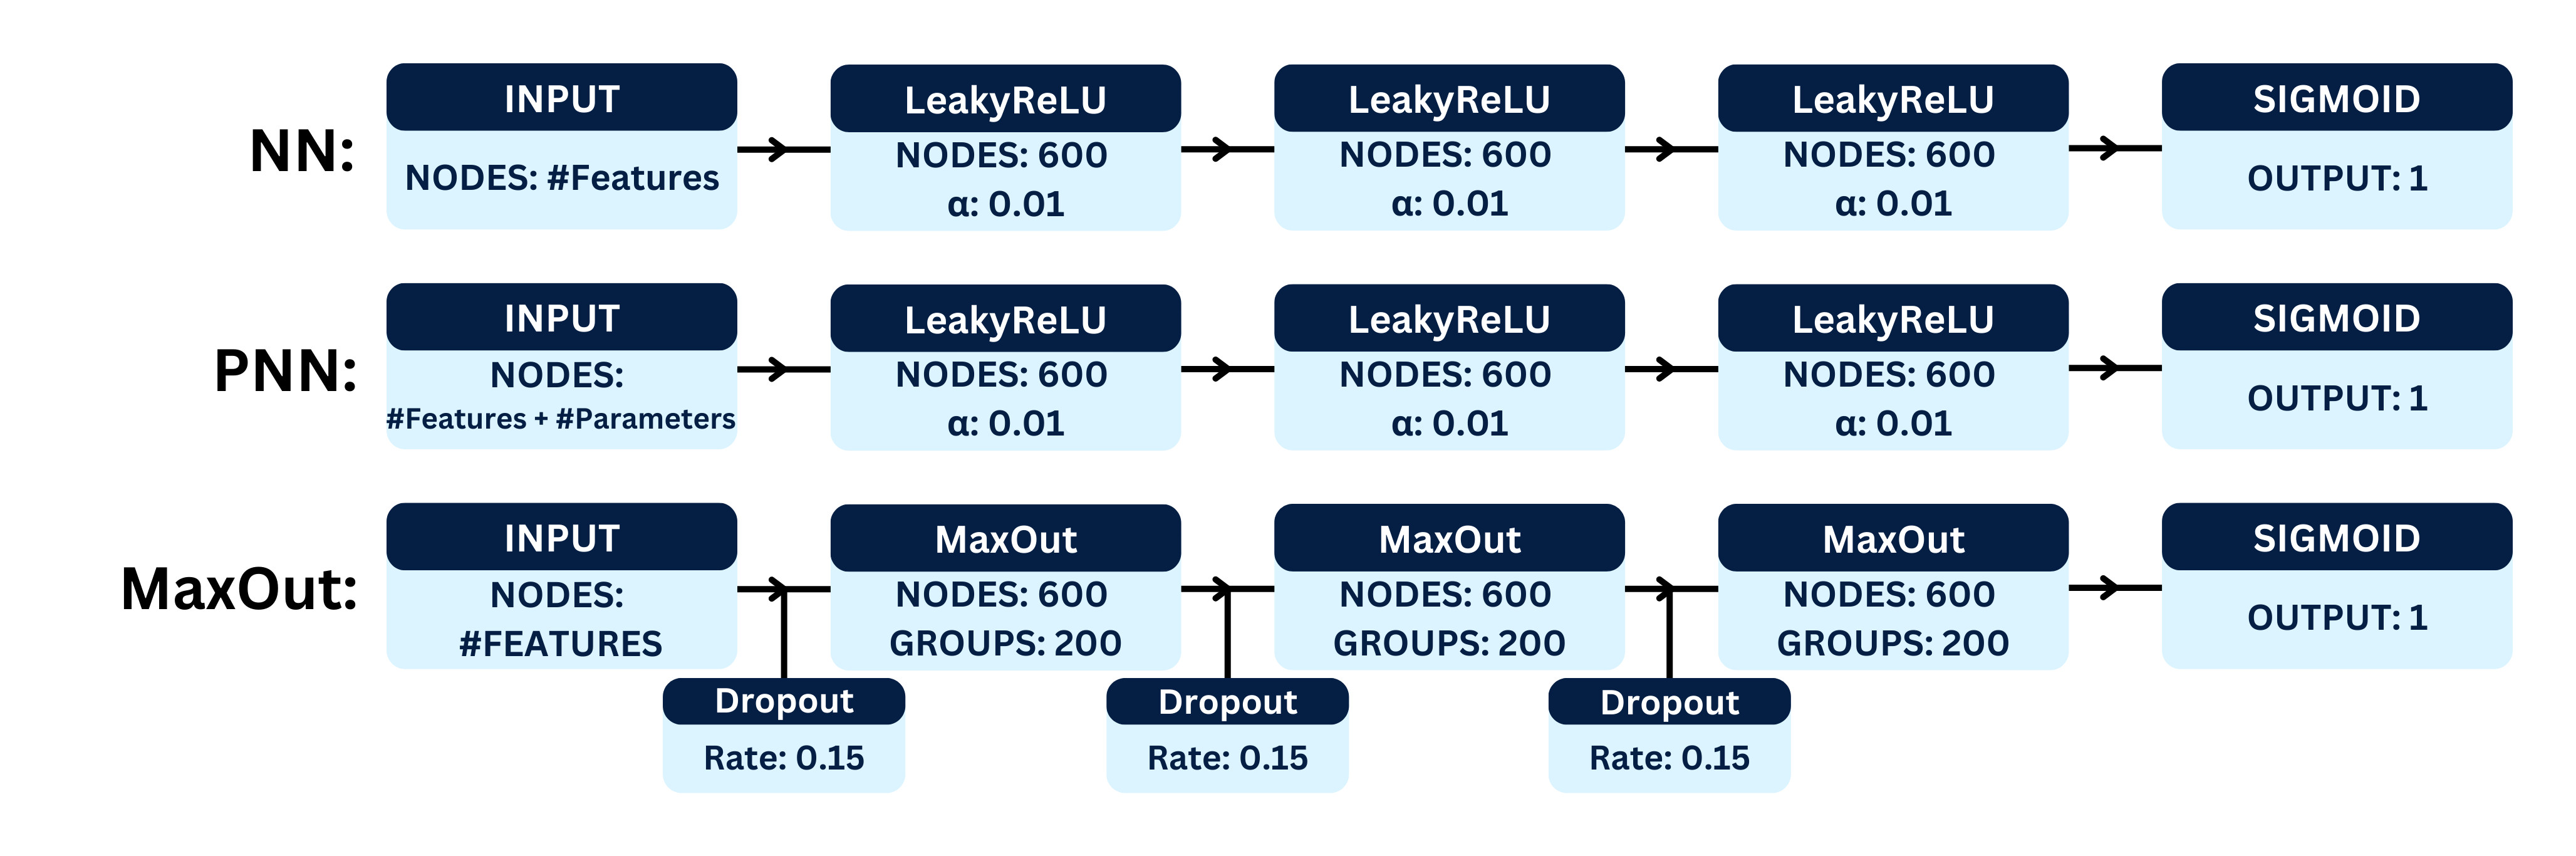
\includegraphics[width=\textwidth]{Figures/Illustrations/architecture.png}
    \end{subfigure}
    }
    \caption{A visual summary of the workflow and framework use for the 
    computational analysis. }
    \label{fig:arch}
\end{figure}
\subsection*{Dense Neural Network and PNN}\label{subsec:PNNArch}
The purpose of the simple dense \ac{NN}, is to compare the more complex networks to what is usually considered an ordinary dense \ac{NN}\footnote{Note 
that for the remaining part of this thesis, I will refer to this architecture as a 'dense \ac{NN}', 'ordinary dense \ac{NN}' and in some plots, just 
\ac{NN}}.
All layers are dense layers, meaning that all nodes in the previous layer are connected to the current layer, and likewise
the current layer is connected to the next. The general structure of the network is summarized in figure \ref{fig:arch}, with 
the network label \ac{NN}. The figure shows a dense \ac{NN} with 
three hidden layers, all with 600 nodes each. All hidden layers utilize the $LeakyReLU$ activation (see section \ref{subsec:activation})
with an $\alpha$ = 0.01. The architecture is designed to perform deep-training, and will train on a training set where all mass combinations 
are included\footnote{Contrary to training one network for each mass combination.}. 
\\
The \ac{PNN} architecture is like the name suggests, included to represent the model proposed by the article by Baldi et al. \cite{PNN}.
The architecture is illustrated in figure \ref{fig:arch}, with the label PNN. The figure shows a practically identical 
structure to the dense-\ac{NN}, with the only difference being in the input-layer. As was discussed in section \ref{subsec:PNN},
the \ac{PNN} includes the new physics signal free parameters\footnote{In our case, the masses of the \ac{BSM}-particles.} alongside the features
in the input layer.
\subsection*{MaxOut, Channel-Out and \ac{SCO}}
The ensemble methods are slightly more complex than both the dense \ac{NN} and \ac{PNN} in terms of architecture. To limit the complexity for comparison reasons
I choose to build an identical architecture for maxout, channel-Out and \ac{SCO}, with the only difference being which of the three layers is used.  
In figure \ref{fig:arch} I have illustrated the MaxOut architecture, with the label MaxOut. The figure shows a network with 6 hidden layers, 
3 MaxOut and 3 dropout. The network alternates between drop out and MaxOut, starting with dropout and finishing with MaxOut. The MaxOut layers 
have 600 nodes each which reduce down to the 200 nodes with the largest activation in their respective groups. Each dropout layer has a dropout 
rate of 0.15. Channel-out and \ac{SCO} have the same architecture to maxout, but replacing maxout with each of the two respectively. 

\subsection*{XGBoost}\label{subsec:XGBoost}
The main motivation to apply XGBoost is simply to benchmark my analysis, and therefore not a lot of effort has been put into the design of the 
architecture. As a consequence, the default parameters\footnote{See \href{https://xgboost.readthedocs.io/en/stable/parameter.html}
{https://xgboost.readthedocs.io/en/stable/parameter.html}
for a complete overview of default parameters.} of XGBoost have been used. The main parameters of the model are summarized as the following:
\begin{itemize}
    \item $\eta$ (learning-rate) = 0.3
    \item Max depth = 6
    \item Maximum number of trees = 100
\end{itemize}



\newpage
\section{Model Training and Validation}
\subsection{Training and Validating Data}\label{subsec:TraVal}
When building an \ac{ML}-model the usual approach is to divide your data into three sets; training, validation and 
testing. The training set is used to tune the internal parameters of the model, i.e. the weights and biases of a \ac{NN} or the cuts of a \ac{DT}.
The validation set is used to tune the hyperparameters of the model, for example the architecture of the \ac{NN} or the maximum depth of the \ac{DT}.
The test set should only be used when the model is finished, and is used to benchmark the model's performance. In our case, the performance we are 
interested in is the performance on the full \ac{MC}-background set and its comparison to the measured collision data. 
Therefore, in this analysis only two sets of data will be used, training and validation where both are sampled from the simulated
\ac{MC} data set. The validation set was added as a precaution to reduce overfitting when applied to the measured collision data.
\\
The overarching strategy in creating the training and validation set is summarized in the following steps:
\begin{enumerate}
    \item Shuffle the data set. 
    \item Split the data set in two, training ($80\%$) and validation ($20\%$)
    \item Scale the two data set such that the sum of the weights of the background is equal to the sum of the weights of the signal in each data set.
    \item Scale both data sets using the Standard Scalar approach (see section \ref{subsubsec:StandardScalar}) using the parameters (the mean and standard deviation) 
    of the training set on both sets.
\end{enumerate}
The first step ensures an equal distribution of processes in both data sets. The $80-20\%$ is a popular practice in \ac{ML} (see \cite{8020}) and was chosen 
here for convenience. The third step refers to the sample-weights introduced in section \ref{subsec:SGD}. The sample-weights are only included in the simulated data
(and therefore training data), to scale each simulated event based on the (among other things) probability of the collision, otherwise known as the cross-section. The scaling of the 
weights is done to ensure an equal prioritization for background classification and signal classification. In other words, if there was a large imbalance between signal and background, 
the model would be motivated to tune more towards one distribution in the feature space than another. The final step is motivated in the section regarding data handling \ref{subsubsec:StandardScalar}. 

\subsection{Training Strategy}\label{subsec:TrainingStrategy}
To best compare the different \ac{ML}-models, I decide to apply the same training strategy to all (including the \ac{BDT}). The strategy is simply to train the model 
with the training set, then apply an early-stopping algorithm (see section \ref{subsec:EarlyStopping}) with a cut-off based on the performance on the validation set. For 
every epoch the model makes a prediction on the validation data set, and logs the results. If more than 10 epochs go by without improving on the epoch with the best result,
training stops and the weights of the epoch corresponding to the best performance on the validation set are reset. This strategy was repeated for the \ac{BDT}, but logging 
for each new additional tree instead of epoch.
\\
The performance from each epoch was measured in \ac{AUC} (see section \ref{subsec:AUC}), where the \ac{AUC} was calculated with the same weighting as in training ($50\%$ signal
and $50\%$ background). The distribution of signal vs background is important when studying \ac{AUC}, as it will greatly affect the value. For example, a classifier which predicts 
both signal and background to be background is a poor classifier. But the larger the amount of background relative to signal, the higher the \ac{AUC} would be. 

%%%%%%%%%%%%% Results & Discussion %%%%%%%%%%%%%%
\chapter{Introduction to supervised and unsuperised machine learning}\label{chap:Intro ML}
Machine learning is rapidly becomming an overwhelming presens in many different scientific fields.
In areas ranging from cancer research to stock-trading, machine learning is being applied to probelms
once thought as impossible to solve. Particle physics, like many other fields is no exeption. Jet flavor classification \cite{Guest_2016}, 
separating jets from gluons \cite{PhysRevD.44.2025} or using \ac{ML} to create efficent \ac{SR} are just some examples
where \ac{ML} is a vital tool. The traditional approach for ML in high-energy physics is through the use 
of supperivsed learning. \ac{DNN}


\section{Dense Neural Networks}
\subsection{Deep vs Shallow}
\begin{figure}
    \makebox[\linewidth][c]{%
    \centering
    \begin{subfigure}{.65\textwidth}
        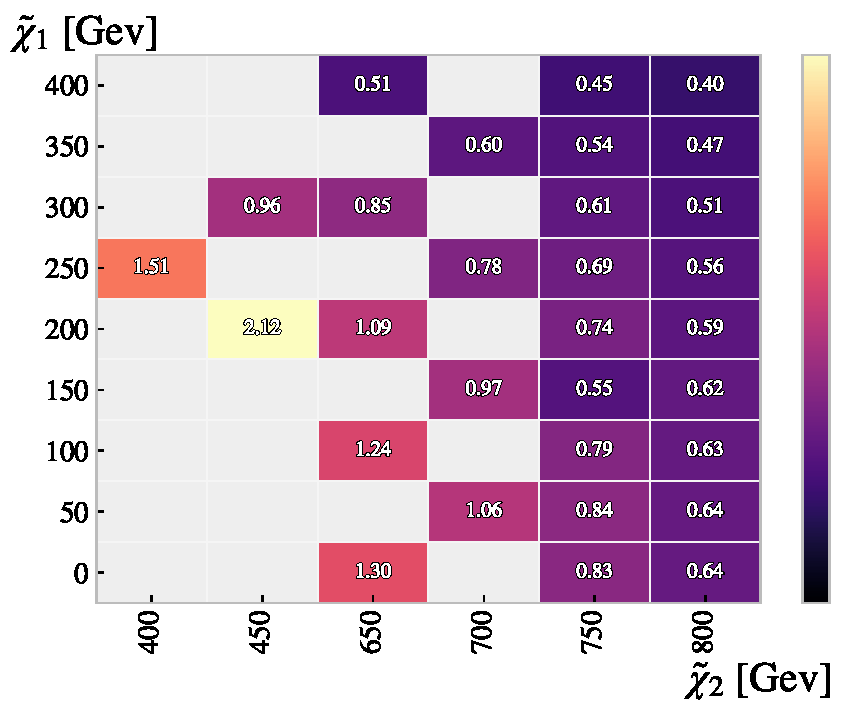
\includegraphics[width=\textwidth]{Figures/MLResults/NN/SUSY/Grid/NNshallowGridSig.pdf}
    \end{subfigure}
    }
    \caption{A grid displaying the achieved significance on the original signal set, using the signal region 
    created by the shallow \ac{NN}.}
    \label{fig:NNshallowGridSig}
\end{figure}
\begin{figure}
    \makebox[\linewidth][c]{%
    \centering
    \begin{subfigure}{.65\textwidth}
        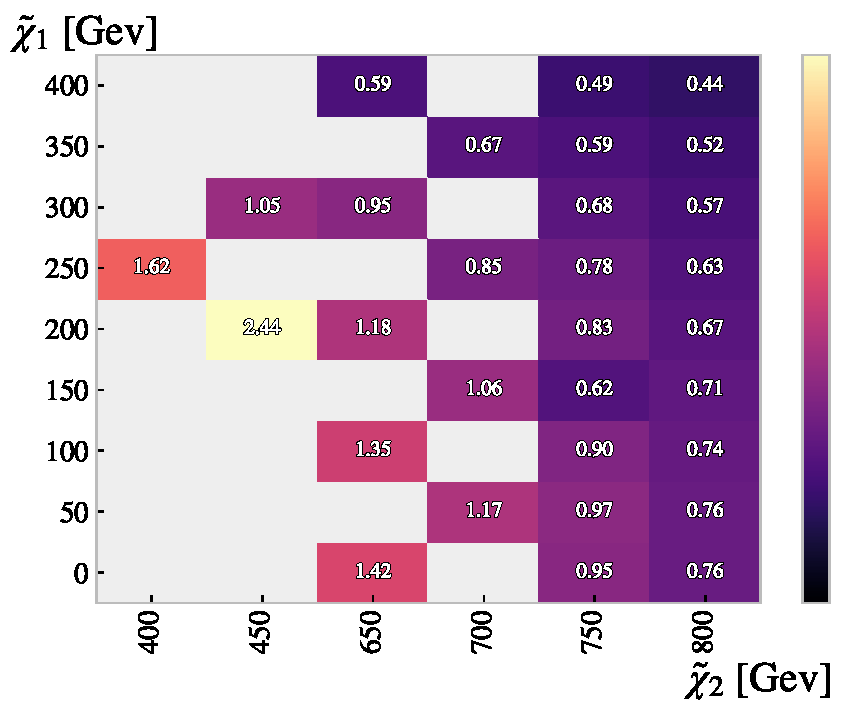
\includegraphics[width=\textwidth]{Figures/MLResults/NN/SUSY/Grid/NNGridSig.pdf}
    \end{subfigure}
    }
    \caption{A grid displaying the achieved significance on the original signal set, using the signal region 
    created by the dense \ac{NN}.}
    \label{fig:NNGridSig}
\end{figure}
\subsection{Parameter Specific Networks and Interpolation}
As I have touched upon in earlier sections, one possible solution to a diverse signal set (in my case a signal set with many 
potential mass combination) is to implement one model for each individual signal set. Initially one might assume that although 
this approach demands more work, it also produces the strongest performances for all mass combinations individually. I have already 
discussed how by including different mass combinations in the same signal, we hope to reduce overfitting and potentially allow 
the model to interpolate between the different mass combinations. However, I have not yet discussed how by moving from a one 
mass combination signal set to a diverse set would affect the performance on the original signal. In this section I will present the 
results from an analysis which aims to test the affirmation affect.
\\
In figure \ref{fig:Interpolation}, I present the results from two models who have each trained on two different amounts of signal.
The training used to produce the results aligns with the strategy described in section \ref{subsec:TrainingStrategy}.
Figure \ref{fig:OneMass} presents the achieved sensitivity from a dense \ac{NN} which has only trained on one mass combination,
($\tilde{\chi}_1=250$, $\tilde{\chi}_2=550$GeV), while figure \ref{fig:SeveralMass} presents the achieved sensitivity (using the same 
architecture) after training on a large set of mass combinations. Specifically, the latter figure shows the results after training on 
all signals on the outer square in the figure \ref{fig:SeveralMass} and ($\tilde{\chi}_1=250$, $\tilde{\chi}_2=550$GeV).\\
\begin{figure}
    \makebox[\linewidth][c]{%
    \centering
    \begin{subfigure}{.6\textwidth}
        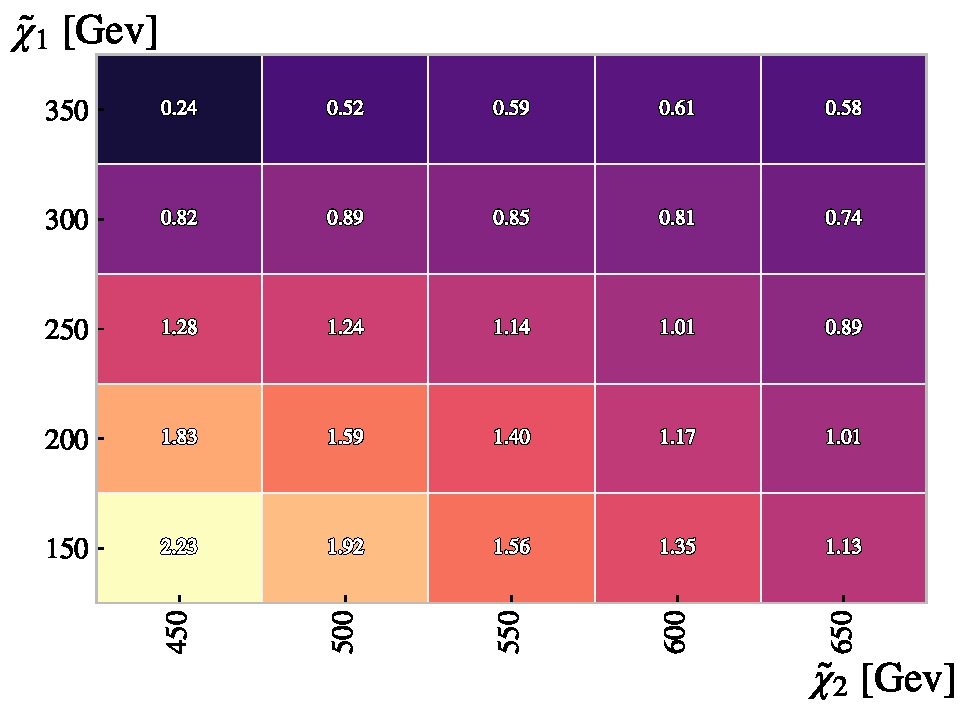
\includegraphics[width=\textwidth]{Figures/MLResults/NN/SUSY/Grid/Interpolation/NN_OneMass_InterpolationGridSig.pdf}
        \vspace{-1.cm}
        \caption{}
        \label{fig:OneMass}
    \end{subfigure}
    \hfill
    \begin{subfigure}{.6\textwidth}
        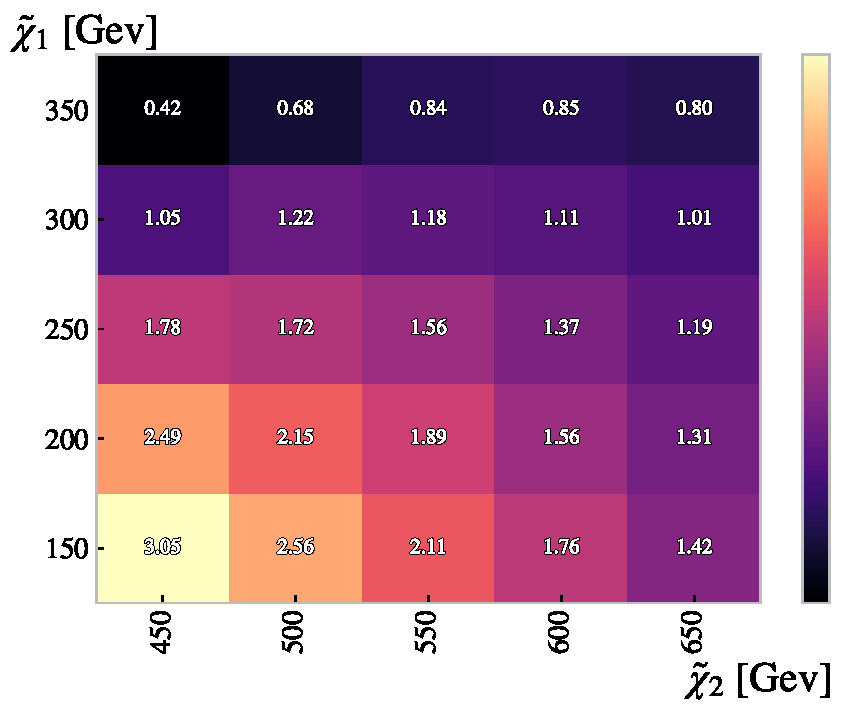
\includegraphics[width=\textwidth]{Figures/MLResults/NN/SUSY/Grid/Interpolation/NN_InterpolationGridSig.pdf}
        \vspace{-1.cm}
        \caption{}
        \label{fig:SeveralMass}
    \end{subfigure}
    }
    \caption{Two grids displaying the achieved significance on a subset of the full signal set, using the signal region 
    created by the \ac{NN}. Figure \ref{fig:OneMass} presents the results from a model who has only seen one mass combination 
    during training, ($\tilde{\chi}_1=250$, $\tilde{\chi}_2=550$GeV). Figure \ref{fig:SeveralMass} presents the results from 
    a model who has seen all mass combinations in the grid, but for the inner square of masses. }
    \label{fig:Interpolation}
\end{figure}
My initial prediction of this comparison, was that the one-mass model would outperform the several-masses model for the signal with
($\tilde{\chi}_1=250$, $\tilde{\chi}_2=550$GeV), while underperforming on all other data points. The expectation was that one-mass model 
would learn the trends of the only signal it had seen, while the several-masses model would do the same but for more mass combination and 
at the same time interpolate the results for the masses in between. By comparing figures \ref{fig:OneMass} and \ref{fig:SeveralMass} we 
see that my prediction was not completely true. We can observe that the model which has trained on several-masses outperformed the 
one-mass model on every single signal. At first, I believed this to be caused by the one-mass model overfitting a lot sooner than the other 
model, therefore being stopped earlier in training by the early-stopping criteria described in section \ref{subsec:TrainingStrategy}. 
To test this theory, I drew the training history of each training session.
\\
In figure \ref{fig:InterpolateHistory} I drew the \ac{AUC} score made after each epoch on both the training and validation set
for the one-mass model (\ref{fig:oneMassHist}) and the several-masses model \ref{fig:SeveralMassHist}. By comparing the two figures,
we observe that the one-mass models performance on the validation set peaks in the first epoch, therefore stopping training after 
10 epochs, while the several-masses model peaks after 6 epochs. This is a clear indication that training on one mass combination, leads 
to overfitting. 
\begin{figure}
    \makebox[\linewidth][c]{%
    \centering
    \begin{subfigure}{.45\textwidth}
        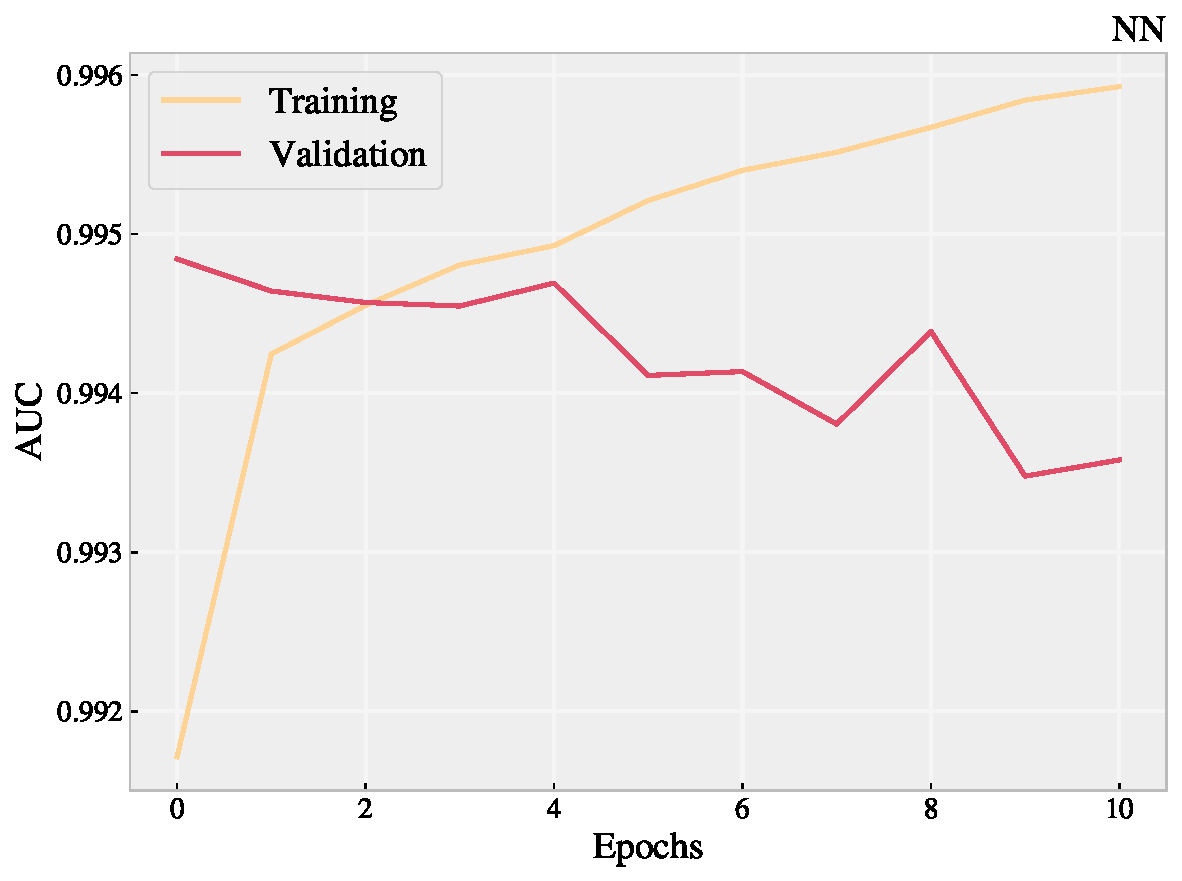
\includegraphics[width=\textwidth]{Figures/MLResults/NN/SUSY/History/NN_OneMass_InterpolationHistory.pdf}
        \caption{}
        \label{fig:oneMassHist}
    \end{subfigure}
    \begin{subfigure}{.45\textwidth}
        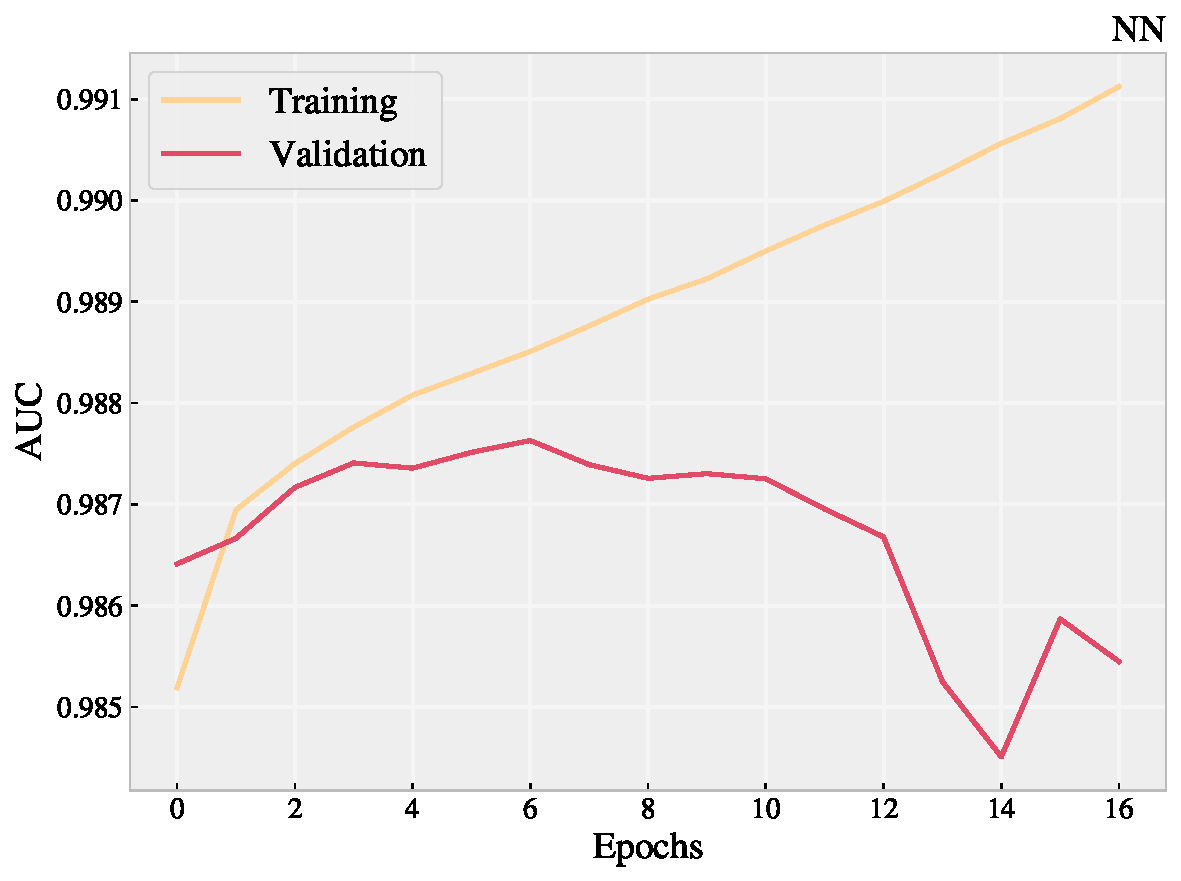
\includegraphics[width=\textwidth]{Figures/MLResults/NN/SUSY/History/NN_InterpolationHistory.pdf}
        \caption{}
        \label{fig:SeveralMassHist}
    \end{subfigure}
    }
    \caption{A plot displaying the \ac{AUC} score made after each epoch on both the training and validation set. 
    Figure \ref{fig:oneMassHist} shows the results from the one-mass model and figure \ref{fig:SeveralMassHist} shows
    the results from the several-masses model.}
    \label{fig:InterpolateHistory}
\end{figure}
\\
Given the one-mass models performance is reduced by the early-stopping criteria, I wanted to explore if it would be able to outperform the 
several-masses model given it was allowed to train deeper. In figure \ref{fig:NNOverfitting}, I display the achieved significance
of the one-mass model in the case where early-stopping has been removed, and the model was allowed to train for 15 epochs. By comparing figures 
\ref{fig:SeveralMass} and \ref{fig:NNOverfitting}, we can observe that even when early-stopping is removed from the one-mass model, it is  
still outperformed by the several-masses model. This indicates that overfitting is not the only reason for the one-mass models disappointing performance.\\
\begin{figure}
    \centering
    \makebox[\linewidth][c]{%
    \begin{subfigure}{.6\textwidth}
        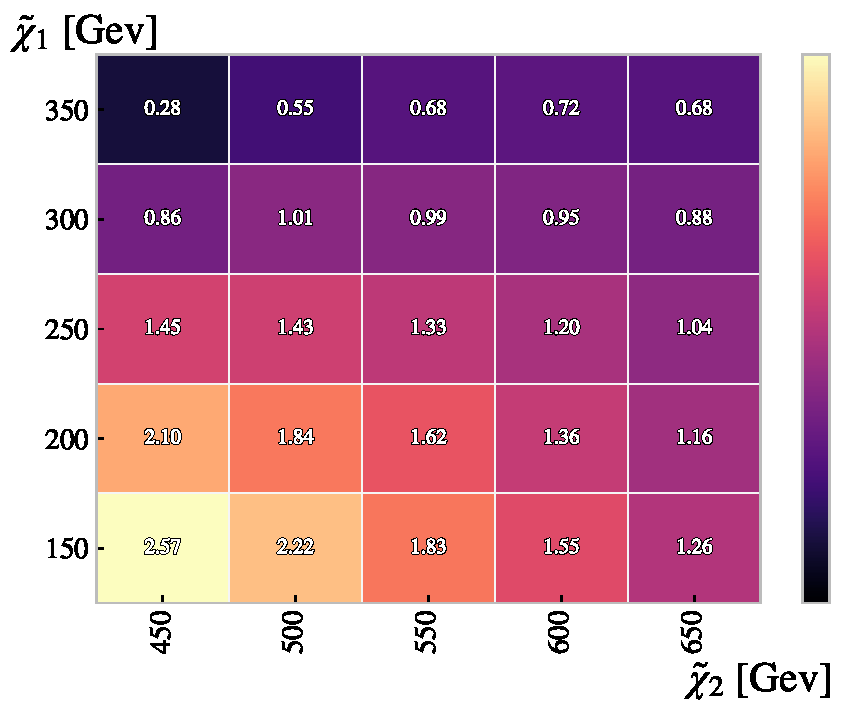
\includegraphics[width=\textwidth]{Figures/MLResults/NN/SUSY/Grid/Interpolation/NN_OneMass_Overfitting15_InterpolationGridSig.pdf}
    \end{subfigure}
    }
    \caption{A grid displaying the achieved significance on a subset of the full signal set, using the signal region 
    created by the \ac{NN}. The figure presents the results from a model who has only seen one mass combination 
    during training, ($\tilde{\chi}_1=250$, $\tilde{\chi}_2=550$GeV) and was allowed to train for 15 epochs without 
    early-stopping.}
    \label{fig:NNOverfitting}
\end{figure}
The most probable explanation for the underwhelming performance of the one-mass model, is that nearby mass combinations (i.e. mass combination with 
relatively similar masses) exhibit a lot of overlap in terms of feature trends. In other words, nearby mass combinations (in this example, mass combinations 
differ by 100GeV) often contribute to the same type of training. This means that by including a larger range of signals, which are similar in mass, we are 
essentially increasing the amount of data for each individual signal.
\section{Ensemble methods}\label{sec:Ensemble}
\subsection{Visualizing Sparse Pathways}\label{subsec:Viz}
As mentioned in section \ref{subsec:CustomLayer}, the channel-out, \ac{SCO} and maxout layers applied in this 
analysis were created by me using the \verb!TensorFlow! \ac{API}. As such, I found it imperative to make
sure that the layers worked as intended. To do this I created a small network with three layers, with eight 
nodes each, all applying maxout layers with four, two and four units respectively. In this section I will 
dissect the activations of said network before and after training.
\\
In figure \ref{fig:BTraining}, I have plotted the activation of 100 randomly sampled events, 50 
background and 50 signal for an untrained model. Adjacent, I plotted the resulting distribution of the 
output. From the figure we observe little to no difference between the activation from the signal and 
the background. This is mirrored in the distribution of the output which is centered around the middle 
of the range. This result is as expected, given that an untrained model holds no knowledge of the data and 
simply applies a random set of weights. A small exception from this result can be found for larger output values, 
where we observe a small distribution of signal values. This is due to the signal having some inherit differences
to the background (for example high $E_t^{miss}$).
\\
In figure \ref{fig:ATraining}, I plotted a similar plot as described above, but using a trained model.
In this figure the output is far more separated, and we see noticeable differences in the activation 
of nodes. To highlight the difference in activation, I drew two new figures where the signal 
(\ref{fig:ATrainingSig}) and background (\ref{fig:ATrainingBkg}) were drawn individually.
In figure \ref{fig:NetDist1} we notice that there is a noticeable variation in the activation for
both signal and background. The differences are highlighted in the different paths through network, indicating the
model is able to differentiate between signal and background. Most noticeably, the two units 
in the middle hidden layer highlight this fact. In the case of the signal, the upper unit clearly favors 
the second bottom node. For the background this is also partly true, but with far more 
spread in the other nodes. Similarly, in the bottom unit (in the same layer), the background shows large
activation in the uppermost node, while the signal data does not. To conclude, the maxout layer does indeed 
find specific paths through the network which will aid in separating the output for the signal and the background.\\
\begin{figure}
    \makebox[\linewidth][c]{%
    \centering
    \begin{subfigure}{.6\textwidth}
        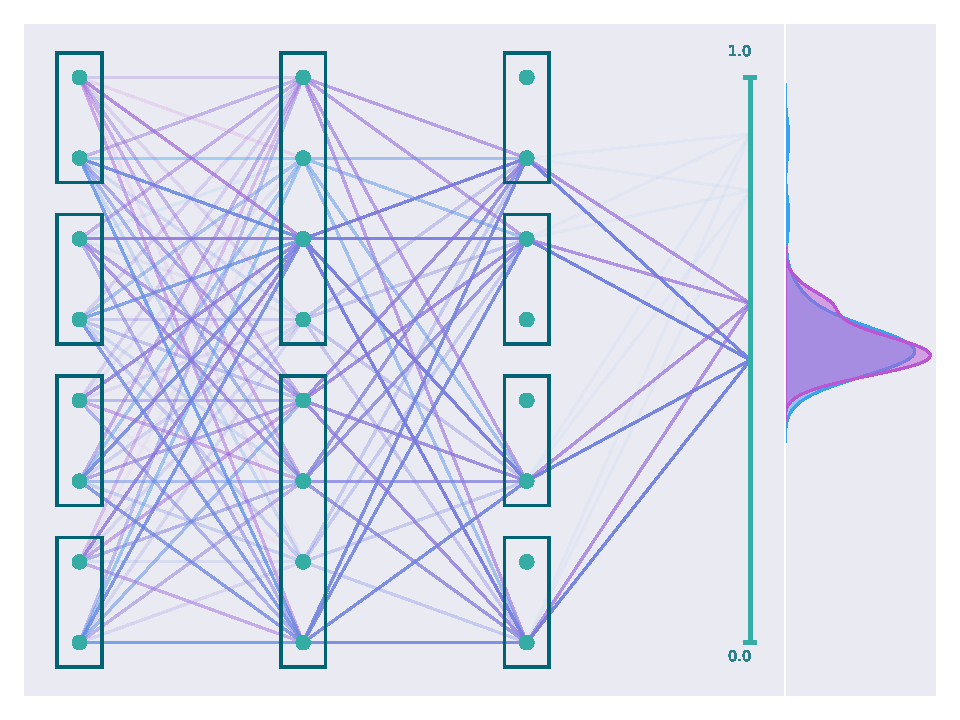
\includegraphics[width=\textwidth]{Figures/MLResults/NN/NetworkVis/BeforeTraining.pdf}
        \caption{}
        \label{fig:BTraining}
    \end{subfigure}
    \hfill
    \begin{subfigure}{.6\textwidth}
        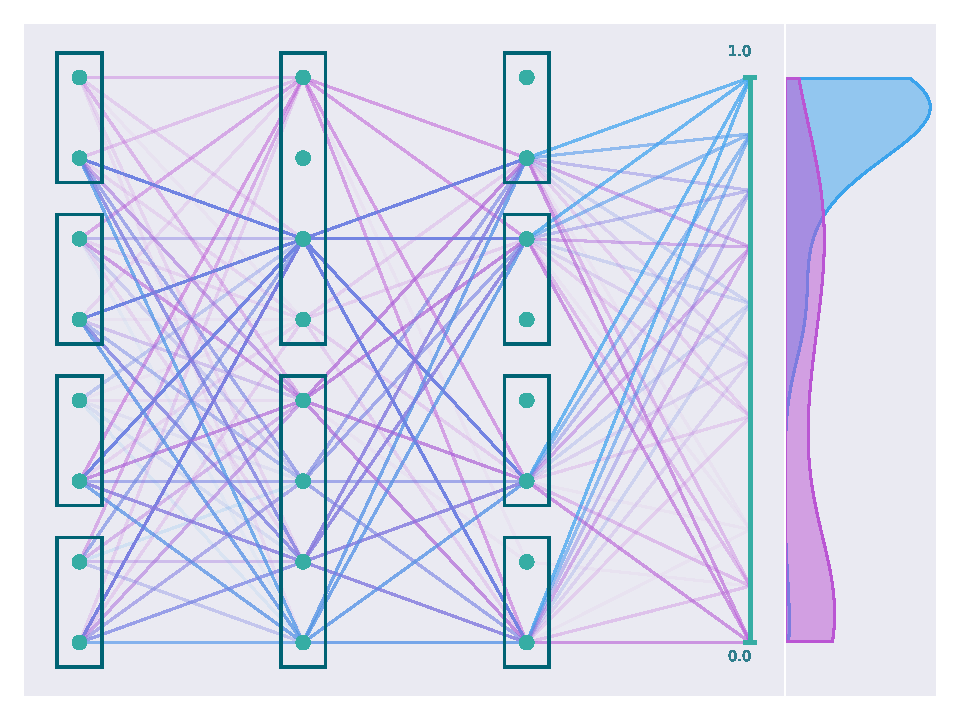
\includegraphics[width=\textwidth]{Figures/MLResults/NN/NetworkVis/AfterTraining.pdf}
        \caption{}
        \label{fig:ATraining}
    \end{subfigure}
    }
    \caption[A calculated visualization of the activation of a three layer maxout network, before and after training.]{
    A calculated visualization of a three layer maxout network. Each path 
    represents a data point where all connected nodes were the largest activation in their respective 
    unit. The distribution on the far right represent the output distribution. The figure to the left
    (\ref{fig:ATrainingSig}) is the result before training and the figure to right (\ref{fig:ATrainingBkg})
    is after.}
\end{figure}
\begin{figure}
    \makebox[\linewidth][c]{%
    \centering
    \begin{subfigure}{.6\textwidth}
        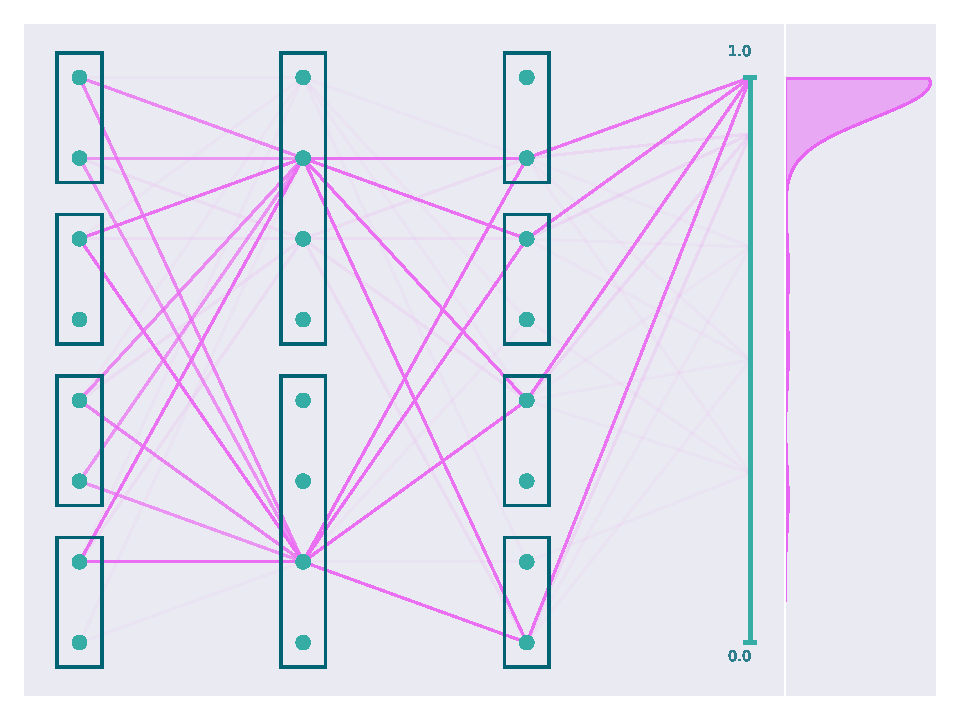
\includegraphics[width=\textwidth]{Figures/MLResults/NN/NetworkVis/AfterTrainingSig.pdf}
        \vspace{-0.5cm}
        \caption{}
        \label{fig:ATrainingSig}
    \end{subfigure}
    \hfill
    \begin{subfigure}{.6\textwidth}
        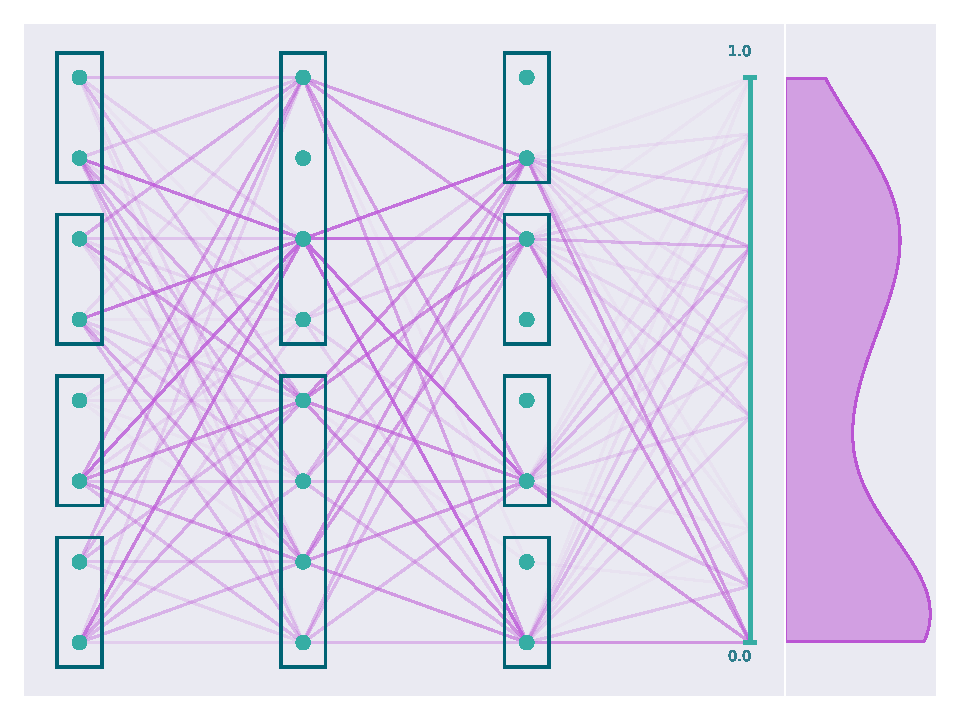
\includegraphics[width=\textwidth]{Figures/MLResults/NN/NetworkVis/AfterTrainingBkg.pdf}
        \vspace{-0.5cm}
        \caption{}
        \label{fig:ATrainingBkg}
    \end{subfigure}
    }
    \caption[A calculated visualization of the activation of a three layer maxout network, after training and displaying the
    signal and background separately.]{A calculated visualization of a three layer maxout network. The lines represent the path 
    through the nodes with the largest activation in their respective unit. The bolder the line the more frequently the path is 
    used. The distribution on the far right represent the output distribution and the figure with blue 
    paths (left) \ref{fig:ATrainingSig} is the result of signal, and the pink paths (right) is a result from background 
    \ref{fig:ATrainingBkg}.} 
    \label{fig:NetDist1}
\end{figure}

\begin{figure}
    \makebox[\linewidth][c]{%
    \centering
    \begin{subfigure}{.6\textwidth}
        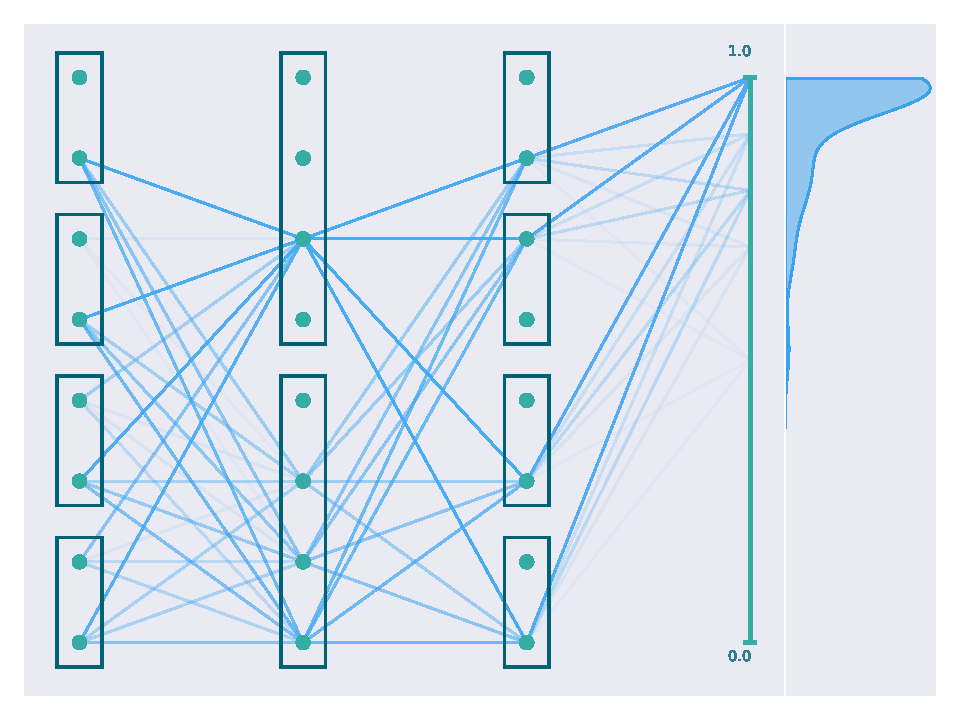
\includegraphics[width=\textwidth]{Figures/MLResults/NN/NetworkVis/AfterTrainingSig50250.pdf}
        \vspace{-0.5cm}
        \caption{}
        \label{fig:ATrainingSig50250}
    \end{subfigure}
    \hfill
    \begin{subfigure}{.6\textwidth}
        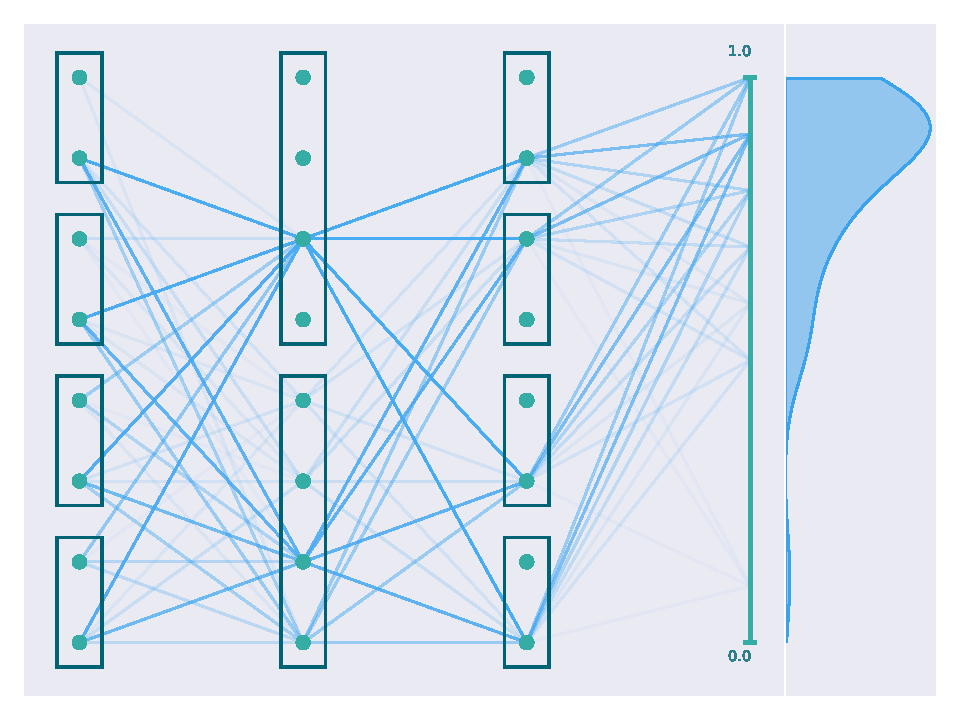
\includegraphics[width=\textwidth]{Figures/MLResults/NN/NetworkVis/AfterTrainingSig200300.pdf}
        \vspace{-0.5cm}
        \caption{}
        \label{fig:ATrainingSig200300}
    \end{subfigure}
    }
    \caption[A calculated visualization of the activation of a three layer maxout network, after training and displaying
    the results for two signal with each their own mass combination.]{A calculated visualization of a trained maxout network 
    with three hidden layers. The lines represent the path through the nodes with the largest activation in their respective
    unit. The bolder the line the more frequently the path is used. The distribution on the far right represent the output 
    distribution. The figure to the left (\ref{fig:ATrainingSig50250}) is a result of signal with masses $\{50,250\}_{GeV}$ 
    and the right (\ref{fig:ATrainingSig200300}) with masses $\{200,300\}_{GeV}$.}
    \label{fig:NetVisSigComp}
\end{figure}
Ideally, we would want the model to not only be able to separate the signal from the background, but do so in 
a way which allows the network to store the different patterns within the signal. In section \ref{subsubsec:Channel-Out},
I described this ability as long-term memory. One way to implement long-term memory is through a high number of parameters.
However through the \ac{LWTA} layers we can achieve the same through specific paths. To study this I have created similar 
figures as discussed in the paragraphs above, but this time only including results from applying the network on one mass combination. 
Figures \ref{fig:ATrainingSig50250} and \ref{fig:ATrainingSig200300} present the results for the mass combinations 
$\{50,250\}_{GeV}$, and $\{200,300\}_{GeV}$ respectively.
By comparing the figures, we see a small but noticeable difference in paths. Again the middle hidden layer seems to be 
the differentiating factor. To highlight the differences, I have included a cutout, comparing the first and second node in the bottom unit 
for the middle layer of both figures, \ref{fig:ATrainingSig50250Zoom} and \ref{fig:ATrainingSig200300Zoom}.
By studying the cutouts, we can discern that the maxout layer allows the model to discriminate both background from signal, 
and different variations of the signal through an increase in long-term memory. We can conclude that the maxout layer not only 
applies a form of regularization, but also increases the long-term memory of the model through pattern-specific paths through the network.\\
\begin{figure}
    \makebox[\linewidth][c]{%
    \centering
    \hfill
    \hfill
    \begin{subfigure}{.09\textwidth}
        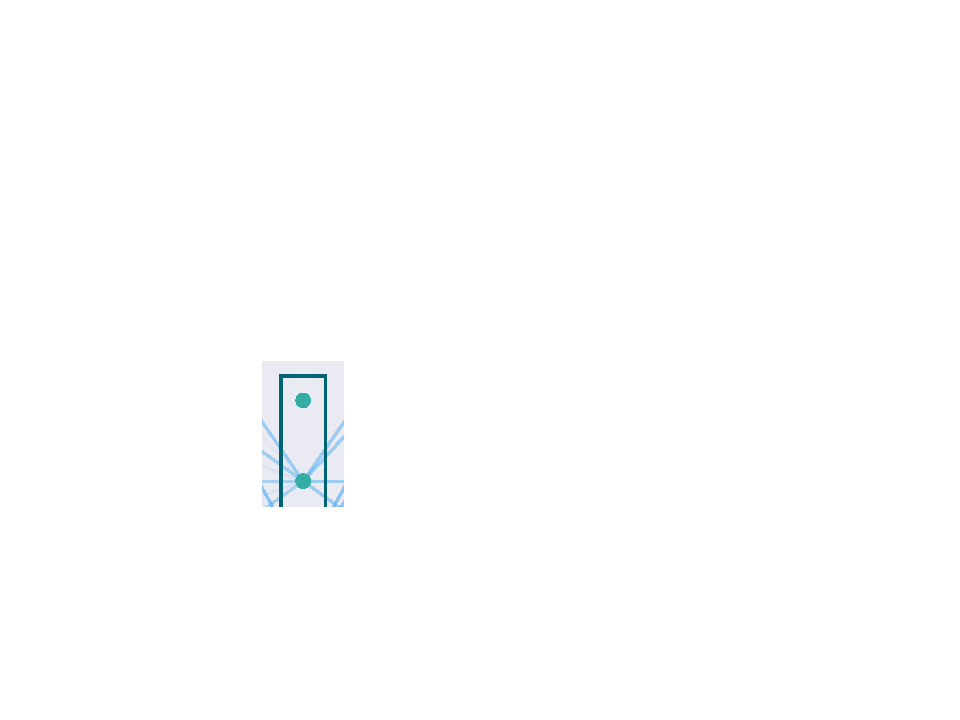
\includegraphics[width=\textwidth]{Figures/MLResults/NN/NetworkVis/AfterTrainingSig50250Zoom.pdf}
        \vspace{-0.5cm}
        \caption{}
        \label{fig:ATrainingSig50250Zoom}
    \end{subfigure}
    \hfill
    \begin{subfigure}{.094\textwidth}
        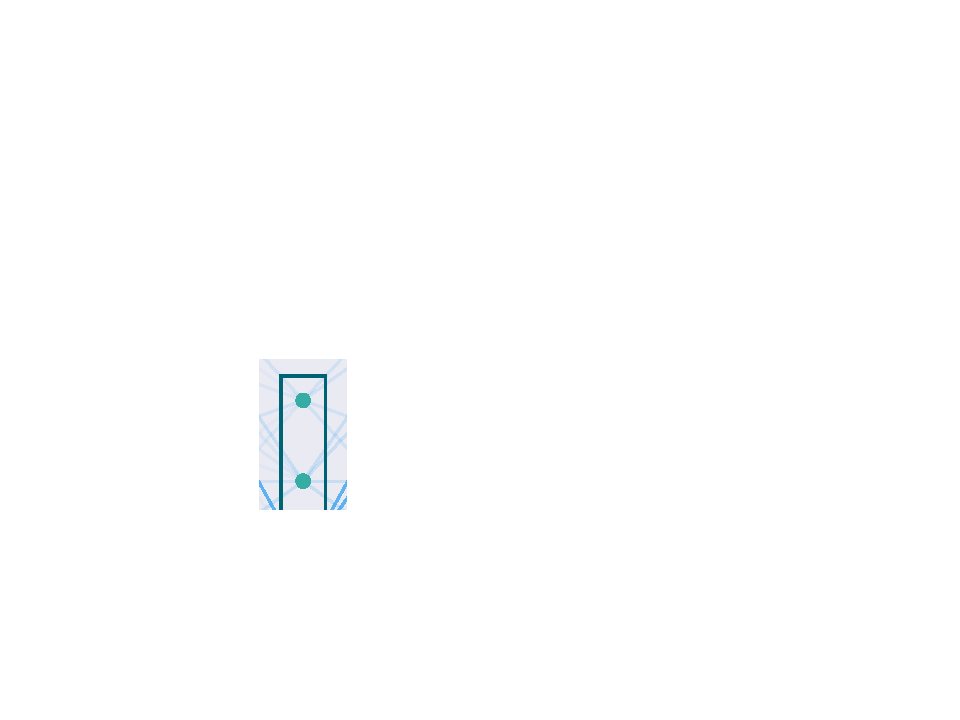
\includegraphics[width=\textwidth]{Figures/MLResults/NN/NetworkVis/AfterTrainingSig200300Zoom.pdf}
        \vspace{-0.5cm}
        \caption{}
        \label{fig:ATrainingSig200300Zoom}
    \end{subfigure}
    \hfill
    \hfill
    }
    \caption[A calculated visualization of the activation of a three layer maxout network, after training and displaying the
    the results for two signal with each their own mass combination, highlighting the difference between two specific nodes.]{
    A cut-out of the fifth and sixth node (counting from the top) in the second hidden layer, activated 
    by the signal with masses $\{50,250\}_{GeV}$ \ref{fig:ATrainingSig50250Zoom} and 
    $\{200,300\}_{GeV}$ \ref{fig:ATrainingSig200300Zoom}.}
    \label{fig:NetVisZoom}
\end{figure}
Finally, I wanted to compare the activations of the maxout model, to the activation of the \ac{SCO} model. In section \ref{subsubsec:stochchannelout},
I stated that the inspiration behind the \ac{SCO} was to elevate the channel-out method in a way which reduced complex co-adaptation among neighboring
nodes. In figure \ref{fig:NetDistSCO}, I included a visualization of the activation of a three layer \ac{SCO} network before (\ref{fig:BTrainingSCO}) 
and after (\ref{fig:ATrainingSCO}) training. By comparing the activations from the \ac{SCO} layers to maxout, we can discern that the \ac{SCO} behaves
exactly as intended. In the figures visualizing the maxout layer (\ref{fig:NetDist1}), we can observe that several of the nodes which are not activated 
before training, are left dormant even after training. In comparison, the \ac{SCO} layers display a far more balanced activation, and exhibits no signs 
of complex co-adaptation. 
\begin{figure}[H]
    \makebox[\linewidth][c]{%
    \centering
    \begin{subfigure}{.6\textwidth}
        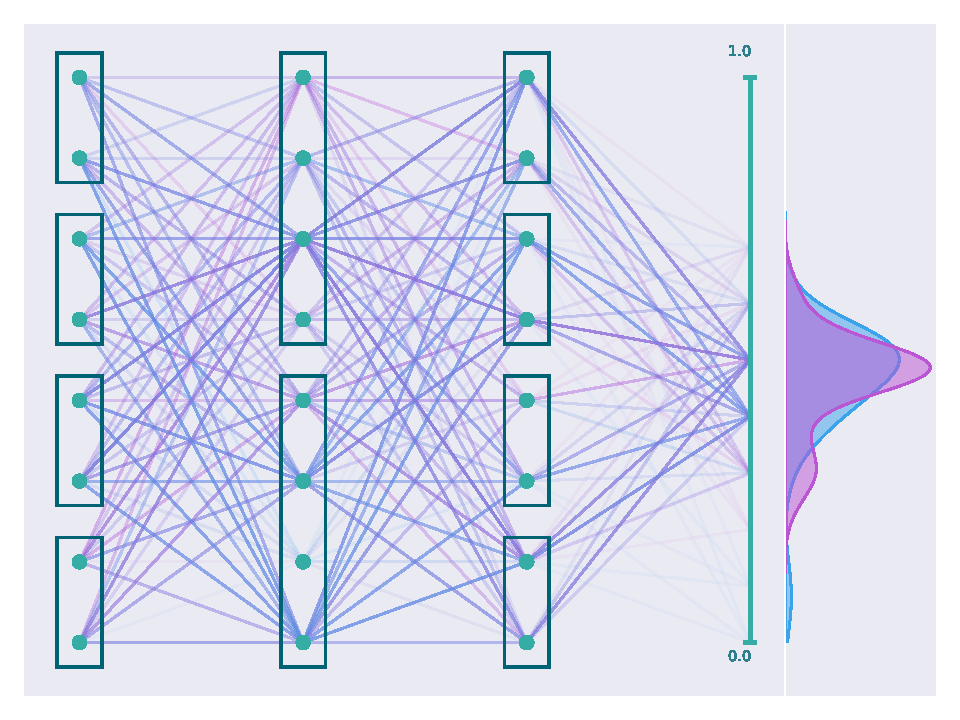
\includegraphics[width=\textwidth]{Figures/MLResults/NN/NetworkVis/SCO/BeforeTraining.pdf}
        \caption{}
        \label{fig:BTrainingSCO}
    \end{subfigure}
    \hfill
    \begin{subfigure}{.6\textwidth}
        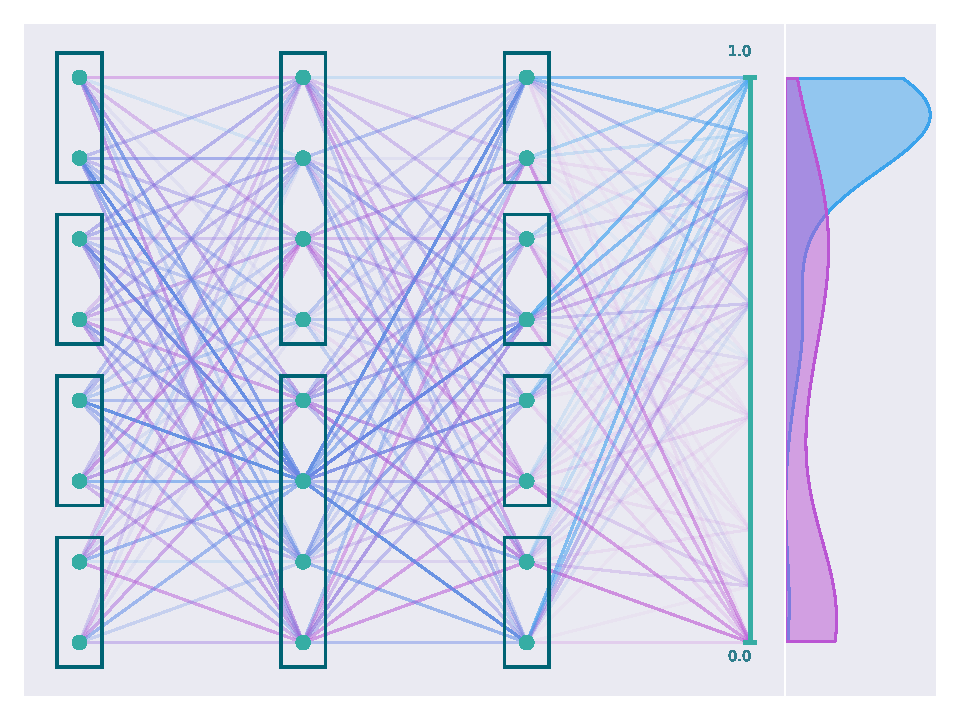
\includegraphics[width=\textwidth]{Figures/MLResults/NN/NetworkVis/SCO/AfterTraining.pdf}
        \caption{}
        \label{fig:ATrainingSCO}
    \end{subfigure}
    }
    \caption[A calculated visualization of the activation of a three layer \acs{SCO} network, after training and displaying the
    signal and background separately.]{A calculated visualization of a three layer \acs{SCO} network. The lines represent the path 
    through the nodes with the largest activation in their respective unit. The bolder the line the more frequently the path is used. 
    The distribution on the far right represent the output distribution.
    The figure to the left (\ref{fig:BTrainingSCO}) is the result before training and the figure to right (\ref{fig:ATrainingSCO})
    is after.} 
    \label{fig:NetDistSCO}
\end{figure}
\subsection{Training History and Overfitting}\label{subsec:Overfitting}
In section \ref{sec:Regularization} I described how creating ensembles of networks is a form of regularization. Therefore,
it is of interest to study the relationship between performance on the training set and the validation set for our ensemble 
methods. In figure \ref{fig:History} I drew plots displaying the performance on the training and validation scores after each 
epoch (50 in total), as measured in \ac{AUC} for both a dense \ac{NN} (\ref{fig:NNHist}) and maxout (\ref{fig:MaxOutHist}).
\\ 
In figure \ref{fig:NNHist} we can observe that an ordinary dense \ac{NN} reaches a maximum in performance for the validation set after only 
a couple of epochs. This peak is then followed by a quick drop in performance, while the training set increases in performance. 
The drop in performance for the validation set and increase in performance for the training set is a sure sign of overfitting. 
\\
In figure \ref{fig:MaxOutHist} we observe that an ensemble method (in this case the maxout) displays a different training history. For the first 
10 epochs the model increases in performance for both data sets. After this, the validation set does not decrease in performance, but 
simply holds stable while the training set increases. This is a sign that the model is not experiencing overfitting. Furthermore, the 
training history of the maxout model raises an interesting point. From experience I know that the maxout model reaches a peak in performance
on the validation set after approximately 15-20 epochs. Given that the performance after this is stable, it is plausible that continuing 
training will not worsen the performance or lead to overfitting, but rather improve. This is definitely an interesting possibility
for the \ac{LWTA} layers, but will not be studied in this thesis due to time constraints.
\\
In section \ref{subsec:TrainingStrategy}, I discussed the training strategy used when training all models in this analysis. I mentioned 
the implementation of an early stopping criterion which makes sure that the model continues to train only as long as the performance on the 
validation data set increases. By studying the subfigures in figure \ref{fig:History}, we can deduce that the ensemble methods will not only 
be able to avoid overfitting, but will as a consequence be allowed to train much longer than the other models.
\begin{figure}[H]
    \makebox[\linewidth][c]{%
    \centering
    \begin{subfigure}{.45\textwidth}
        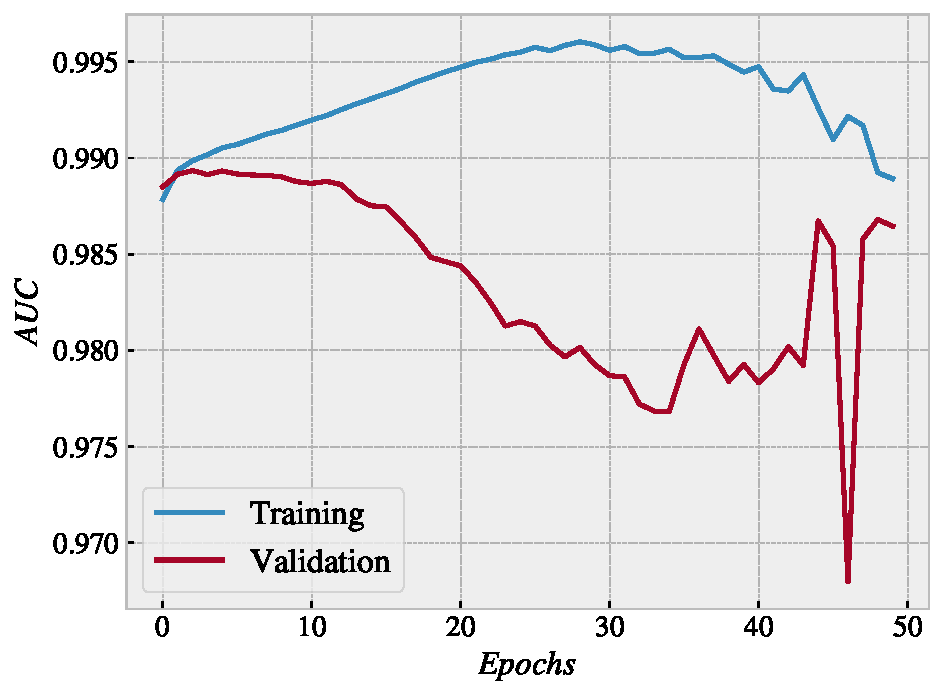
\includegraphics[width=\textwidth]{Figures/MLResults/NN/SUSY/History/NNHistory.pdf}
        \caption{}
        \label{fig:NNHist}
    \end{subfigure}
    \begin{subfigure}{.45\textwidth}
        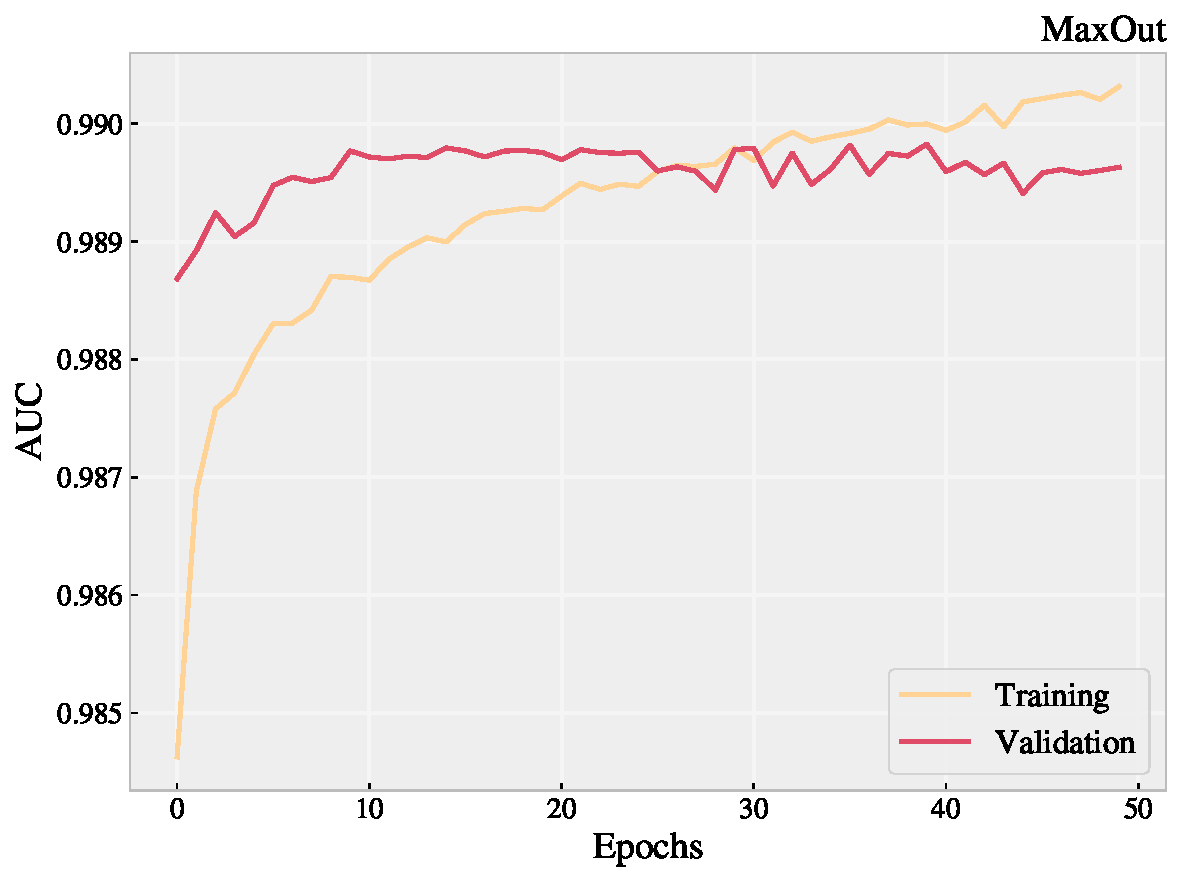
\includegraphics[width=\textwidth]{Figures/MLResults/NN/SUSY/History/MaxOutHistory.pdf}
        \caption{}
        \label{fig:MaxOutHist}
    \end{subfigure}
    }
    \caption[A plot comparing the \acs{AUC} score made after each epoch on both the training and validation set, between a dense \acs{NN} 
    and maxout model.]{A plot displaying the \acs{AUC} score made after each epoch on both the training and validation set. 
    Figure \ref{fig:NNHist} shows the results from the dense \ac{NN} and figure \ref{fig:MaxOutHist} shows
    the results from a maxout network.}
    \label{fig:History}
\end{figure}
\subsection{Comparing Achieved Sensitivity between Ensemble Methods}
In this section I will present and discuss the performance of the three different networks discussed in section 
\ref{subsec:Ensembles}, channel-out, \ac{SCO} and maxout. The results presented in this section were made using the
original signal set (see section \ref{subsec:signal}), the training strategy described in section \ref{subsec:TrainingStrategy}
and the architectures described in section \ref{subsec:arch}.
\\
In figure \ref{fig:MaxOutGridSig} I present the achieved sensitivity of the maxout model using the original signal set. 
The grid shows the same trends as the previous models, i.e. the preference in the higher statistics mass combinations. By comparing 
the results from the maxout model to the deep, dense network presented in figure \ref{fig:NNGridSig}, we discern that the dense 
network outperforms the maxout model (ever so slightly) for the higher statistic mass combinations. It is plausible that this is due 
to the difference in depth. The dense network utilizes 3 hidden layers of 600 nodes each, while the maxout, although built with the 
same architecture, only utilizes 200 nodes per layer when propagating input through the network. This could result in the dense network 
being able to more deeply tune for the patterns in the higher statistics combinations.
\\
However, the most interesting result for the maxout model, is its ability to tune for all mass combinations. Although the dense network
outperformed the maxout model for the high statistics combinations, the maxout model outperformed the dense for most other combination (26 of 
the 30 possible mass points). This result can be credited to two factors. The first being maxout's effect as a form of regularization. In the previous 
section (see section \ref{subsec:Overfitting}), I presented how, maxout, through its regularization abilities, is able to 
uphold the early stopping criteria for a larger number of epochs. The second factor is maxout's innate long-term memory which was studied
in section \ref{subsec:Viz}. From figure \ref{fig:MaxOutGridSig}, we are able to deduce that although the maxout model is not able to tune 
to the same depth for the lower masses, it is able to achieve a large level of generalizability through reducing overfitting and increasing 
long-term memory.\\
\begin{figure}
    \makebox[\linewidth][c]{%
    \centering
    \begin{subfigure}{.65\textwidth}
        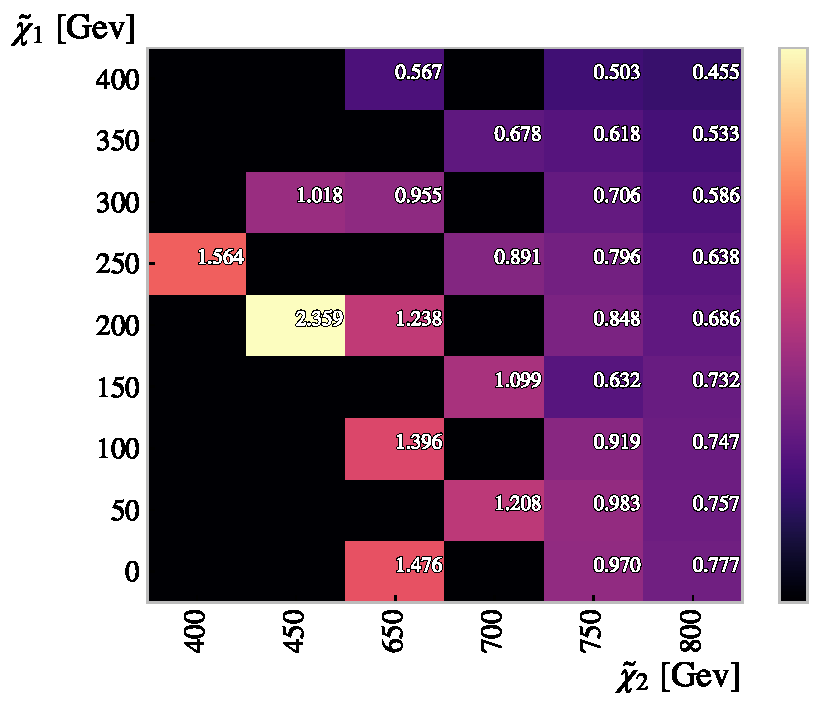
\includegraphics[width=\textwidth]{Figures/MLResults/NN/SUSY/Grid/MaxOutGridSig.pdf}
    \end{subfigure}
    }
    \caption{A grid displaying the expected significance on the original signal set, using the signal region 
    created by the maxout network.}
    \label{fig:MaxOutGridSig}
\end{figure}
In appendix \ref{appendix:Ensembles} I have included grids displaying the achieved sensitivity for both channel-out and \ac{SCO}. Both 
models demonstrate similar performance to the maxout layer. To compare the three methods I created a 'pie-plot'. A 'pie-plot' 
compares the achieved sensitivity between several models and displays the results for each individual mass combination.  In figure 
\ref{fig:EnsembleComp} I present the 'pie-plot' comparing maxout, channel-out and \ac{SCO}. Each mass combination includes a pie, where 
the size of each 'slice' represents the relative size of the significance compared to the other methods. For example, if a slice occupies 
half of the pie, then the method corresponding to that slice achieved a significance equal to the sum of the significance of the other methods.
The color surrounding each pie marks which method achieved the highest sensitivity for the respective combination.
\\
By studying the 'pie-plot' in figure \ref{fig:EnsembleComp}, we can deduce that maxout model outperforms the other two in most of the mass 
combination (24 out of the 30 mass points). From the sizes of each slice, we can deduce that all three models seem relatively equal in performance, maxout only 
outperforming the others by a small fraction. The most interesting observation from the 'pie-plot' is the performance from the \ac{SCO}, as 
this model was in-part created by me. Except the mass combinations where maxout was the most sensitive, \ac{SCO} was the best performing model. 
Most interestingly, it outperformed the channel-out model, which is the model most similar to \ac{SCO}, in 9 out of the 30 mass point (see figure \ref{fig:SCOCO}). 
In hindsight, I believe that by removing the \ac{SCO} during prediction (similar to what is done for dropout), the \ac{SCO} layer would greatly 
approve in performance, on a count of the fact that the performance on each event is dependent on the random choice of unit for that prediction.
This means it is possible that upon prediction, a data point is sent through a path which has never been chosen during training. 
Nonetheless, this analysis is an indicator that although the maxout model was the highest performing model, the \ac{SCO} layer shows 
great promise and should be further explored in further analysis. 
\begin{figure}
    \makebox[\linewidth][c]{%
    \centering
    \begin{subfigure}{.75\textwidth}
        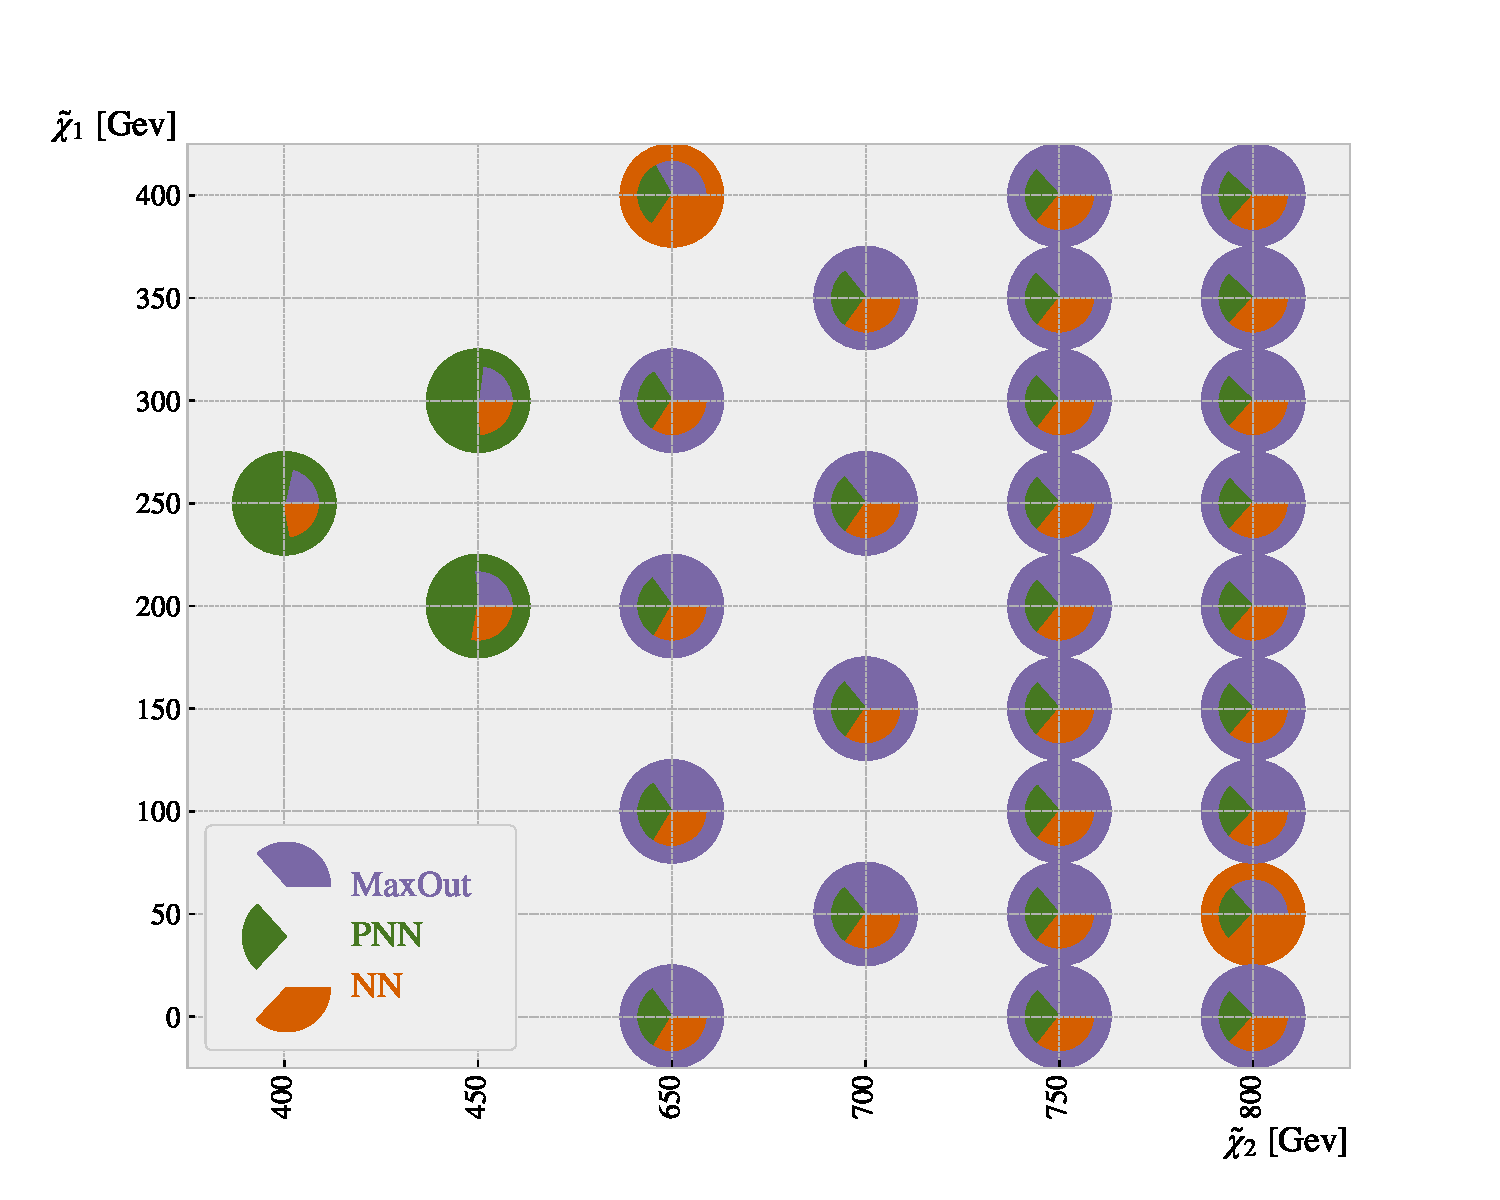
\includegraphics[width=\textwidth]{Figures/MLResults/NN/SUSY/Comparison/EnsemblesNetworkComp.pdf}
    \end{subfigure}
    }
    \caption[A sensitivity comparison between the ensemble networks (maxout, \acs{SCO}, channel-Out) on the original 
    signal data.]{A sensitivity comparison between the ensemble networks (maxout, \acs{SCO}, channel-Out) on the original 
    signal data. The size of each slice represents the relative size of the significance and the color around each 
    point displays the method with the largest sensitivity for the respective combination.}
    \label{fig:EnsembleComp}
\end{figure}


\section{Parametrized Neural Network}
\subsection{Discriminating Masses}
When introducing the \ac{PNN} in section \ref{subsec:PNN}, I mentioned that by including the masses of the introduced particles
in the feature set, we motivate and individualistic tuning for each mass combination in the signal set. To test if this is indeed what 
happens, I will in this section present results where I manually assign different mass combinations the same parameter. The hope 
is that if indeed the \ac{PNN} has been able to tune individually for each mass combination, then the \ac{PNN} should perform best 
when the events are correctly labeled compared to when they are not. 
\\
In figure \ref{fig:PNN50250Dist} I have drawn the distribution of the output from the trained \ac{PNN} architecture 
(see section \ref{subsec:PNNArch}). The model was trained using the full statistics signal set. In figure \ref{fig:PNN50250Dist},
4 signals have been included; ($\tilde{\chi}_1=50$, $\tilde{\chi}_2=250$GeV), ($\tilde{\chi}_1=100$, $\tilde{\chi}_2=200$GeV), 
($\tilde{\chi}_1=200$, $\tilde{\chi}_2=300$GeV) and ($\tilde{\chi}_1=150$, $\tilde{\chi}_2=250$GeV). All data, including 
both signal and background were given the labels of $50$ and $250$ (corresponding to the masses $\tilde{\chi}_1=50$, $\tilde{\chi}_2=250$GeV). 
In figure \ref{fig:PNN50250Dist} the full output range is included, whereas in figure \ref{fig:PNN50250Dist_95} only the output in the 
range $[0.975-1]$ has been included. In both figures, it is evident that all mass combinations have been effectively separated from the background,
even for the combinations which are given the wrong parameter. Nevertheless, upon close study of the figures and the corresponding legends, we can deduce that
the signal which is given the correct label is also the signal which has the highest percentage of conserved events when applying a simple cut off 
$0.975$\footnote{This is further evident when studying the efficiency rates in table \ref{table:PNNSigComp}.}.\\
\begin{figure}
    \makebox[0.95\linewidth][c]{%
    \centering
    \begin{subfigure}{.5\textwidth}
        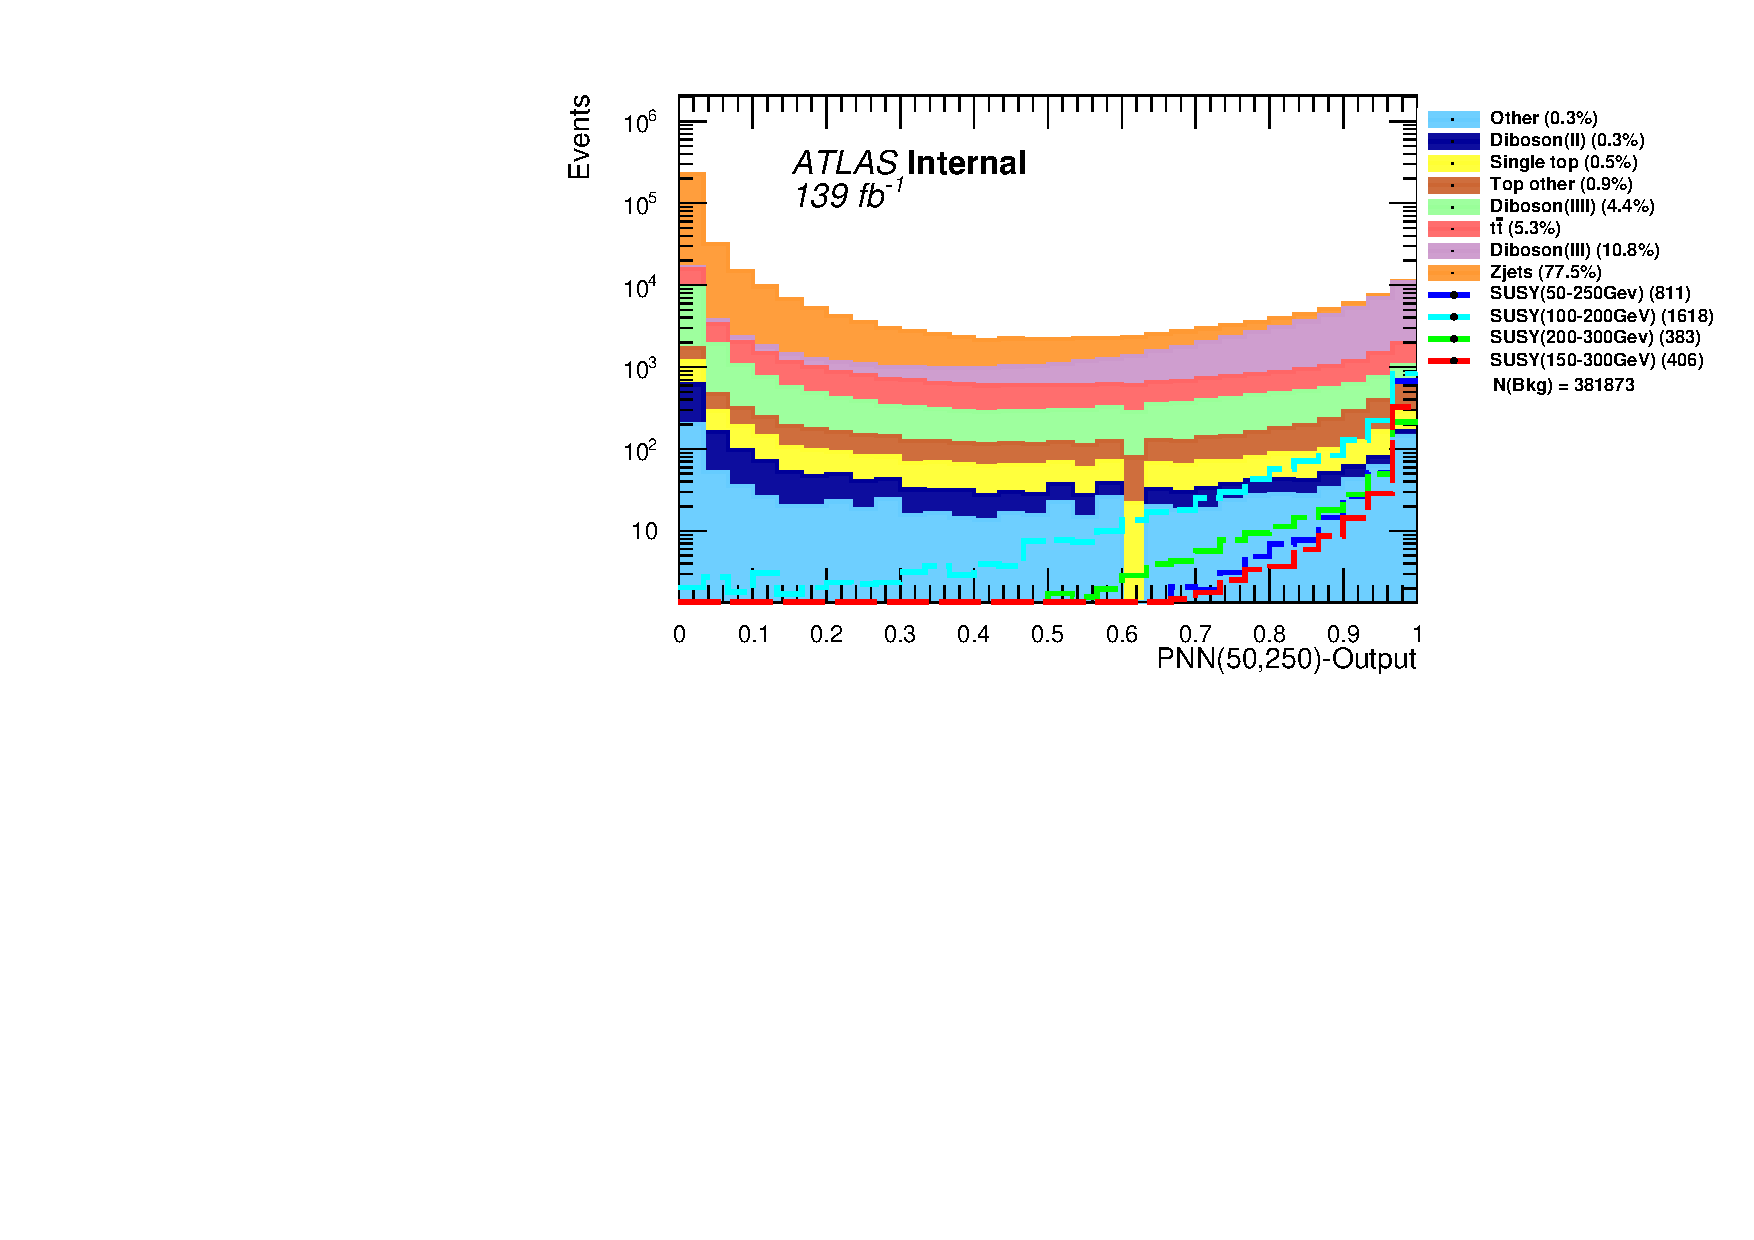
\includegraphics[width=\textwidth]{Figures/MLResults/NN/SUSY/MLDist/PNNDistTest/PNN50250Dist.pdf}
        \caption{}
        \label{fig:PNN50250Dist}
    \end{subfigure}
    \hfill
    \begin{subfigure}{.5\textwidth}
        \includegraphics[width=\textwidth]{Figures/MLResults/NN/SUSY/MLDist/PNNDistTest/PNN50250Dist_C7.pdf}
        \caption{}
        \label{fig:PNN50250Dist_95}
    \end{subfigure}
    }
    \caption{The output distribution from a trained \ac{PNN} model for the background and signals with 4 different mass combinations:
    ($\tilde{\chi}_1=50$, $\tilde{\chi}_2=250$GeV), ($\tilde{\chi}_1=100$, $\tilde{\chi}_2=200$GeV), 
    ($\tilde{\chi}_1=200$, $\tilde{\chi}_2=300$GeV) and ($\tilde{\chi}_1=150$, $\tilde{\chi}_2=250$GeV), and where all the data were given the 
    parameter features of ($\tilde{\chi}_1=50$, $\tilde{\chi}_2=250$GeV). The figure includes the full output range (\ref{fig:PNN50250Dist}) 
    and the output ranging from 0.975-1.00 (\ref{fig:PNN50250Dist_95}).}
    \label{fig:PNN50250}
\end{figure}
In section \ref{sec:XGBoost} I presented results indicating that some signals were easier to separate from background than others. This leads me to the 
question; did the \ac{PNN} perform better on the signal with ($\tilde{\chi}_1=50$, $\tilde{\chi}_2=250$GeV) because of the labeling, or simply
because this particular signal was easier to separate. To answer this question I conducted a second test. In figure \ref{fig:PNN200300DistComp} 
I repeated the analysis described in the paragraphs above, but where all the signals were given the label ($\tilde{\chi}_1=200$, $\tilde{\chi}_2=300$GeV).
Similarly to the previous results, I drew the output for the full output range (\ref{fig:PNN200300Dist}) and after a cutoff off $0.975$ (\ref{fig:PNN50250Dist_95}).
Via the examination of the two figures, we can indeed see that my assumption was right. Despite the fact that events with masses equal to $\tilde{\chi}_1=50$ and $\tilde{\chi}_2=250$GeV
are given the wrong parameter, the \ac{PNN} achieves the highest efficiency when predicting on the aforementioned events. \\
\begin{figure}
    \makebox[0.95\linewidth][c]{%
    \centering
    \begin{subfigure}{.5\textwidth}
        \includegraphics[width=\textwidth]{Figures/MLResults/NN/SUSY/MLDist/PNNDistTest/PNN200300Dist.pdf}
        \caption{}
        \label{fig:PNN200300Dist}
    \end{subfigure}
    \hfill
    \begin{subfigure}{.5\textwidth}
        \includegraphics[width=\textwidth]{Figures/MLResults/NN/SUSY/MLDist/PNNDistTest/PNN200300Dist_C7.pdf}
        \caption{}
        \label{fig:PNN200300Dist_95}
    \end{subfigure}
    }
    \caption{The output distribution from a trained \ac{PNN} model for the background and signals with 4 different mass combinations:
    ($\tilde{\chi}_1=50$, $\tilde{\chi}_2=250$GeV), ($\tilde{\chi}_1=100$, $\tilde{\chi}_2=200$GeV), 
    ($\tilde{\chi}_1=200$, $\tilde{\chi}_2=300$GeV) and ($\tilde{\chi}_1=150$, $\tilde{\chi}_2=250$GeV), and where all the data were given the 
    parameter features of ($\tilde{\chi}_1=200$, $\tilde{\chi}_2=300$GeV). The figure includes the full output range (\ref{fig:PNN50250Dist}) 
    and the output ranging from 0.975-1.00 (\ref{fig:PNN50250Dist_95}).}
    \label{fig:PNN200300DistComp}
\end{figure}
To further study this result, I created a table of the efficiencies of each mass combination for both results, after applying a simple cut of $0.975$. The results are presented in 
table \ref{table:PNNSigComp}. It is evident from table \ref{table:PNNSigComp} that the \ac{PNN} achieves the highest performance when events are given the correct label, 
although not by much. In the events with masses $\tilde{\chi}_1=50$ and  $\tilde{\chi}_2=250$GeV, the efficiency improved by a little over $3\%$, while the event with masses 
$\tilde{\chi}_1=200$ and $\tilde{\chi}_2=300$GeV, improved efficiency by almost $10\%$. Another interesting observation is that events with ($\tilde{\chi}_1=100$, $\tilde{\chi}_2=200$GeV) seem to prefer the label of 
($\tilde{\chi}_1=200$, $\tilde{\chi}_2=300$GeV) over that of ($\tilde{\chi}_1=150$, $\tilde{\chi}_2=250$GeV), despite the latter mass combination being closer 
in mass. A possible explanation is that the difference in mass ($\Delta m = |m_{\tilde{\chi}_1} - m_{\tilde{\chi}_2}|$), influences the trends in the data, similarly 
to what we saw that size of mass does. Regardless, from \ref{table:PNNSigComp}, we can deduce that the \ac{PNN} does in fact discriminate between mass combinations 
and tune for them independently.
\begin{table}
    \centering
    $
    \begin{array}{ccccc}
        \hline \text { \backslashbox{\textbf{Label}}{\textbf{Channel}} }  & \text {$(50,250)$}& \text {$(100,200)$} & \text {$(150,300)$} & \text {$(200,300)$} \\
        \hline\text {$(50,250)$}   & \text { $\bf{80.8}\%$ } & \text { $45.8\%$ } & \text { $\bf{77.5}\%$ } & \text { $50.1\%$ } \\
        \hline\text {$(200,300)$}   & \text { $77.3\%$ } & \text { $\bf{54.6}\%$ } & \text { $76.3\%$ } & \text { $\bf{59.0}\%$ } \\
        \hline
    \end{array}
    $
    \caption{A listing of the remaining procentage of each mass combination in the output range 0.975-1.00 using the 
    labels ($\tilde{\chi}_1=50$, $\tilde{\chi}_2=250$GeV) and ($\tilde{\chi}_1=200$, $\tilde{\chi}_2=300$GeV) respectively.}
    \label{table:PNNSigComp}
\end{table}

\subsection{Sensitivity Result}
In this section I will present the achieved sensitivity by the \ac{PNN} on the original signal set. In figure \ref{fig:PNNGridSig}, I present a grid displaying the sensitivity 
of the \ac{PNN} on the original signal set. Similarly to the previous models', the figure indicates that the \ac{PNN} is able to achieve a much higher sensitivity on the lower
masses. The most notable difference to the previous models, is the span of values for the significance. The \ac{PNN} almost doubles the highest significance achieved by any previous model
(from 2.44 to 4.14), and simultaneously achieves the lowest significance (now 0.30). The most probable explanation to this result is the distribution of parameters for the background. 
In section \ref{subsec:PNN}, I described how the background is randomly assigned parameters such that the percentage of background with a given parameter is equal to the percentage 
of the signal with the same parameter. In other words, the higher the statistics for a given mass combination, the higher the amount of background will be "linked" to it. Inn the 
same section I also described the hope that the parameters would shift the output from the initial layer in a way that motivates individualistic training. If this is 
true\footnote{For a network of this depth, it is very hard to explain what happens during training, which explains the passive statement.} it means that masses with larger statistics, 
are given larger amounts of background to train with. This could explain the uneven performance by the \ac{PNN}. \\
\begin{figure} 
    \makebox[\linewidth][c]{%
    \centering
    \begin{subfigure}{.65\textwidth}
        \includegraphics[width=\textwidth]{Figures/MLResults/NN/SUSY/Grid/PNNGridSig.pdf}
    \end{subfigure}
    }
    \caption{A grid displaying the achieved significance on the original signal set, using the signal region 
    created by the \ac{PNN} network.}
    \label{fig:PNNGridSig}
\end{figure}
In this analysis I choose to follow the methodology described in the article by Baldi et al. \cite{PNN}, but other variants of the \ac{PNN} could 
be of interest in future studies. An alternative to the current setup for distributing parameters to the background, is to distribute the parameters evenly. 
In other words, for N different mass combinations, each set of parameters will be distributed to 1/N parts of the background. This would most likely produce a
more balanced result. I considered using an even approach, but found that the current setup was more aligned with the rest of the analysis where a 1-1, signal-
background ratio approach has been made\footnote{In section \ref{subsec:TraVal} I discuss how I have chosen to scale the weights such that sum of the weights of 
the background is equal to the sum of the weights of the signal.}. The more interesting alternative would be to assign the background most similar to a given mass 
combination\footnote{By most similar, I refer to the background with the largest overlap in the feature space to the signal.}, the same parameters. This would 
focus the training of the \ac{PNN} on the set of events which should be hardest to separate. One approach to determine which events are deemed 'most similar' to a 
combination, is to apply a prior \ac{ML} analysis with a simple \ac{BDT} or dense \ac{NN}. Due to time constraints of this thesis, I decided not to test this 
approach, but would be an interesting area to explore.
\section{Remarks on Comparison between Models on Original Signal Set}
So far in the thesis I have presented results from two branches of \ac{ML}, \acf{BDT} and \acf{NN}. In the case of the latter, I tested
three further variations, a dense \ac{NN}, ensemble networks and \ac{PNN}. In figure \ref{fig:GenPlussXGB} I have drawn a pie-plot comparing 
the sensitivity on the original signal set for the four different models. By assessing figure \ref{fig:GenPlussXGB}, we can deduce that the 
maxout network outperforms all other models in most mass combinations (24/30), although not by much. Additionally, we can discern that the \ac{PNN}
is far more sensitive than the other models for higher statistics mass combinations, and underperforms for low statistic mass combinations.
This indicates that the \ac{PNN} is able to train much deeper than the maxout model, but struggles to uphold performance for a diverse signal set. 
The long term memory of the maxout layer, allows the model to train relatively evenly for all trends in the signal set, but at the cost of never 
training to the same depth as the \ac{PNN}
\\
On the other hand, the XGBoost model is outperformed in all but one combination, implying that the networks are more ideal for this analysis. 
It is worth noting however, that not at a lot of time was spent improving the XGBoost model. While for the networks, I experimented with different layers and 
tested for different architectures, no effort was put in deciding the architecture of the XGBoost. Likewise, the solution to the negative weights (see 
section \ref{subsec:negWeights}) could by all means be optimized if given more attention. Therefore, it is worth saying that the results in this analysis
do not imply that deep networks are a better analysis tool for \ac{BSM} searches than \ac{BDT}'s, but rather exemplify the advanced capabilities of deep networks.
\begin{figure}
    \makebox[\linewidth][c]{%
    \centering
    \begin{subfigure}{.75\textwidth}
        \includegraphics[width=\textwidth]{Figures/MLResults/NN/SUSY/Comparison/GenPlussXGBNetworkComp.pdf}
    \end{subfigure}
    }
    \caption{A sensitivity comparison between a dense \ac{NN}, \ac{PNN}, maxout and XGBoost on the original 
    signal data. The size of the "pie" represents the relative size of the significance and the color around each 
    point displays the method with the largest sensitivity for the respective combination.}
    \label{fig:GenPlussXGB}
\end{figure}

\section{Increasing Sensitivity through PCA}
So far in the analysis, all features have been given an equal weighting in the beginning of training,
But, as mentioned in section \ref{sec:MLHEP}, not all features contribute to an effective signal 
region. In section \ref{subsec:PCA}, I explained how through the use of \ac{PCA}, we are able to 
create a new set of features which can be ordered by amount of variance. In this way, we can reduce
the dimensionality of the data set, while at the same time preserving most of the variance. Inn this 
section I will present the results of training on a data set which has gone through such a \ac{PCA}.
\\
In this analysis I performed a \ac{PCA} on the data set, and demanded that $99.99\%$ of the variance 
should be preserved. In doing so, 5 features were removed. 
\subsection*{NN and PCA}

\begin{figure}
    \makebox[\linewidth][c]{%
    \centering
    \begin{subfigure}{.65\textwidth}
        \includegraphics[width=\textwidth]{Figures/MLResults/NN/SUSY/Comparison/NNPCANetworkComp.pdf}
    \end{subfigure}
    }
    \caption{A grid displaying the achieved significance on the original signal set, using the signal region 
    created by the \ac{NN} network. A \ac{PCA} analysis has been applied to the data being utilized in this result.}
    \label{fig:NNPCAComp}
\end{figure}

\subsection*{MaxOut Network and PCA}

\begin{figure}
    \makebox[\linewidth][c]{%
    \centering
    \begin{subfigure}{.65\textwidth}
        \includegraphics[width=\textwidth]{Figures/MLResults/NN/SUSY/Comparison/MaxOutPCANetworkComp.pdf}
    \end{subfigure}
    }
    \caption{A grid displaying the achieved significance on the original signal set, using the signal region 
    created by the \ac{NN} network. A \ac{PCA} analysis has been applied to the data being utilized in this result.}
    \label{fig:MaxOutPCAComp}
\end{figure}
\subsection*{PNN and PCA}

\begin{figure}
    \makebox[\linewidth][c]{%
    \centering
    \begin{subfigure}{.65\textwidth}
        \includegraphics[width=\textwidth]{Figures/MLResults/NN/SUSY/Comparison/PNNPCANetworkComp.pdf}
    \end{subfigure}
    }
    \caption{A grid displaying the achieved significance on the original signal set, using the signal region 
    created by the \ac{NN} network. A \ac{PCA} analysis has been applied to the data being utilized in this result.}
    \label{fig:PNNPCAComp}
\end{figure}

\begin{figure}
    \makebox[\linewidth][c]{%
    \centering
    \begin{subfigure}{.65\textwidth}
        \includegraphics[width=\textwidth]{Figures/MLResults/NN/SUSY/Comparison/PCANetworkComp.pdf}
    \end{subfigure}
    }
    \caption{A grid displaying the achieved significance on the original signal set, using the signal region 
    created by the \ac{NN} network. A \ac{PCA} analysis has been applied to the data being utilized in this result.}
    \label{fig:PCAComp}
\end{figure}

\section{Comparing Models on Full Statistics Signal}
So far in the analysis I have only tested on a subset of the signal, which I have called the original signal set. In this section 
I will extend my search to include the full signal set displayed in figure \ref{fig:nrSignal}. The full signal set consists of 89 mass 
combinations compared to the original 30, and extends the mass ranges to $\tilde{\chi}_1 \in [0-400]GeV$ and $\tilde{\chi}_2 \in [200-800]GeV$.
In the figures to come, I have included a turquoise band around all combinations with a significance of over 1.64 (see section \ref{subsec:Sensitivity}).
When comparing the results, we are not only interested in how sensitive the models are for each combination individually, but also with how many combinations 
they were able to achieve a sensitivity of over 1.64. However, similarly to previous results, the significance does not include any uncertainty.
\\
I will not apply all previously tested models to the full statistics signal set. Instead, I will only apply the models I found most ideal for this analysis, based 
on the tests performed in the previous sections. I decided to choose one model from each "type"\footnote{By network type, I am referring to either the ordinary dense network, the 
\ac{PNN} or an ensemble. } of network. Based on the results in section \ref{sec:Ensemble}, where I compared the different ensemble methods, I found the maxout model to be 
the top performer. Likewise, in section \ref{sec:PCA} I found that both maxout and the \ac{PNN}, preferred to utilize data with a \ac{PCA}. Therefore, I will utilize the maxout model 
and \ac{PNN} model defined in section \ref{subsec:arch}, with the use of \ac{PCA}. Finally, I will include the ordinary dense \ac{NN} for the sake of diversity.
\\
In figure \ref{fig:NN_FS_MLMGridSig}, I have drawn a grid displaying the sensitivity of an ordinary dense \ac{NN}, on the full statistics signal set. Again, we observe that higher statistics
mass combinations, result in a higher significance. Additionally, the dense \ac{NN} was able to achieve a sufficient significance for over 38 mass combinations, all between the ranges of 
$\tilde{\chi}_1 \in [0-250]GeV$ and $\tilde{\chi}_2 \in [200-600]GeV$. What is even more interesting, is that by comparing the results on the full set with the results on the original 
set (see figure \ref{fig:NNGridSig}), we notice that the network was able to improve its sensitivity on every single mass combination from the original signal set. This is yet another 
indication that the deep networks are able to exploit overlapping regions in the feature space between nearby combinations.\\
\begin{figure}
    \makebox[\linewidth][c]{%
    \centering
    \begin{subfigure}{.85\textwidth}
        \includegraphics[width=\textwidth]{Figures/MLResults/NN/SUSY/Grid/FS/NN_FS_MLMGridSig.pdf}
    \end{subfigure}
    }
    \caption{A grid displaying the achieved significance on the full statistics signal set, using the signal region 
    created by the \ac{NN} network.}
    \label{fig:NN_FS_MLMGridSig}
\end{figure}
Figure \ref{fig:MaxOutPCA_FS_MLMGridSig} displays a grid presenting the sensitivity of the maxout model using the full statistics 
signal set. The data used to train this model, has been through a \ac{PCA}, and the architecture is the same as described in section \ref{subsec:arch}.
Similarly to the dense \ac{NN}, by including the full statistics, the maxout model improved performance on all combinations in the original set. 
Also, the maxout model upholds the sensitivity criteria ($>1.64$) for the same mass combinations. 
Contrary to the tests performed on the original signal set however, when using the full statics, the dense network 
outperforms the maxout model in most of the signals (74/89). A possible explanation to the shift in performance, could 
be that the dense \ac{NN} lacked the statistics when training with the original signal set. When the full statistics is included,
the dense \ac{NN} (which is deeper than the maxout model) is able to train much deeper, which in tern increases sensitivity. 
However, the maxout model outperforms the dense network for the low statistics combinations, again indicating the maxout layers
ability to increase training memory\footnote{In an unbalanced data set, smaller trends can tend to be ignored due to "memory loss".}.\\
\begin{figure}
    \makebox[\linewidth][c]{%
    \centering
    \begin{subfigure}{.85\textwidth}
        \includegraphics[width=\textwidth]{Figures/MLResults/NN/SUSY/Grid/FS/MaxOutPCA_FS_MLMGridSig.pdf}
    \end{subfigure}
    }
    \caption{A grid displaying the achieved significance on the full statistics signal set, using the signal region 
    created by the \emph{MaxOut} network.}
    \label{fig:MaxOutPCA_FS_MLMGridSig}
\end{figure}
Finally, I applied the \ac{PNN} to the full statistics signal set. The results are found int the grid presented in figure \ref{fig:PNNPCA_FS_MLMGridSig}.
Similarly to the tests performed with the original signal set, the \ac{PNN} is able to achieve an incredible sensitivity for the high statistics mass combinations
($\tilde{\chi}_2<400$). For the combinations with the highest statics ($\tilde{\chi}_2<300$), the \ac{PNN} more than doubles the achieved significance.
For the lower statistics combinations, the \ac{PNN} drops in performance. In comparison to the ordinary dense network and the maxout model who both achieved
sufficient sensitivity for 38/89 combinations, the \ac{PNN} only did so for 33/89. Moreover, the performance of the \ac{PNN} on the combinations with the highest 
statistics in the original signal set ([$\tilde{\chi}_1=250$, $\tilde{\chi}_2=400$GeV] and [$\tilde{\chi}_1=200$, $\tilde{\chi}_2=450$GeV]), has decreased by more than half.
This is an indication that including further trends in the data was destructive for training. In other words, the \ac{PNN} suffered from poor training memory.\\
\begin{figure}
    \makebox[\linewidth][c]{%
    \centering
    \begin{subfigure}{.85\textwidth}
        \includegraphics[width=\textwidth]{Figures/MLResults/NN/SUSY/Grid/FS/PNNPCA_FS_MLMGridSig.pdf}
    \end{subfigure}
    }
    \caption{A grid displaying the achieved significance on the full statistics signal set, using the signal region 
    created by the \emph{PNN} network.}
    \label{fig:PNNPCA_FS_MLMGridSig}
\end{figure}
To summarize the comparisons on the full statistics signal set, I created a pie-plot in figure \ref{fig:FSComp}. As shown in the figure, the ordinary dense \ac{NN}
achieved the highest sensitivity in most of the combinations (49/89), followed by the \ac{PNN} (25/89) and the maxout model (15/89). From the tests we can conclude that 
the \ac{PNN} network achieves the highest sensitivity, but struggles for unbalanced data sets. On the contrary the ordinary dense neural network performs best with larger amounts of 
training data, achieving the highest sensitivity on the most amount of combinations, but never attains the same degree of sensitivity as the \ac{PNN}. The maxout layer underperforms on 
most combinations, but exhibits impressive training memory when attaining the highest significance on the lowest statistics combinations.
\begin{figure}
    \makebox[\linewidth][c]{%
    \centering
    \begin{subfigure}{.85\textwidth}
        \includegraphics[width=\textwidth]{Figures/MLResults/NN/SUSY/Comparison/FS_MLMNetworkComp.pdf}
    \end{subfigure}
    }
    \caption{A grid displaying the achieved significance on the full statistics signal set, using the signal region 
    created by the \emph{PNN} network.}
    \label{fig:FSComp}
\end{figure}


%%%%%%%%%%%%% Conclusion %%%%%%%%%%%%%%%%%%%%


\backmatter{}
%%%%%%%%%%%%% Appendix %%%%%%%%%%%%%%%%%%%%%%%%

\begin{appendices}
  \numberwithin{equation}{section}
  
  \appendix
  \chapter{Appendix A}
  \renewcommand{\thechapter}{A}
  \renewcommand{\theequation}{\thechapter.\arabic{equation}}
  \section{Sensitivity Grids}\label{sec: Sensitivity}
\subsection{Ensembles}\label{appendix:Ensembles}

\begin{figure}
    \makebox[\linewidth][c]{%
    \centering
    \begin{subfigure}{.5\textwidth}
        \includegraphics[width=\textwidth]{Figures/MLResults/NN/SUSY/Grid/StochChannelOutGridSig.pdf}
        \caption{}
        \label{fig:StochChannelOutGridSig}
    \end{subfigure}
    \begin{subfigure}{.5\textwidth}
        \includegraphics[width=\textwidth]{Figures/MLResults/NN/SUSY/Grid/ChannelOutGridSig.pdf}
        \caption{}
        \label{fig:ChannelOutGridSig}
    \end{subfigure}
    }
    \caption{A grid displaying the achieved significance on the original signal set, using the signal region 
    created by the \ac{SCO} \ref{fig:StochChannelOutGridSig} and a channel-out network \ref{fig:ChannelOutGridSig}. 
    A \ac{PCA} analysis has been applied to the data being utilized in this result.}
\end{figure}

\subsection{Results from the \ac{PCA}}\label{appendix:PCA}
\begin{figure}
    \makebox[\linewidth][c]{%
    \centering
    \begin{subfigure}{.5\textwidth}
        \includegraphics[width=\textwidth]{Figures/MLResults/NN/SUSY/Grid/NNPCAGridSig.pdf}
        \caption{}
        \label{fig:NNPCAGridSig}
    \end{subfigure}
    \begin{subfigure}{.5\textwidth}
        \includegraphics[width=\textwidth]{Figures/MLResults/NN/SUSY/Grid/MaxOutPCAGridSig.pdf}
        \caption{}
        \label{fig:MaxOutPCAGridSig}
    \end{subfigure}
    }
    \caption{A grid displaying the achieved significance on the original signal set, using the signal region 
    created by the \ac{NN} \ref{fig:NNPCAGridSig} and a maxout network \ref{fig:MaxOutPCAGridSig}. A \ac{PCA} 
    analysis has been applied to the data being utilized in this result.}
\end{figure}

\begin{figure}
    \makebox[\linewidth][c]{%
    \centering
    \begin{subfigure}{.65\textwidth}
        \includegraphics[width=\textwidth]{Figures/MLResults/NN/SUSY/Grid/PNNPCAGridSig.pdf}
    \end{subfigure}
    }
    \caption{A grid displaying the achieved significance on the original signal set, using the signal region 
    created by the \ac{PNN} network. A \ac{PCA} analysis has been applied to the data being utilized in this result.}
    \label{fig:PNNPCAGridSig}
\end{figure}

\begin{figure}
    \makebox[\linewidth][c]{%
    \centering
    \begin{subfigure}{.65\textwidth}
        \includegraphics[width=\textwidth]{Figures/MLResults/NN/SUSY/Comparison/NNPCANetworkComp.pdf}
    \end{subfigure}
    }
    \caption{A grid displaying the achieved significance on the original signal set, using the signal region 
    created by the \ac{NN} network. A \ac{PCA} analysis has been applied to the data being utilized in this result.}
    \label{fig:NNPCAComp}
\end{figure}
\newpage
  \section{The Features}
\begin{table}
    \centering
    $
    \begin{array}{cc}
        \hline \text {\textbf{Feature Name} }  & \text {\textbf{Description}} \\
        \hline \hline \text {$P_t$}  & \text {Transverse momentum} \\
        \text {$\eta_t$}  & \text {Pseudo rapidity} \\
        \text {$\phi_t$}  & \text {Azimuthal angle} \\
        \text {$M_T$}  & \text {Transverse mass} \\
        \text {$Charge$}  & \text {\ac{EM} charge} \\
        \text {$Flavour$}  & \text {Particle type} \\
        \text {$E_T^{miss}$}  & \text {Transverse missing energy} \\
        \text{$\phi(miss)$} & \text {Azimuthal angle of the missing energy} \\
        \text{$M_{lll}$} &  \text {Trilepton mass}\\
        \text{$M_{ll}(OSSF)$} & \text {Mass of the \ac{OSSF} pair} \\
        \text{Sig $E_T^{miss}$} & \text {Significance of $E_T^{miss}$} \\
        \text{$H_t(lll)$} &  \text {Sum of $P_t$ for all three leptons }\\
        \text{$H_t(SS)$} &  \text {Sum of $P_t$ for the \ac{SS} pair}\\
        \text{$H_t(lll)+E_T^{miss}$} & \text {-} \\
        \text{$\Delta R$} &  \text {Distance defined in the $\eta-\phi$ space}\\
        \text{Flavor combo} &  \text {Combination of flavors for all three leptons}\\
        \text{Nr of signal Jets} &  \text {Nr of jets passing the signal criteria} \\
        \text{$M_{jj}$} & \text {Mass of the leading jet pair} \\
        \text{Nr of B-jets(77)} & \text {-} \\
        \text{Nr of B-jets(85)} & \text {-} \\
        \hline
    \end{array}
    $
    \caption{A summary and description of all features used in this analysis.}
    \label{table:Features}
\end{table}

\end{appendices}

\twocolumn{
\printacronyms
}

\bibliography{bibliography.bib}

\end{document}